%! TEX program = xelatex
% 
% Versi 1.1
%
% Template Tugas Akhir 
% Program Studi Sistem dan Teknologi Informasi
% Sekolah Teknik Elektro dan Informatika
% Institut Teknologi Bandung
% 
% Dibuat oleh: IGB Baskara Nugraha 
% Email: baskara@itb.ac.id 
% 
%
% Petunjuk penggunaan:
% 1. Ada 2 file utama, yaitu TA.tex (file ini) dan daftar-pustaka.bib (file daftar pustaka).
% 2. Sunting TA.tex sesuai dengan kebutuhan Anda.
% 3. Sunting atau generate isi daftar-pustaka.bib dengan referensi yang Anda gunakan, sesuai dengan format BibLaTeX.
% 4. Simpan kedua file tersebut dalam satu folder yang sama.
% 5. Kompilasi file TA.tex menggunakan XeLaTeX dan Biber (lihat urutan cara kompilasi di bawah).
% 6. Hasil kompilasi adalah file TA.pdf yang siap dicetak.
% 
% Urutan cara kompilasi (melalui command line):
% 1. xelatex TA.tex
% 2. biber TA      
% 3. xelatex  TA.tex
% 4. xelatex  TA.tex
%
% Catatan:
% - Pastikan Anda telah menginstal paket-paket LaTeX yang diperlukan, termasuk
%   biblatex-chicago dan fontspec.
% - Gunakan editor LaTeX yang mendukung XeLaTeX, seperti TeXstudio, Overleaf, atau lainnya.
% - Jika meenggunakan Visual Studio Code sebagai editor, pastikan mengatur "latex-workshop.latex.tools" dan
%   "latex-workshop.latex.recipes" untuk mendukung XeLaTeX dan Biber dengan cara menambahkan konfigurasi berikut:
%   "latex-workshop.latex.tools": [ 
%       {
%           "name": "xelatex",
%           "command": "xelatex",
%           "args": [
%               "-synctex=1",
%               "-interaction=nonstopmode",
%               "-file-line-error",
%               "%DOC%"
%           ]
%       },
%       {
%           "name": "biber",
%           "command": "biber",
%           "args": [
%               "%DOCFILE%"
%           ]
%       }
%   ],
%   "latex-workshop.latex.recipes": [
%       {
%           "name": "xelatex -> biber -> xelatex*2",
%           "tools": [
%               "xelatex",
%               "biber",
%               "xelatex",
%               "xelatex"
%           ]
%       }
%   ]
% - Untuk referensi lebih lanjut tentang penggunaan BibLaTeX dengan gaya Chicago, silakan merujuk ke dokumentasi resmi BibLaTeX.
%   https://ctan.org/pkg/biblatex-chicago
% - Untuk referensi lebih lanjut tentang penggunaan XeLaTeX dan fontspec, silakan merujuk ke dokumentasi resmi fontspec.
%   https://ctan.org/pkg/fontspec
% - Selamat menyusun dokumen tugas akhir Anda!
%
\documentclass[12pt,a4paper]{book}

% --- Main packages ---
\usepackage[utf8]{inputenc} % for UTF-8 encoding
\usepackage{fontspec} % for font selection
\usepackage[indonesian]{babel} % untuk bahasa Indonesia
\usepackage{csquotes} % for context-sensitive quotation facilities
\usepackage{setspace} % for line spacing
\usepackage{graphicx} % for images
\usepackage{caption} % for customizing captions
\usepackage{subcaption} % for sub-figures

\usepackage{tocloft} % for customizing table of contents
\usepackage{titlesec} % for customizing titles
\usepackage{lipsum} % for dummy text (lorem ipsum text)
\usepackage{floatrow} % for customizing float (figure and table) positions
\usepackage{listings} % for code listing
\usepackage{amsmath} % for math
\usepackage{amssymb} % for math symbols
\usepackage[shortlabels]{enumitem} % for customizing lists
\usepackage[skip=12pt]{parskip} % for spacing between paragraphs
\usepackage{longtable} % for long tables
\usepackage{booktabs} % for better table rules
\usepackage[bahasai]{datetime2} % for date formatting in Indonesian
\usepackage{geometry} % for page margins
\IfFileExists{algorithm.sty}{
  \usepackage{algorithm} % for algorithms
}{
  \usepackage{float} % fallback float support when algorithm.sty is unavailable
  \newfloat{algorithm}{tbp}{loa}[chapter]
  \providecommand{\algorithmname}{Algorithm}
  \providecommand{\listalgorithmname}{List of Algorithms}
  \floatname{algorithm}{\algorithmname}
  \providecommand{\listofalgorithms}{\listof{algorithm}{\listalgorithmname}}
}
\captionsetup[algorithm]{
  labelsep=space,
  format=hang,
  justification=raggedright,
  singlelinecheck=false
}
\floatsetup[algorithm]{
  capposition=top
}
\IfFileExists{algorithmicx.sty}{
  \usepackage{algorithmicx} % for algorithmic environment
  \usepackage{algpseudocode} % for pseudocode
}{
  % Minimal fallback when algorithmicx/algpseudocode are unavailable
  \newlength{\algindent}
  \newenvironment{algorithmic}[1][]{
    \par\begingroup
    \setlength{\parindent}{0pt}
    \setlength{\algindent}{0pt}
    \ttfamily
  }{
    \par\endgroup
  }
  \newcommand{\State}{\par\noindent\hspace*{\algindent}}
  \newcommand{\Require}{\State\textbf{Require:} }
  \newcommand{\Ensure}{\State\textbf{Ensure:} }
  \newcommand{\Return}{\textbf{return} }
  \newcommand{\While}[1]{\State\textbf{while} ##1 \textbf{do}\addtolength{\algindent}{1.5em}}
  \newcommand{\EndWhile}{\addtolength{\algindent}{-1.5em}\State\textbf{end while}}
  \newcommand{\If}[1]{\State\textbf{if} ##1 \textbf{then}\addtolength{\algindent}{1.5em}}
  \newcommand{\ElsIf}[1]{\addtolength{\algindent}{-1.5em}\State\textbf{else if} ##1 \textbf{then}\addtolength{\algindent}{1.5em}}
  \newcommand{\Else}{\addtolength{\algindent}{-1.5em}\State\textbf{else}\addtolength{\algindent}{1.5em}}
  \newcommand{\EndIf}{\addtolength{\algindent}{-1.5em}\State\textbf{end if}}
}
\usepackage{microtype} % Untuk optimasi typography dan spacing
\usepackage{array} % for better arrays (eg. in tabular environment)
\IfFileExists{threeparttable.sty}{
  \usepackage{threeparttable} % for tables with notes
}{
  % Minimal fallback for table notes when threeparttable is unavailable
  \newenvironment{threeparttable}[1][]{\begin{minipage}{\linewidth}}{\end{minipage}}
  \newenvironment{tablenotes}[1][]{\begin{flushleft}\footnotesize}{\end{flushleft}}
  \newcommand{\tnote}[1]{\textsuperscript{##1}}
}
\usepackage{tabularx} % for tables with adjustable-width columns
\usepackage{xcolor} % for color definitions
\IfFileExists{appendix.sty}{
  \usepackage[title,titletoc]{appendix} % for appendix management
}{
  \newenvironment{appendices}{}{}
}
\usepackage{csquotes} % for context-sensitive quotation facilities
\usepackage[hidelinks]{hyperref} % for hyperlinks


\setmainfont{Times New Roman} % set main font to Times New Roman
\onehalfspacing % spasi 1.5
\raggedbottom % mencegah peregangan vertikal antar paragraf

% --- Bibliography menggunakan BibLaTeX dengan gaya Chicago ---
\usepackage[
    backend=biber,
    authordate,
    language=english,
    autolang=other
]{biblatex-chicago}
\addbibresource{daftar-pustaka.bib}

% --- Terjemahan istilah daftar pustaka ke Bahasa Indonesia ---
\DefineBibliographyStrings{english}{
  and          = {dan},
  andothers    = {dkk.},
  editor       = {penyunting},
  editors      = {penyunting},
  translator   = {penerjemah},
  byeditor     = {disunting oleh},
  bytranslator = {diterjemahkan oleh},
  in           = {dalam},
  edition      = {edisi},
  pages        = {hal.},
  page         = {hal.},
  volume       = {vol.},
  number       = {no.},
  urlseen      = {diakses pada},
  url          = {tautan},
}

% --- ubah format sitasi menjadi (Author Year) ---
\let\oldcite\cite
\renewcommand{\cite}{\parencite}

% --- hilangkan koma sebelum 'dan' pada daftar pustaka ---
\renewcommand*{\finalandcomma}{} 

% --- hyperlinks setup ---
\hypersetup{
    colorlinks=true,
    linkcolor=black,
    citecolor=black,
    urlcolor=black
}

% -- No Header dan No Footer ---
\pagestyle{plain}

% --- Ubah nama list of listing ke "DAFTAR LISTING" ---
\renewcommand{\lstlistlistingname}{DAFTAR \textit{LISTING}} 
\renewcommand{\lstlistingname}{\textit{Listing}}
\lstset{basicstyle=\ttfamily\footnotesize,breaklines=true}

% --- Ubah nama list of algorithm ke "DAFTAR ALGORITMA" ---
\renewcommand{\algorithmname}{Algoritma}
\renewcommand{\listalgorithmname}{DAFTAR ALGORITMA}
\lstset{basicstyle=\ttfamily\footnotesize,breaklines=true}
\renewcommand{\thealgorithm}{\thechapter.\arabic{algorithm}}

% Create list of equations
\newlistof{myequations}{equ}{DAFTAR PERSAMAAN}
\setlength{\cftmyequationsnumwidth}{3em}
\renewcommand{\cftmyequationsaftersnum}{\hspace{0.5em}}

% Equation caption command (must be used inside numbered line)
\newcommand{\eqcaption}[1]{%
  \addcontentsline{equ}{myequations}
  {\protect\numberline{\theequation}#1}
}
\makeatletter
\renewcommand{\listofmyequations}{%
  \chapter*{\centering\large\bfseries DAFTAR PERSAMAAN}
  \@starttoc{equ}
}
\makeatother

\renewcommand \cftchapdotsep{4.5} % Atur jarak titik-titik pada daftar isi

%\cftsetrmarg{4em}  % agar judul subbab tidak mepet ke nomor halaman di daftar isi (optional)
% -- Atur indentasi judul bab, subbab, dan subsubbab di daftar isi ---
\setlength{\cftchapindent}{0em}
\setlength{\cftchapnumwidth}{1.8em}
\setlength{\cftsecindent}{1.8em}
\setlength{\cftsecnumwidth}{2.4em}
\setlength{\cftsubsecindent}{4.2em}
\setlength{\cftsubsecnumwidth}{2.8em}
\setlength{\cftsubsubsecindent}{7.0em}
\setlength{\cftsubsubsecnumwidth}{3.2em}

% --- Ubah nama bulan ke Bahasa Indonesia ---
\ifcsname DTMbahasaimonthname\endcsname
  \renewcommand*{\DTMbahasaimonthname}[1]{%
    \ifcase#1 %
      \or Januari%  % 1st month
      \or Februari%  % 2nd month
      \or Maret%  % 3rd month
      \or April%  % 4th month
      \or Mei%  % 5th month
      \or Juni%  % 6th month
      \or Juli%  % 7th month
      \or Agustus%  % 8th month
      \or September%  % 9th month
      \or Oktober%  % 10th month
      \or November%  % 11th month
      \or Desember%  % 12th month
    \fi
  }
\fi

% --- Atur margin halaman untuk single-sided format (satu muka) ---
\geometry{
      a4paper,
      inner=4cm,
      outer=3cm,
      top=3cm,
      bottom=3cm
}

% --- LISTINGS STYLE FOR PYTHON CODE ---
% --- Silakan diubah sesuai selera dan kebutuhan ---
% Define colors for syntax highlighting
\definecolor{codegreen}{rgb}{0,0.6,0}
\definecolor{codegray}{rgb}{0.5,0.5,0.5}
\definecolor{codepurple}{rgb}{0.58,0,0.82}
\definecolor{backcolour}{rgb}{0.95,0.95,0.92}

% Configure listings style
\lstdefinestyle{pythonstyle}{
    backgroundcolor=\color{backcolour},   
    commentstyle=\color{codegreen},
    keywordstyle=\color{magenta},
    numberstyle=\tiny\color{codegray},
    stringstyle=\color{codepurple},
    basicstyle=\ttfamily\footnotesize,
    breakatwhitespace=false,         
    breaklines=true,                 
    captionpos=b,                    
    keepspaces=true,                 
    numbers=left,                    
    numbersep=5pt,                  
    showspaces=false,                
    showstringspaces=false,
    showtabs=false,                  
    tabsize=4,
    language=Python
}
\lstset{style=pythonstyle}
% --- END OF LISTINGS STYLE FOR PYTHON CODE ---

% --- LISTINGS STYLE FOR JAVASCRIPT CODE ---
% Define JavaScript language
\lstdefinelanguage{JavaScript}{
    keywords={break, case, catch, continue, debugger, default, delete, do, else, false, finally, for, function, if, in, instanceof, new, null, return, switch, this, throw, true, try, typeof, var, void, while, with, let, const, class, extends, static, async, await},
    keywordstyle=\color{magenta},
    ndkeywords={Object, Array, String, Number, Boolean, Date, Math, JSON, console, window, document},
    ndkeywordstyle=\color{codepurple},
    identifierstyle=\color{black},
    sensitive=false,
    comment=[l]{//},
    morecomment=[s]{/*}{*/},
    commentstyle=\color{codegreen}\ttfamily,
    stringstyle=\color{codepurple},
    morestring=[b]',
    morestring=[b]"
}

\lstdefinestyle{javascriptstyle}{
    language=JavaScript,
    backgroundcolor=\color{backcolour},
    keywordstyle=\color{magenta}\bfseries,
    commentstyle=\color{codegreen},
    stringstyle=\color{codepurple},
    basicstyle=\ttfamily\footnotesize,
    breakatwhitespace=false,
    breaklines=true,
    captionpos=b,
    keepspaces=true,
    numbers=left,
    numbersep=5pt,
    showspaces=false,
    showstringspaces=false,
    showtabs=false,
    tabsize=4
}
% --- END OF LISTINGS STYLE FOR JAVASCRIPT CODE ---

% --- FORMAT TAMPILAN JUDUL BAB, SUBBAB, JUDUL GAMBAR DAN TABEL ---
\setcounter{tocdepth}{4} % kedalaman daftar isi sampai subsubbab
\setcounter{secnumdepth}{4} % kedalaman penomoran sampai subsubbab
% --- Judul Bab ---
\titleformat{\chapter}[display]
      {\centering\normalfont\large\bfseries} % Commands for the entire chapter title
      {\MakeUppercase \chaptertitlename\ \thechapter}{0pt}{\large} % Chapter number format
      \renewcommand\thechapter{\Roman{chapter}}
% --- Atur spasi sebelum dan sesudah judul bab/chapter ---  
\titlespacing{\chapter}{0pt}{0pt}{5pt}
\titlespacing{\section}{0pt}{6pt}{6pt}
\titlespacing{\subsection}{0pt}{6pt}{6pt}
\titlespacing{\subsubsection}{0pt}{6pt}{6pt}

% --- Judul Subbab dan Subsubbab ---
\titleformat{\section}
	{\normalfont\bfseries}
	{\thesection}{1em}{}
\titleformat{\subsection}
	{\normalfont\bfseries}
	{\thesubsection}{1em}{}
\titleformat{\subsubsection}
	{\normalfont\bfseries}
	{\thesubsubsection}{1em}{}

% --- Gambar ---
\captionsetup[figure]{
  labelsep=space, 
  format=hang
}  
\floatsetup[figure]{
  capposition=bottom
} 
% --- Tabel ---
\captionsetup[table]{
  labelsep=space, 
  format=hang
} 
\floatsetup[table]{
  capposition=top, 
  objectset=centering, 
  captionskip=6pt
} 
% --- Listing ---
\captionsetup[lstlisting]{
  labelsep=space, 
  format=hang, 
  justification=raggedright, 
  singlelinecheck=false
}
\floatsetup[lstlisting]{
  capposition=top
}
% --- Atur indentasi paragraf ---
\setlength{\parindent}{0pt}
\setlength{\parskip}{12pt plus 2pt minus 1pt}

\setlist[enumerate]{nosep, topsep=-10pt} % mengurangi spasi antar item dan atas bawah daftar
\setlist[itemize]{nosep, topsep=-10pt} % mengurangi spasi antar item dan atas bawah daftar

% ==========================================
% AWAL DOKUMEN
% ==========================================
\begin{document}

% ==========================================
% HALAMAN AWAL (FRONTMATTER)
% ==========================================
\frontmatter
% --- Atur format daftar isi untuk bagian frontmatter ---
\addtocontents{toc}{\protect\setlength{\cftbeforechapskip}{0pt}}
\addtocontents{toc}{\protect\renewcommand{\protect\cftchapfont}{\protect\normalfont}}
\addtocontents{toc}{\protect\renewcommand{\protect\cftchappagefont}{\protect\normalfont}}
\renewcommand{\cftchapleader}{\cftdotfill{\cftchapdotsep}}


% ==========================================

% !TEX root = TA.tex
\begin{titlepage}
\begin{center}

    
    \vspace*{2cm}
    
    {\Large\bfseries PENGEMBANGAN APLIKASI PEMBELAJARAN ALGORITMA DAN STRUKTUR DATA \mbox{BERBASIS \textit{LARGE LANGUAGE MODEL}}}\\
        \vspace{4cm}

    {\Large \textbf{Laporan Tugas Akhir}}\\


    \vspace{2cm}
    
    
    {\large Oleh}\\[0.3cm]
    \textbf{
    {\large Farah Aulia}\\
    {\large 18222096}
    }\\

    \vspace{2cm}
    
    \begin{figure}[h]
    \centering
    
\includegraphics[width=0.2\textwidth]{images/ganesha.jpg}
    \end{figure}
    
    
    % \vspace{1cm}
    \vfill

    \textbf{
    {\large PROGRAM STUDI SISTEM DAN TEKNOLOGI INFORMASI}\\
    {\large SEKOLAH TEKNIK ELEKTRO DAN INFORMATIKA}\\
    {\large INSTITUT TEKNOLOGI BANDUNG}\\
    {\large \DTMlangsetup{showdayofmonth=false,showmonthname=true,showyear=true}\today}
    }
\end{center}
\end{titlepage}

% !TEX root = TA.tex
\chapter*{LEMBAR PENGESAHAN}
\addcontentsline{toc}{chapter}{LEMBAR PENGESAHAN}


\begin{center}
    \vspace{0.5cm}
  {\Large\bfseries PENGEMBANGAN APLIKASI PEMBELAJARAN ALGORITMA DAN STRUKTUR DATA \mbox{BERBASIS \textit{LARGE LANGUAGE MODEL}}}\\
  \vspace{2.5cm}

  {\Large \textbf{Laporan Tugas Akhir}}\\


  \vspace{1cm}
    
    
  {\large Oleh}\\[0.3cm]
    \textbf{
    {\large Farah Aulia}\\
    {\large 18222096}
  }\\
    
  \vspace{0.5cm}
 
  {\large Program Studi Sistem dan Teknologi Informasi}\\
  {\large Sekolah Teknik Elektro dan Informatika}\\
  {\large Institut Teknologi Bandung}\\

  \vspace{1cm}

  Laporan Tugas Akhir ini telah disetujui dan disahkan\\ 
  di Bandung, pada tanggal \today\\[1cm]

% ==========================================
% Versi 1 pembimbing (default)
% ==========================================
	Pembimbing  \\[2cm]
	Dr. Riza Satria Perdana, S.T, M.T.  \\[0.2cm]
	NIP. 19700609 199512 1 002 
% ==========================================

\end{center}

\vspace{1cm}
\noindent

% ==========================================
% Jika ada 2 pembimbing TA, uncomment dan edit 
% tabular di bawah ini. Kemudian, comment out atau hapus
% bagian versi 1 pembimbing di atas.
% ==========================================

%\begin{tabular}{p{1cm}p{7cm}p{7cm}}
%   & Pembimbing 1 & Pembimbing 2 \\[3cm]
%   & Dr. Ir. John Doe, M.T. & Dr. Mary Doe, M.Sc. \\[0.2cm]
%   &  NIP. 123456789 & NIP. 987654321
%\end{tabular}

\input{3 Pernyataan Orisinalitas.tex}
% !TEX root = TA.tex
\chapter*{PERNYATAAN PENGGUNAAN AI}
\addcontentsline{toc}{chapter}{PERNYATAAN PENGGUNAAN AI}

Saya yang bertanda tangan di bawah ini menyatakan bahwa dalam penulisan dokumen Tugas Akhir ini, saya menggunakan alat bantu kecerdasan artifisial (AI) untuk beberapa aspek tertentu di dalam proses penulisan, seperti yang tercantum dalam tabel berikut.

\begin{table}[h]
\centering
\begin{tabular}{|L{0.7cm}|L{3.6cm}|L{2.8cm}|L{1.8cm}|L{2.8cm}|}
\hline
\textbf{No.} & \textbf{Jenis} & \textbf{Alat Bantu} & \textbf{Tingkat} & \textbf{Keterangan} \\
\hline
1 & Brainstorming ide dan konsep penelitian & Claude / Gemini & Sedang & Semua bab \\
\hline
2 & Pencarian referensi dan pemahaman literatur &ChatGPT / Gemini & Sedang & Bab I dan II \\
\hline
3 & Pemformatan dokumen \LaTeX{} dan perbaikan sintaks & Claude / Gemini & Tinggi & Semua bab \\
\hline
4 & Penyusunan kode program (\textit{Coding}) & Claude & Sedang & Bab V dan Lampiran \\
\hline
5 & Pemeriksaan ejaan dan tata bahasa & Claude / Gemini & Rendah & Semua bab \\
\hline
\end{tabular}
\end{table}

\vspace{1cm}
Bandung, Juni 2026\\[2cm]

\underline{Farah Aulia} \\
NIM: 18222096

\chapter*{ABSTRAK}
\addcontentsline{toc}{chapter}{ABSTRAK}

\begin{center}

    {\Large\bfseries Pengembangan Aplikasi Pembelajaran Algoritma dan Struktur Data Berbasis \textit{Large Language Model}}\\
    oleh \\
    \vspace{0.4cm}
    Farah Aulia\\
    18222096\\
\end{center}


\begin{spacing}{1.0}
Penelitian ini mengembangkan Teman Belajar ASD, aplikasi pembelajaran Algoritma dan Struktur Data (ASD) berbasis \textit{web} yang memanfaatkan \textit{Large Language Model} (LLM) sebagai teman belajar digital. Aplikasi menerapkan pendekatan \textit{guided learning} dan \textit{prompt engineering} untuk menghasilkan materi, contoh implementasi, soal latihan adaptif, dan ringkasan yang relevan serta konsisten dengan kurikulum ASD.

ASD merupakan mata kuliah fundamental yang kerap sulit dipahami mahasiswa karena materinya abstrak dan multidimensional, sementara metode pembelajaran konvensional belum menyediakan umpan balik yang cepat dan adaptif di luar jam kuliah. Kondisi ini mendorong kebutuhan akan media belajar mandiri yang lebih interaktif dan responsif.

Aplikasi dikembangkan menggunakan kerangka \textit{Software Development Life Cycle} (SDLC) meliputi tahap perencanaan, analisis, desain, implementasi, dan pengujian, dengan \textit{frontend} Next.js dan React, \textit{backend} FastAPI, basis data PostgreSQL, serta integrasi LLM melalui OpenAI API model GPT-4o-mini. Selain alur \textit{guided learning} utama, aplikasi menyediakan fitur evaluasi soal mandiri dan asisten percakapan kontekstual. Evaluasi dilakukan melalui pengujian \textit{black box}, \textit{usability testing} menggunakan \textit{System Usability Scale} (SUS), serta evaluasi kualitas konten LLM menggunakan rubrik ahli.

Hasil pengujian \textit{black box} menunjukkan seluruh 18 skenario uji dari 14 fitur fungsional dinyatakan lulus. \textit{Usability testing} dengan 5 responden menghasilkan skor SUS rata-rata 93,0 (kategori \textit{Excellent}). Evaluasi kualitas konten LLM terhadap 15 soal referensi pada tiga topik ASD memperoleh rata-rata kesesuaian 97,33\%, melampaui indikator keberhasilan minimal 70\%. Hasil ini membuktikan Teman Belajar ASD mampu menghadirkan pengalaman belajar ASD yang terstruktur, interaktif, dan konsisten dengan kurikulum.

\vspace{0.5em}
\noindent\textbf{Kata kunci:} Algoritma dan Struktur Data, \textit{Large Language Model}, \textit{Guided Learning}, \textit{Prompt Engineering}, Aplikasi Pembelajaran Berbasis \textit{Web}.
\end{spacing}

\chapter*{KATA PENGANTAR}
\addcontentsline{toc}{chapter}{KATA PENGANTAR}

Puji syukur penulis panjatkan ke hadirat Tuhan Yang Maha Esa atas rahmat dan karunia-Nya sehingga penulis dapat menyelesaikan Laporan Tugas Akhir yang berjudul ``Pengembangan Aplikasi Pembelajaran Algoritma dan Struktur Data Berbasis \textit{Large Language Model}''. Laporan ini disusun sebagai salah satu syarat untuk memperoleh gelar Sarjana pada Program Studi Sistem dan Teknologi Informasi, Sekolah Teknik Elektro dan Informatika, Institut Teknologi Bandung. Pada kesempatan ini, penulis ingin menyampaikan rasa terima kasih yang sebesar-besarnya kepada:

\begin{enumerate}
    \item Bapak Dr.\ Riza Satria Perdana, S.T., M.T., selaku dosen pembimbing, atas segala ilmu, bimbingan, arahan, serta masukan yang sangat berharga selama proses pelaksanaan dan penyusunan Tugas Akhir ini.

    \item Bapak Dr.\ Agung Dewandaru, S.T., M.Sc., selaku dosen penguji, atas kritik, saran, dan koreksi yang membangun demi penyempurnaan penelitian ini.

    \item Kedua orang tua dan keluarga penulis, atas doa, kasih sayang, dukungan, serta motivasi yang tidak pernah putus kepada penulis.

    \item Seluruh dosen dan staf Program Studi Sistem dan Teknologi Informasi ITB, atas ilmu, pengalaman, dan bantuan yang diberikan selama penulis menempuh pendidikan di ITB.

    \item Teman-teman penulis, atas kebersamaan, dukungan, semangat, dan bantuan selama proses penyusunan Tugas Akhir ini.
\end{enumerate}

Penulis menyadari bahwa laporan ini masih memiliki keterbatasan dan jauh dari sempurna. Oleh karena itu, penulis menyambut dengan terbuka segala kritik dan saran yang membangun dari berbagai pihak. Semoga laporan ini dapat memberikan manfaat bagi pembaca serta berkontribusi pada pengembangan teknologi pembelajaran berbasis kecerdasan buatan di masa mendatang.

\begin{flushright}
    Bandung, Juni 2026\\
    \vspace{1cm}
    Penulis \\
    \vspace{0.8cm}
    Farah Aulia
\end{flushright}

% ==========================================
% --- Atur margin halaman untuk double-sided format (bolak-balik) ---
% --- Comment baris di bawah ini jika ingin tetap menggunakan single-sided format ---
% --- atau pindahkan ke bagian setelah \mainmatter jika hanya ingin halaman utama saja yang bolak-balik ---

\newgeometry{
      twoside,
      a4paper,
      inner=4cm,
      outer=3cm,
      top=3cm,
      bottom=3cm
}
% ==========================================


\input{7 Daftar Isi.tex}
%\input{7a Daftar Lampiran.tex} % Optional. Daftar lampiran sudah ada di dalam daftar isi.
\input{8 Daftar Gambar.tex}
\input{9 Daftar Tabel.tex}
\input{12 Daftar Listing.tex}
\cleardoublepage
\vspace{2cm}
\begin{center}
{\fontsize{14}{16.8}\selectfont\textbf{DAFTAR SINGKATAN}}\\[1em]
\end{center}
\label{chap:singkatan}
\addcontentsline{toc}{chapter}{DAFTAR SINGKATAN}
\setcounter{chapter}{0}
\setcounter{section}{0}
\vspace{2em}




\begin{longtable}{@{} l >{\raggedright\arraybackslash}p{7.5cm} c @{}}
\multicolumn{1}{l}{\textbf{Singkatan}} & \multicolumn{1}{l}{\textbf{Deskripsi}} & \multicolumn{1}{l}{\parbox[c]{3.5cm}{\raggedright \textbf{Pemakaian pertama kali (Bab)}}} \\

% ============================================================
% DATA SINGKATAN (URUT ABJAD A-Z)
% ============================================================

AI      & \textit{Artificial Intelligence} (Kecerdasan Buatan)               & I   \\
API     & \textit{Application Programming Interface}                          & I   \\
ASD     & Algoritma dan Struktur Data                                         & I   \\
CI/CD   & \textit{Continuous Integration / Continuous Deployment}             & IV  \\
CSS     & \textit{Cascading Style Sheets}                                     & IV  \\
GCP     & \textit{Google Cloud Platform}                                      & IV  \\
GPT     & \textit{Generative Pre-trained Transformer}                         & I   \\
HTML    & \textit{HyperText Markup Language}                                  & IV  \\
HTTP    & \textit{HyperText Transfer Protocol}                                & IV  \\
HTTPS   & \textit{HyperText Transfer Protocol Secure}                         & IV  \\
JSON    & \textit{JavaScript Object Notation}                                 & IV  \\
JWT     & \textit{JSON Web Token}                                             & IV  \\
LLM     & \textit{Large Language Model} (Model Bahasa Besar)                  & I   \\
ORM     & \textit{Object-Relational Mapping}                                  & IV  \\
PBKDF2  & \textit{Password-Based Key Derivation Function 2}                   & V   \\
SQL     & \textit{Structured Query Language}                                  & IV  \\


\end{longtable}



% ==========================================
% BAGIAN UTAMA DOKUMEN
% ==========================================
\mainmatter
% --- Atur format daftar isi untuk bagian mainmatter ---
\addtocontents{toc}{\protect\setlength{\cftbeforechapskip}{10pt}}
\addtocontents{toc}{\protect\renewcommand{\protect\cftchapfont}{\protect\bfseries}}
\addtocontents{toc}{\protect\renewcommand{\protect\cftchappagefont}{\protect\bfseries}}
\renewcommand{\cftchapleader}{\bfseries\cftdotfill{\cftchapdotsep}}
% ==========================================

\cleardoublepage % memastikan bab baru dimulai di halaman ganjil (kanan)
\chapter{PENDAHULUAN}
\label{chap:pendahuluan}
% --- Latar Belakang ---
\section{Latar Belakang}
Algoritma dan Struktur Data (ASD) merupakan fondasi utama pendidikan ilmu komputer, namun berbagai studi menunjukkan bahwa mahasiswa konsisten mengalami kesulitan memahaminya karena sifat materinya yang abstrak, dinamis, dan multidimensional, yang menimbulkan beban kognitif tinggi serta memicu miskonsepsi sejak tahap awal pembelajaran \cite{Mtaho2024}. Kesulitan ini kerap bermula dari konsep dasar seperti \textit{pointer} dan struktur data linear, kemudian berkembang menjadi hambatan yang lebih serius pada topik lanjutan seperti \textit{tree}, \textit{graph}, dan analisis kompleksitas algoritma. Pembelajaran ASD di perguruan tinggi umumnya bertumpu pada modul tertulis, \textit{slide} presentasi, serta penjelasan sinkron dari dosen, yang efektif untuk penyampaian konsep terstruktur namun kurang mampu mengakomodasi kebutuhan belajar mandiri mahasiswa di luar jam kuliah, sehingga keterbatasan umpan balik yang cepat berkontribusi pada miskonsepsi yang sulit dikoreksi pada tahap selanjutnya \cite{Leinonen2023}.

Perkembangan \textit{Large Language Model} (LLM) membuka peluang baru dalam dunia pendidikan melalui kemampuannya menghasilkan penjelasan konsep, contoh implementasi kode, serta ilustrasi langkah-langkah algoritma secara dinamis dan kontekstual, sehingga berpotensi berperan sebagai teman belajar digital (\textit{AI learning companion}) yang mendukung pembelajaran mandiri yang lebih fleksibel \cite{Kasneci2023}. Meskipun demikian, penggunaan LLM secara langsung melalui \textit{chatbot} umum seperti ChatGPT atau Gemini belum cukup efektif sebagai sarana belajar yang terstruktur, karena interaksi percakapan bebas membuat penjelasan tidak selalu sesuai urutan materi kurikulum, dan LLM berpotensi menghasilkan informasi yang tidak akurat akibat fenomena \textit{hallucination} \cite{Raihan2024}. Tanpa mekanisme pengarahan yang terstruktur, keluaran LLM sulit dijamin kualitas dan relevansinya untuk keperluan pembelajaran akademik.

Untuk mengatasi keterbatasan tersebut, penelitian ini mengembangkan Teman Belajar ASD, sebuah aplikasi pembelajaran berbasis \textit{web} yang mengintegrasikan LLM dalam alur pembelajaran yang terkontrol. Pendekatan \textit{guided learning} menyediakan kerangka sistematis mulai dari pemahaman konsep, eksplorasi contoh, latihan soal, hingga ringkasan materi, sementara teknik \textit{prompt engineering} yang terstruktur membatasi keluaran LLM pada domain materi yang relevan, sehingga risiko \textit{hallucination} dan inkonsistensi konten dapat diminimalkan \cite{White2023PromptPatternCatalog}. Dengan demikian, diharapkan aplikasi ini dapat membantu mahasiswa memahami konsep ASD secara bertahap, mengurangi miskonsepsi, dan mendukung proses belajar mandiri yang lebih efektif.
% --- Rumusan Masalah ---
\section{Rumusan Masalah}
Secara umum, tugas akhir ini membahas pengembangan aplikasi pembelajaran berbasis \textit{web} yang memanfaatkan LLM sebagai teman belajar untuk menyajikan materi ASD secara terarah dan sesuai kurikulum. Berdasarkan uraian tersebut, rumusan masalah dalam tugas akhir ini adalah sebagai berikut:
\begin{enumerate}
    \item Bagaimana rancangan dan pengembangan aplikasi pembelajaran ASD berbasis \textit{web} dengan alur \textit{guided learning} yang terstruktur dan mudah diikuti oleh mahasiswa, sehingga dapat membantu mengurangi miskonsepsi pada konsep-konsep dasar ASD?

    \item Bagaimana memanfaatkan LLM dalam aplikasi sebagai teman belajar digital untuk menghasilkan penjelasan materi, contoh implementasi, dan latihan secara terkontrol agar tetap relevan, akurat, dan konsisten dengan kurikulum?
\end{enumerate}
% --- Tujuan ---
\section{Tujuan}
Berdasarkan rumusan masalah yang telah ditetapkan, tujuan penelitian ini adalah sebagai berikut:

\begin{enumerate}
    \item Mengembangkan aplikasi pembelajaran ASD berbasis \textit{web} dengan alur pembelajaran terstruktur menggunakan pendekatan \textit{guided learning} untuk membantu mahasiswa memahami konsep secara bertahap dan mengurangi miskonsepsi.

    \item Mengimplementasikan pemanfaatan LLM dalam aplikasi sebagai teman belajar digital yang mampu menghasilkan penjelasan materi, contoh implementasi, dan latihan secara relevan, akurat, serta konsisten dengan kurikulum.
\end{enumerate}
% --- Batasan Masalah ---
\section{Batasan Masalah}
Untuk memastikan ruang lingkup penelitian tetap terfokus dan sesuai dengan tujuan yang ingin dicapai, Tugas Akhir ini memiliki batasan-batasan sebagai berikut:

\begin{enumerate}
    \item Ruang lingkup materi yang digunakan dalam aplikasi dibatasi pada topik-topik dasar ASD seperti \textit{array}, \textit{linked list}, \textit{stack}, \textit{queue}, \textit{tree}, \textit{graph}, \textit{searching}, dan \textit{sorting} sesuai dengan kurikulum yang diberikan dosen.
    \item \textit{Large Language Model} (LLM) yang digunakan bersifat model siap pakai (\textit{pre-trained}) dan tidak mencakup proses pelatihan ulang (\textit{fine-tuning}) berskala besar. Penelitian ini hanya memanfaatkan teknik \textit{prompt engineering} dan \textit{retrieval-based guidance} untuk mengarahkan keluaran model.
    \item Interaksi pengguna utama dibatasi melalui mekanisme \textit{guided learning}. Sebagai fitur pelengkap, sistem menyediakan asisten percakapan kontekstual (\textit{chat asisten materi}) dan fasilitas evaluasi soal mandiri (\textit{soal sendiri}) yang memungkinkan mahasiswa mendapatkan penjelasan tambahan atau mengujikan soal dari sumber eksternal. Namun, seluruh interaksi tetap dibatasi pada konteks materi topik ASD yang sedang dipelajari dan tidak mencakup percakapan bebas di luar cakupan kurikulum.
    \item Sumber referensi yang digunakan LLM dibatasi pada dokumen yang disediakan dosen atau materi kuliah yang relevan. Sistem tidak membahas topik yang berada di luar cakupan kurikulum ASD.
    \item Evaluasi penelitian difokuskan pada kualitas konten dan kejelasan penyajian materi, serta aspek kegunaan aplikasi oleh mahasiswa, tanpa mencakup evaluasi performa teknis LLM secara mendalam.
\end{enumerate}

% --- Metodologi Pengerjaan TA ---
\section{Metodologi}
Metodologi yang digunakan dalam Tugas Akhir ini mengikuti kerangka \textit{Software Development Life Cycle} (SDLC) dengan tahapan berikut:

\begin{enumerate}
    \item \textbf{Perencanaan}

    Tahap ini mencakup identifikasi ruang lingkup penelitian, penentuan tujuan pengembangan aplikasi, serta penyusunan jadwal kerja. Aktivitas meliputi studi literatur terkait kesulitan mahasiswa dalam mempelajari ASD, pendekatan \textit{guided learning}, pemanfaatan LLM dalam pendidikan, serta penetapan tumpukan teknologi dan batasan implementasi yang sesuai dengan waktu pengerjaan.

    \item \textbf{Analisis}

    Pada tahap ini dilakukan analisis kebutuhan fungsional sistem, termasuk identifikasi aktor, alur pembelajaran yang diinginkan, dan kendala yang dialami mahasiswa saat belajar ASD secara mandiri. Analisis juga mencakup pemilihan model LLM yang digunakan (GPT-4o-mini melalui OpenAI API) serta perumusan strategi \textit{prompt engineering} untuk menjaga relevansi dan konsistensi keluaran model terhadap kurikulum.

    \item \textbf{Desain}

    Tahap desain berfokus pada perancangan arsitektur sistem berlapis (\textit{frontend}, \textit{backend}, dan \textit{database}), model basis data untuk menyimpan data pengguna dan progres belajar, serta alur \textit{guided learning} (materi $\rightarrow$ contoh $\rightarrow$ latihan $\rightarrow$ ringkasan). Selain itu, dirancang pula antarmuka halaman-halaman utama aplikasi dan \textit{template prompt} untuk setiap jenis konten yang dihasilkan LLM.

    \item \textbf{Implementasi}

    Implementasi dilakukan secara bertahap mengikuti rancangan yang telah disusun. \textit{Frontend} dibangun menggunakan Next.js dengan React, \textit{backend} menggunakan FastAPI berbasis Python, dan basis data menggunakan PostgreSQL. Integrasi LLM dilakukan melalui OpenAI API dengan GPT-4o-mini. Seluruh layanan di-\textit{deploy} di Google Cloud Run melalui \textit{pipeline} CI/CD berbasis GitHub Actions.

    \item \textbf{Pengujian}

    Tahap ini bertujuan untuk memastikan fungsionalitas sistem berjalan sesuai kebutuhan melalui pengujian berbasis skenario dengan pendekatan \textit{black box testing}. Evaluasi dilakukan pula terhadap kemudahan pengguna dalam mengikuti alur \textit{guided learning} melalui \textit{task-based usability testing}.
\end{enumerate}

% --- Sistematika Penulisan ---
\section{Sistematika Penulisan}
Laporan Tugas Akhir ini disusun secara sistematis agar memudahkan pembaca dalam memahami alur penelitian, perancangan, pengembangan, serta evaluasi aplikasi pembelajaran yang dibangun. Adapun sistematika penulisan dalam laporan ini adalah sebagai berikut.

\textbf{Bab I Pendahuluan} berisi latar belakang, rumusan masalah, tujuan penelitian, batasan masalah, metodologi yang digunakan, serta sistematika penulisan laporan secara keseluruhan.

\textbf{Bab II Studi Literatur} membahas landasan teoritis yang digunakan dalam penelitian ini, meliputi konsep pembelajaran Algoritma dan Struktur Data, karakteristik kesulitan mahasiswa dalam memahami ASD, prinsip kerja \textit{Large Language Model} (LLM), dan evaluasi. Bab ini juga menguraikan penelitian terdahulu yang relevan.

\textbf{Bab III Analisis} membahas kondisi pembelajaran Algoritma dan Struktur Data (ASD) saat ini, termasuk fungsi umum sistem pembelajaran yang digunakan mahasiswa serta berbagai kendala yang masih ditemui. Bab ini juga memuat analisis kebutuhan melalui identifikasi masalah pengguna, perumusan kebutuhan fungsional sistem, serta analisis alternatif solusi yang meliputi pemilihan model LLM dan mekanisme \textit{guided learning} yang paling sesuai untuk mendukung pengembangan aplikasi.

\textbf{Bab IV Perancangan} membahas perancangan sistem pembelajaran ASD berbasis \textit{web} menggunakan LLM, meliputi arsitektur sistem, alur kerja pembelajaran, perancangan basis data, serta visualisasi antarmuka aplikasi yang akan diimplementasikan.

\textbf{Bab V Implementasi} berisi penjelasan tentang proses implementasi solusi yang diusulkan, termasuk langkah-langkah yang diambil, teknologi yang digunakan, dan hasil yang diperoleh.

\textbf{Bab VI Evaluasi} berisi analisis dan evaluasi terhadap solusi yang diimplementasikan, termasuk metode pengujian, hal-hal yang disiapkan sebelum pengujian, hasil pengujian, dan penilaian kinerja.

\textbf{Bab VII Kesimpulan dan Saran} berisi kesimpulan dari hasil pelaksanaan tugas akhir dan saran untuk pengembangan lebih lanjut.


\cleardoublepage % memastikan bab baru dimulai di halaman ganjil (kanan)
\chapter{STUDI LITERATUR}
\label{chap:studi-literatur}

\section{Pembelajaran Algoritma dan Struktur Data (ASD)}

Bagian ini membahas landasan teoritis mengenai Algoritma dan Struktur Data (ASD) sebagai domain materi yang menjadi fokus aplikasi yang dikembangkan. Kajian mencakup konsep dasar ASD serta karakteristik kesulitan yang umum dialami mahasiswa dalam mempelajarinya.

\subsection{Konsep Dasar Algoritma dan Struktur Data}

Algoritma dan Struktur Data (ASD) merupakan mata kuliah fundamental dalam ilmu komputer karena berfokus pada cara menyusun, menyimpan, dan mengelola data secara efisien. Algoritma dipahami sebagai serangkaian langkah terstruktur untuk menyelesaikan suatu permasalahan, sedangkan struktur data berkaitan dengan cara merepresentasikan dan mengorganisasikan data dalam memori komputer \cite{Cormen2009CLRS}. Pemahaman terhadap ASD sangat penting karena konsep-konsep ini menjadi dasar bagi pemrograman, optimasi performa program, analisis kompleksitas waktu dan ruang, manajemen memori, hingga perancangan sistem berskala besar \cite{Goodrich1998DSAJava}.

Materi ASD umumnya mencakup struktur dasar seperti \textit{array}, \textit{linked list}, \textit{stack}, \textit{queue}, \textit{heap}, \textit{tree}, \textit{graph}, serta algoritma pencarian (\textit{searching}) dan pengurutan (\textit{sorting}). Penguasaan materi ini tidak hanya membutuhkan kemampuan memahami definisi dan contoh, tetapi juga keterampilan menalar alur eksekusi program, memahami perubahan data secara dinamis, dan menganalisis performa algoritma di berbagai kondisi masukan. Tantangan ini sering menjadi penyebab kesulitan belajar mahasiswa dalam memahami konsep ASD, sebagaimana ditunjukkan dalam studi literatur mengenai hambatan umum pembelajaran struktur data dan algoritma \cite{Mtaho2024}.

\subsection{Kesulitan Mahasiswa dalam Mempelajari ASD}

Berbagai penelitian menunjukkan bahwa mahasiswa sering mengalami kesulitan dalam mempelajari Algoritma dan Struktur Data (ASD) karena sifat materinya yang abstrak, dinamis, dan multidimensional. Berdasarkan temuan dari \textit{systematic literature review} yang dilakukan oleh Mtaho dan Mselle \cite{Mtaho2024}, kesulitan terbesar mahasiswa berasal dari beberapa faktor utama, yaitu:

\begin{enumerate}
    \item Abstraksi konsep yang tinggi, sehingga sulit untuk divisualisasikan. Contohnya adalah konsep \textit{pointer}, \textit{node}, atau relasi antar-\textit{node} pada struktur \textit{tree} dan \textit{graph} yang tidak terlihat secara langsung dalam eksekusi program.

    \item Perubahan struktur yang bersifat dinamis, seperti pemutakhiran referensi pada \textit{linked list} atau proses rotasi pada \textit{binary tree}. Perubahan ini menuntut kemampuan visualisasi mental dan penalaran yang kuat untuk memahami bagaimana data bergerak dan dimodifikasi.

    \item Beban kognitif yang tinggi, karena pembelajaran ASD mengharuskan mahasiswa memahami representasi struktur data, logika algoritma, serta implementasi kode secara bersamaan. Tuntutan ini sering membuat mahasiswa kewalahan ketika mencoba menghubungkan teori dengan implementasi.

    \item Miskonsepsi pada konsep dasar, seperti salah memahami operasi \textit{insert} atau \textit{delete}, cara kerja \textit{pointer}, atau alur eksekusi algoritma. Miskonsepsi tersebut dapat menghambat pemahaman materi lanjutan dan berdampak pada kemampuan pemecahan masalah.
\end{enumerate}


% LLM
\section{Large Language Model (LLM)}

Bagian ini menguraikan landasan teoritis mengenai \textit{Large Language Model} (LLM) yang digunakan sebagai komponen inti dalam aplikasi. Kajian meliputi konsep dasar dan mekanisme kerja LLM serta teknik \textit{prompt engineering} yang digunakan untuk mengarahkan keluaran model agar relevan dan konsisten dengan kurikulum ASD.

\subsection{Konsep Dasar dan Mekanisme LLM}

\textit{Large Language Model} (LLM) merupakan model kecerdasan buatan berskala besar yang dirancang untuk mempelajari struktur bahasa dan memprediksi token berikutnya berdasarkan konteks masukan. Model ini dilatih menggunakan kumpulan data berukuran sangat besar (miliaran token) dan parameter berskala tinggi sehingga mampu melakukan berbagai tugas pemrosesan bahasa secara generatif, seperti menjawab pertanyaan, merangkum teks, menjelaskan konsep, hingga menghasilkan kode program.

Arsitektur utama yang menjadi fondasi LLM modern adalah Transformer \cite{Vaswani2017AttentionIsAllYouNeed}, yang mengandalkan mekanisme \textit{self-attention} untuk memahami hubungan antar-token secara paralel dan efisien. Transformer terdiri dari dua komponen utama, yaitu \textit{encoder} dan \textit{decoder}, tetapi mayoritas LLM generatif saat ini (seperti GPT dan model berbasis \textit{decoder-only} lainnya) hanya menggunakan blok \textit{decoder}. Setiap \textit{decoder layer} terdiri dari beberapa komponen inti yang memproses \textit{input} secara bertahap.

\begin{figure}[H]
    \centering
    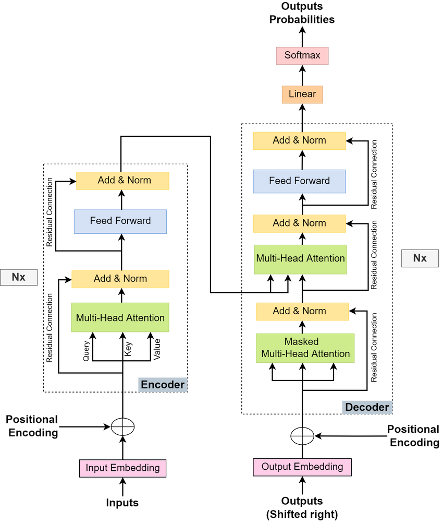
\includegraphics[width=0.75\textwidth]{images/transformer-architecture.png}
    \caption{Arsitektur dasar Transformer}
    \label{fig:transformer}
\end{figure}

Secara umum, proses kerja LLM dapat dijelaskan melalui beberapa tahapan berikut:

\begin{enumerate}
    \item \textit{Tokenization}: masukan teks diubah menjadi serangkaian token menggunakan metode seperti BPE (\textit{Byte Pair Encoding}) atau \textit{SentencePiece}. Token inilah yang diproses oleh model.

    \item \textit{Input Embedding}: setiap token direpresentasikan sebagai vektor berdimensi tinggi (misalnya 512--4096 dimensi), sehingga dapat diproses secara numerik oleh jaringan saraf.

    \item \textit{Positional Encoding}: karena Transformer tidak memiliki konsep urutan secara bawaan, informasi posisi ditambahkan menggunakan \textit{positional encoding} sinusoidal atau embedding terlatih lainnya.

    \item \textit{Multi-Head Self-Attention}: setiap token menghitung relevansinya terhadap token lain menggunakan tiga vektor utama: Query (Q), Key (K), dan Value (V). Mekanisme perhatian dihitung menggunakan rumus:

    \[
        \text{Attention}(Q, K, V) = \text{softmax}\left( \frac{QK^{T}}{\sqrt{d_k}} \right) V
    \]

    Mekanisme ini memungkinkan model mengidentifikasi konteks penting, dependensi jarak jauh, serta memahami relasi antar-token secara paralel melalui beberapa \textit{attention heads}.

    \item \textit{Feed-Forward Network (FFN)}: setiap token melewati jaringan \textit{feed-forward} dua lapis dengan aktivasi non-linear. Komponen ini memperluas kapasitas representasi sehingga model mampu melakukan transformasi dan \textit{reasoning} yang lebih kompleks.

    \item \textit{Output Softmax Layer}: pada tahap akhir, LLM memprediksi token berikutnya dengan memilih probabilitas tertinggi dari distribusi keluaran. Proses ini dilakukan secara autoregresif hingga seluruh respons terbentuk.
\end{enumerate}

Dengan kombinasi arsitektur Transformer dan pelatihan berskala besar, LLM memiliki kemampuan memahami konteks secara mendalam, menghasilkan teks yang koheren, serta menyesuaikan gaya bahasa sesuai kebutuhan pengguna.


\subsection{\textit{Prompt Engineering}}

\textit{Prompt} merupakan masukan teks yang diberikan pengguna untuk memandu model kecerdasan buatan, seperti LLM, dalam menghasilkan keluaran yang relevan dan sesuai tujuan. Dalam \textit{Prompt Engineering}, proses ini melibatkan perancangan \textit{prompt} yang efektif melalui pemilihan instruksi, konteks, contoh, serta batasan tertentu agar model dapat memberikan respons yang lebih akurat, terarah, dan konsisten. Teknik ini menjadi semakin penting karena performa LLM sangat bergantung pada cara instruksi dirumuskan dan seberapa jelas konteks yang diberikan \cite{Minaee2025PromptEngineering, White2023PromptPatternCatalog}.

Berbagai strategi \textit{prompt engineering} telah dikembangkan untuk meningkatkan performa LLM dalam menyelesaikan tugas-tugas kompleks. Beberapa teknik utama yang umum digunakan adalah sebagai berikut:

\begin{enumerate}
    \item \textit{Zero-Shot Prompting}: model diminta menyelesaikan tugas tanpa contoh sebelumnya, hanya berdasarkan instruksi.

    \item \textit{Few-Shot Prompting}: pengguna memberikan beberapa contoh masukan–keluaran untuk membimbing model menghasilkan respons yang serupa.

    \item \textit{Chain of Thought (CoT)}: instruksi meminta model menjelaskan proses berpikir secara bertahap, sehingga meningkatkan akurasi pada tugas penalaran.

    \item \textit{Tree of Thought (ToT)}: model mengeksplorasi beberapa jalur penalaran, mengevaluasi setiap opsi, kemudian memilih solusi terbaik.

    \item \textit{Self-Consistency}: model menghasilkan beberapa jalur penalaran yang kemudian digabungkan untuk memperoleh jawaban paling konsisten.

    \item \textit{Reflection Prompting}: setelah memberikan jawaban, model diminta melakukan evaluasi diri dan memperbaiki respons sebelumnya.

    \item \textit{Expert Prompting}: model diarahkan untuk bertindak sebagai seorang pakar dalam domain tertentu agar kualitas penjelasan lebih mendalam dan terstruktur.

    \item \textit{Rails / Guardrails}: pemberian batasan dan instruksi khusus agar model tetap fokus pada topik yang relevan serta mengurangi risiko \textit{hallucination}.

    \item \textit{Automatic Prompt Engineering (APE)}: menggunakan LLM untuk menghasilkan, menguji, dan memilih \textit{prompt} terbaik secara otomatis.
\end{enumerate}

Teknik-teknik tersebut digunakan untuk meningkatkan kontrol pengguna terhadap keluaran model, mengurangi risiko bias atau kesalahan, serta meningkatkan kualitas penjelasan dan kemampuan penalaran LLM dalam berbagai konteks pembelajaran maupun aplikasi praktis.

\subsection{Pemanfaatan LLM dalam Proses Pembelajaran}

Berbagai penelitian menunjukkan bahwa LLM semakin banyak dimanfaatkan sebagai sarana untuk memudahkan proses pembelajaran, baik sebagai tutor personal, penyedia umpan balik otomatis, maupun pendamping belajar mandiri. Kasneci dkk. \cite{Kasneci2023} mengidentifikasi bahwa LLM berpotensi meningkatkan personalisasi pembelajaran melalui kemampuannya menyesuaikan penjelasan dengan tingkat pemahaman pengguna, menyediakan umpan balik yang instan, serta mendukung akses belajar yang fleksibel tanpa batasan waktu dan tempat, sekaligus menyoroti tantangan terkait akurasi konten dan potensi ketergantungan berlebihan pada teknologi.

Dalam konteks pendidikan pemrograman, Leinonen dkk. \cite{Leinonen2023} menunjukkan bahwa LLM dapat digunakan untuk menerjemahkan pesan kesalahan pemrograman yang teknis menjadi penjelasan yang lebih mudah dipahami pemula, sehingga mempercepat proses \textit{debugging} dan mengurangi frustrasi belajar. Sejalan dengan itu, Jacobs dan Jaschke \cite{Jacobs2024LLMFeedbackProgramming} mengevaluasi penerapan LLM untuk menghasilkan umpan balik otomatis pada tugas pemrograman dan menemukan bahwa umpan balik yang dihasilkan cukup relevan serta membantu mahasiswa memahami letak kesalahan mereka secara mandiri.

Pemanfaatan LLM sebagai tutor personal juga dikaji oleh Vanzo dkk. \cite{Vanzo2024GPT4HomeworkTutor}, yang menemukan bahwa penggunaan GPT-4 sebagai pendamping mengerjakan tugas mampu meningkatkan keterlibatan dan capaian belajar mahasiswa dibandingkan metode belajar konvensional. Namun, tinjauan sistematis oleh Raihan dkk. \cite{Raihan2024} terhadap penerapan LLM dalam pendidikan ilmu komputer menegaskan bahwa manfaat tersebut hanya dapat dicapai secara konsisten apabila interaksi LLM diarahkan melalui mekanisme yang terstruktur, mengingat penggunaan LLM secara bebas berisiko menghasilkan penjelasan yang tidak konsisten atau menyimpang dari kurikulum.

Secara keseluruhan, pemanfaatan LLM dalam pembelajaran menunjukkan pergeseran peran teknologi dari sekadar alat pencarian informasi menjadi teman belajar interaktif yang mampu menjelaskan, mengoreksi, dan membimbing pengguna secara kontekstual. Temuan-temuan ini menjadi landasan bagi penelitian ini untuk mengembangkan Teman Belajar ASD sebagai aplikasi yang memanfaatkan LLM secara terarah guna mendukung proses belajar mandiri mahasiswa.

% Evaluasi
\section{Evaluasi}

Bagian ini membahas metode evaluasi yang digunakan untuk menilai kualitas dan kegunaan aplikasi yang dikembangkan. Kajian mencakup pendekatan \textit{black box testing} untuk verifikasi fungsionalitas sistem serta \textit{System Usability Scale} (SUS) sebagai instrumen pengukuran kegunaan.

\subsection{\textit{Black Box Testing}}

\textit{Black Box Testing} merupakan metode pengujian perangkat lunak yang berfokus pada evaluasi fungsi dan perilaku sistem dari sisi eksternal tanpa melihat struktur internal atau kode program. Pengujian dilakukan dengan memberikan berbagai \textit{input} dan memeriksa apakah \textit{output} yang dihasilkan telah sesuai dengan spesifikasi yang ditentukan \cite{Pressman2015SWE}.

Salah satu teknik \textit{Black Box Testing} yang banyak digunakan adalah \textit{Equivalence Partitioning}, yaitu pendekatan yang membagi domain \textit{input} ke dalam beberapa kelas ekivalen sehingga hanya satu nilai per kelas yang perlu diuji. Setiap nilai dalam kelas tersebut dianggap mewakili perilaku sistem untuk seluruh anggota kelas. Teknik ini membantu mengurangi jumlah \textit{test case} tanpa menurunkan efektivitas pengujian karena setiap partisi dirancang untuk menangkap potensi kesalahan berdasarkan kelompok \textit{input} yang memiliki karakteristik serupa \cite{Pressman2015SWE}.

Selain itu, pendekatan ini memperkuat efisiensi proses pengujian karena dapat meminimalkan redundansi dan meningkatkan cakupan pengujian. Konsep \textit{Equivalence Partitioning} juga didukung oleh pendekatan lain dalam pengujian perangkat lunak yang menekankan pentingnya representasi kelas nilai uji dalam mendeteksi kesalahan secara sistematis \cite{Myers2011ArtOfSoftwareTesting}. Dengan demikian, teknik ini menjadi salah satu metode yang efektif untuk memastikan bahwa fungsi utama perangkat lunak bekerja sesuai dengan spesifikasi yang telah ditetapkan.


\section{Penelitian Terdahulu}

Bagian ini mengulas penelitian-penelitian terdahulu yang relevan dengan topik pengembangan aplikasi pembelajaran ASD berbasis LLM. Kajian terhadap penelitian terdahulu dilakukan untuk mengidentifikasi pendekatan yang telah digunakan, hasil yang diperoleh, serta celah penelitian yang menjadi landasan pengembangan sistem dalam Tugas Akhir ini.

\subsection{\textit{Utilizing ChatGPT in a Data Structures and Algorithms Course: A Teaching Assistant's Perspective}}

Pemanfaatan ChatGPT sebagai alat bantu \textit{Teaching Assistant} (TA) dalam mata kuliah \textit{Data Structures and Algorithms} (DSA) terbukti efektif dalam meningkatkan kualitas pembelajaran. Studi oleh Jamie et al. \cite{Jamie2024ChatGPTDSA} menunjukkan bahwa penggunaan LLM seperti ChatGPT-4o dan ChatGPT-o1 dapat membantu mahasiswa memahami konsep algoritmik kompleks melalui penjelasan terstruktur, pembuatan contoh, dan penyediaan latihan berbasis \textit{structured prompts}. Dalam pendekatan ini, keluaran LLM tetap diverifikasi oleh TA untuk menjaga akurasi dan kesesuaian konten.

Hasil eksperimen terkontrol membandingkan dua kelas---kelas dengan instruksi tradisional dan kelas dengan pendekatan hibrida TA dengan ChatGPT. Kelompok hibrida menunjukkan peningkatan signifikan dengan selisih rata-rata 16{,}50 poin lebih tinggi pada latihan, kuis, dan ujian. Model AI membantu menjelaskan konsep sulit seperti rekursi, \textit{graph traversal}, serta \textit{dynamic programming}, sembari menyajikan keluaran yang lebih terarah berkat \textit{prompt} yang sistematis.

Namun, penelitian tersebut juga mencatat keterbatasan ChatGPT, seperti ketidakmampuan menghasilkan visualisasi struktur data dan potensi kesalahan pada masalah yang memerlukan kreativitas tinggi. Dengan demikian, peran TA tetap penting untuk memvalidasi keluaran model. Studi ini menegaskan bahwa integrasi LLM tidak menggantikan peran manusia, melainkan memperkuat efektivitas pengajaran melalui kolaborasi manusia dan AI yang terstruktur.


\subsection{\textit{Evaluating the Effectiveness of Large Language Models in Solving Simple Programming Tasks: A User-Centered Study}}

Penelitian oleh Deng \cite{Deng2025LLMProgrammingTasks} mengevaluasi efektivitas tiga gaya interaksi ChatGPT-4o, \textit{Passive}, \textit{Proactive}, dan \textit{Collaborative}, dalam membantu pengguna menyelesaikan tugas pemrograman sederhana. Pada mode \textit{Passive}, model hanya merespons permintaan. Pada mode \textit{Proactive}, model memberikan saran tambahan, sedangkan mode \textit{Collaborative} memungkinkan diskusi dua arah yang lebih intens.

Sebanyak lima belas siswa sekolah menengah diminta menyelesaikan tiga soal pemrograman di setiap mode interaksi. Hasil eksperimen menunjukkan bahwa mode \textit{Collaborative} menghasilkan waktu penyelesaian tercepat, yaitu rata-rata 2{,}63 menit per soal, dibandingkan mode \textit{Passive} yang membutuhkan rata-rata 3{,}60 menit. Hal ini menunjukkan bahwa kualitas interaksi berperan penting dalam efektivitas penggunaan LLM.

Selain peningkatan performa, peserta juga melaporkan tingkat kepuasan dan persepsi kebermanfaatan yang lebih tinggi pada mode \textit{Collaborative}. Temuan ini menegaskan bahwa interaksi yang bersifat dialogis membantu pengguna memahami langkah penyelesaian masalah dengan lebih baik.


\subsection{\textit{Leveraging Algorithm Instruction with AI Chatbots: A Detailed Exploration of Their Impact on Students' Computational Thinking}}

Penggunaan \textit{AI-based chatbots} sebagai pendukung pembelajaran algoritma turut dievaluasi oleh Zaus et al. \cite{Zaus2025AlgorithmInstructionChatbots}. Melalui pendekatan \textit{quasi-experimental}, penelitian ini membandingkan kelompok mahasiswa yang belajar dengan bantuan \textit{chatbot} dan kelompok yang menggunakan metode pembelajaran konvensional.

Hasil \textit{pre-test} dan \textit{post-test} menunjukkan peningkatan signifikan pada pemahaman konsep algoritma dan keterampilan \textit{computational thinking} dalam kelompok yang menggunakan \textit{chatbot}. Hal ini terjadi karena \textit{chatbot} menyediakan penjelasan langkah demi langkah, umpan balik otomatis, serta dukungan koreksi kesalahan yang membuat proses belajar lebih interaktif dan mudah diikuti.

Penelitian ini juga menemukan bahwa \textit{chatbot} dapat berfungsi sebagai bentuk \textit{scaffolding}, membantu mahasiswa mengatasi miskonsepsi pada materi yang kompleks, serta menyesuaikan tingkat kesulitan penyampaian materi berdasarkan respons pengguna. Dengan demikian, pengalaman belajar menjadi lebih personal dan adaptif.


% ============================================================================================
% BAB III ANALISIS MASALAH
% Pembagian subbab tidak rigid dan dapat bervariasi. Bab ini minimal berisi analisis kebutuhan
% fungsional, analisis berbagai alternatif solusi yang dapat ditawarkan, dan
% metode pemilihan solusi yang diusulkan.
% ============================================================================================
\cleardoublepage
\chapter{ANALISIS MASALAH}
\label{chap:analisis-masalah}

Bab ini membahas analisis permasalahan yang mendasari pengembangan sistem pembelajaran Algoritma dan Struktur Data (ASD) berbasis \textit{Large Language Model} (LLM) dengan pendekatan \textit{guided learning}. Secara garis besar, bab ini membahas hal-hal berikut:

\begin{enumerate}[1.]
    \item Analisis kondisi pembelajaran ASD saat ini, meliputi fungsi umum sistem yang sudah ada beserta permasalahan yang masih ditemui;
    \item Analisis kebutuhan sistem, mencakup identifikasi masalah pengguna, konsep dasar solusi yang diusulkan, serta rumusan kebutuhan fungsional; dan
    \item Analisis pemilihan solusi, meliputi evaluasi berbagai alternatif teknologi dan penentuan solusi yang paling sesuai untuk mendukung pengembangan sistem.
\end{enumerate}


% ============================================================
\section{Analisis Kondisi Saat Ini}
% ============================================================

Pembelajaran Algoritma dan Struktur Data (ASD) merupakan salah satu komponen penting dalam kurikulum ilmu komputer yang bertujuan membekali mahasiswa dengan kemampuan memahami struktur data, merancang algoritma, serta menganalisis kompleksitas program. Meskipun demikian, berbagai studi menunjukkan bahwa proses pembelajaran ASD masih menghadapi tantangan signifikan, terutama dalam penyampaian konsep yang bersifat abstrak dan dinamis \autocite{Mtaho2024}. Berdasarkan studi literatur dan observasi terhadap praktik pembelajaran saat ini, bagian berikut merangkum fungsi-fungsi utama sistem pembelajaran ASD yang digunakan mahasiswa serta berbagai kendala yang masih ditemui dalam implementasinya.

Adapun fungsi umum yang dimiliki sistem pembelajaran ASD saat ini, yaitu:

\begin{enumerate}
    \item Menyediakan materi pembelajaran dalam bentuk modul, \textit{slide}, dan contoh kode yang dapat digunakan mahasiswa untuk mempelajari konsep dasar, seperti \textit{array}, \textit{linked list}, \textit{stack}, \textit{queue}, \textit{tree}, \textit{graph}, serta algoritma \textit{searching} dan \textit{sorting}.
    \item Menyediakan penjelasan dan ilustrasi visual melalui diagram atau animasi sederhana untuk membantu mahasiswa memahami perubahan struktur data secara bertahap.
    \item Memberikan latihan soal dan kuis yang berfungsi menguji pemahaman mahasiswa terhadap konsep algoritmik tertentu.
    \item Menyediakan forum diskusi atau sesi tanya jawab dengan dosen dan asisten pengajar untuk membantu menjelaskan konsep yang membingungkan atau memperbaiki miskonsepsi.
    \item Menggunakan \textit{environment} pemrograman seperti IDE atau \textit{notebook} untuk memungkinkan mahasiswa mencoba implementasi kode secara langsung.
\end{enumerate}

Meskipun telah menyediakan fitur-fitur tersebut, pendekatan pembelajaran ASD saat ini masih memiliki berbagai permasalahan, antara lain:

\begin{enumerate}
    \item Sistem pembelajaran umumnya bersifat statis dan tidak adaptif terhadap kebutuhan mahasiswa. Materi, contoh, dan penjelasan yang tersedia biasanya disajikan dalam satu format yang sama sehingga tidak dapat menyesuaikan tingkat pemahaman setiap mahasiswa. Kondisi ini membuat mahasiswa yang mengalami kesulitan pada konsep tertentu tidak mendapatkan penjelasan tambahan yang lebih terarah.

    \item Penjelasan mengenai struktur data yang bersifat dinamis, seperti \textit{linked list}, \textit{tree}, atau \textit{graph}, sering kali masih kurang intuitif karena hanya ditampilkan dalam bentuk gambar statis. Hal ini menyulitkan mahasiswa untuk memahami perubahan \textit{pointer}, hubungan antar-\textit{node}, atau proses algoritma secara rinci.

    \item Mahasiswa sering mengandalkan penjelasan dari asisten pengajar atau sumber eksternal seperti \textit{chatbot} LLM umum. Namun, penggunaan LLM secara bebas memiliki keterbatasan, seperti ketidakkonsistenan dengan kurikulum atau potensi terjadinya \textit{hallucination} yang dapat menghasilkan informasi keliru.

    \item Umpan balik terhadap latihan dan pemahaman konsep biasanya tidak diberikan secara cepat. Mahasiswa harus menunggu sesi asistensi atau waktu koreksi, sehingga proses belajar menjadi kurang responsif dan memperlambat perbaikan miskonsepsi.

    \item Sumber referensi materi sering kali tersebar pada berbagai platform seperti LMS, modul digital, forum diskusi, dan sumber eksternal lain, sehingga tidak ada satu wadah terintegrasi yang dapat memandu mahasiswa mengikuti alur belajar secara sistematis.
\end{enumerate}

Saat ini, proses pembelajaran ASD di lingkungan perkuliahan masih sangat bergantung pada metode tradisional yang membutuhkan interaksi langsung dengan dosen atau asisten pengajar. Meskipun LLM modern seperti ChatGPT, Gemini, atau DeepSeek mulai dimanfaatkan oleh mahasiswa, penggunaannya belum terintegrasi dengan kurikulum dan tidak dibatasi oleh struktur pembelajaran tertentu. Kondisi ini membuat mahasiswa berisiko menerima penjelasan yang tidak sesuai urutan materi atau bahkan bertentangan dengan pendekatan yang diajarkan dalam kelas.


% ============================================================
\section{Analisis Kebutuhan}
% ============================================================

Bagian ini menguraikan analisis kebutuhan sistem pembelajaran ASD berbasis \textit{guided learning}. Analisis dimulai dari identifikasi permasalahan yang dihadapi pengguna dalam proses pembelajaran ASD saat ini, kemudian dilanjutkan dengan penggambaran konsep dasar sistem yang diusulkan sebagai solusi, dan diakhiri dengan penjabaran kebutuhan fungsional yang harus dipenuhi oleh sistem.

\subsection{Identifikasi Masalah Pengguna}

Pengguna utama sistem ini adalah mahasiswa yang mempelajari materi Algoritma dan Struktur Data (ASD). Dalam proses pembelajaran saat ini, mahasiswa sering menghadapi berbagai tantangan karena materi ASD memiliki tingkat abstraksi yang tinggi, bersifat dinamis, dan memerlukan kemampuan penalaran algoritmik yang kuat \autocite{Mtaho2024}. Metode pembelajaran tradisional yang mengandalkan modul, \textit{slide}, serta penjelasan langsung dari dosen dan asisten pengajar belum sepenuhnya mampu menjawab kebutuhan mahasiswa dalam memahami konsep secara mendalam dan bertahap. Kondisi ini menyebabkan mahasiswa sering mengalami miskonsepsi pada konsep dasar, kesulitan mengikuti alur materi, serta kurangnya umpan balik cepat ketika mengalami kebingungan.

Selain itu, mahasiswa kerap mencari bantuan melalui \textit{chatbot} LLM umum, namun interaksi yang tidak terarah dan tidak sesuai materi yang diberikan di kelas berpotensi memberikan penjelasan keliru atau tidak konsisten \autocite{White2023PromptPatternCatalog}. Hal ini memperlambat proses belajar dan meningkatkan risiko kesalahan pemahaman. Berikut permasalahan yang dihadapi oleh pengguna tersebut.

\begin{enumerate}
    \item Mahasiswa saat ini belum memiliki sistem pembelajaran yang menyajikan penjelasan konsep ASD secara terstruktur dan bertahap sehingga memudahkan mereka membangun pemahaman dari dasar hingga tingkat yang lebih kompleks.

    \item Mahasiswa tidak memiliki akses terhadap contoh implementasi kode dan ilustrasi langkah demi langkah yang dapat disesuaikan dengan tingkat pemahaman mereka.

    \item Mahasiswa belum memiliki sistem pembelajaran yang mampu memberikan penjelasan, contoh, dan latihan yang konsisten dengan materi karena penggunaan LLM umum tidak dibatasi oleh kurikulum atau konteks materi resmi.

    \item Mahasiswa tidak mendapatkan peringatan atau umpan balik otomatis ketika terjadi miskonsepsi dalam memahami konsep, seperti kesalahan logika pada struktur data atau salah menafsirkan alur algoritma.

    \item Mahasiswa belum memiliki sistem terpadu yang dapat memberikan ringkasan materi yang relevan berdasarkan konteks materi yang sedang mereka pelajari.

    \item Mahasiswa tidak mendapatkan dukungan untuk mengecek pemahaman mereka secara langsung karena latihan dan evaluasi sering kali tidak memberikan penjelasan balik atau pembahasan detail.

    \item Mahasiswa belum memiliki sistem yang mendukung analisis lebih mendalam melalui visualisasi perubahan struktur data dan simulasi algoritma dalam berbagai skenario untuk memperkuat pemahaman konseptual mereka.

    \item Mahasiswa tidak memiliki sarana untuk mengujikan soal dari sumber eksternal (buku, soal ujian terdahulu, atau latihan mandiri) dan mendapatkan evaluasi otomatis terhadap jawaban mereka dalam konteks materi ASD.

    \item Mahasiswa tidak memiliki akses terhadap asisten tanya-jawab yang mampu menjawab pertanyaan kontekstual secara langsung sesuai topik yang sedang dipelajari tanpa harus menunggu sesi asistensi.
\end{enumerate}

Untuk mencari solusi atas masalah-masalah tersebut, perlu disusun kebutuhan fungsional sistem yang diperlukan. Berikut penjabaran mengenai kebutuhan fungsional untuk sistem yang akan dibuat.


\subsection{Konsep Dasar Sistem yang Diusulkan}

Konsep dasar sistem pembelajaran yang diusulkan pada tugas akhir ini berfokus pada pemanfaatan \textit{Large Language Model} (LLM) dalam kerangka \textit{guided learning} yang terstruktur untuk membantu mahasiswa memahami materi Algoritma dan Struktur Data (ASD) secara lebih efektif. Sistem ini dirancang untuk mengatasi berbagai permasalahan pembelajaran yang telah diidentifikasi pada bagian sebelumnya, khususnya terkait sifat materi yang abstrak, perlunya penjelasan bertahap, keterbatasan sumber belajar statis, serta ketidakkonsistenan penjelasan ketika menggunakan \textit{chatbot} umum.

Secara konsep, sistem ini berfungsi sebagai pendamping belajar yang memberikan alur pembelajaran terarah meliputi penjelasan konsep, contoh implementasi, latihan soal, dan ringkasan materi. Setiap tahap pembelajaran dihasilkan oleh LLM namun tetap dikendalikan melalui struktur \textit{prompt} dan konteks materi kuliah yang disediakan oleh dosen. Dengan demikian, sistem tidak hanya menghasilkan penjelasan secara generatif, tetapi melakukannya dengan batasan dan struktur yang selaras dengan kurikulum resmi \autocite{Minaee2025PromptEngineering}.

Selain menyediakan konten terarah, sistem ini juga dirancang untuk memberikan umpan balik otomatis terhadap jawaban mahasiswa pada latihan soal. Dengan adanya umpan balik instan, mahasiswa dapat mengetahui letak kesalahan mereka secara cepat sehingga proses koreksi miskonsepsi dapat berlangsung lebih efektif tanpa harus menunggu sesi asistensi atau evaluasi manual dari pengajar.

Secara keseluruhan, konsep dasar sistem ini adalah menghadirkan platform pembelajaran ASD yang:

\begin{enumerate}
    \item terstruktur melalui tahapan \textit{guided learning} yang konsisten,
    \item adaptif dengan kemampuan LLM menghasilkan penjelasan sesuai konteks materi dan kebutuhan pengguna,
    \item responsif dengan pemberian umpan balik otomatis untuk mendukung koreksi pemahaman, dan
    \item terpadu sebagai satu wadah pembelajaran yang menggabungkan materi, contoh, latihan, dan ringkasan secara sistematis.
\end{enumerate}


\subsection{Kebutuhan Fungsional}

Kebutuhan fungsional atau \textit{Functional Requirements} merupakan kebutuhan-kebutuhan dalam bentuk layanan yang diberikan oleh sistem kepada pengguna. Berikut merupakan tabel kebutuhan fungsional dari sistem pembelajaran Algoritma dan Struktur Data berbasis \textit{Large Language Model} dengan pendekatan \textit{guided learning}.

\begin{longtable}{|L{1.8cm}|L{3cm}|L{7.5cm}|}
\caption{Kebutuhan Fungsional Sistem Pembelajaran ASD Berbasis LLM}
\label{tab:kebutuhan-fungsional}\\
\hline
\textbf{ID} & \textbf{Kebutuhan} & \textbf{Penjelasan} \\
\hline
\endfirsthead

\caption[]{Kebutuhan Fungsional Sistem Pembelajaran ASD Berbasis LLM (lanjutan)}\\
\hline
\textbf{ID} & \textbf{Kebutuhan} & \textbf{Penjelasan} \\
\hline
\endhead

\hline
\multicolumn{3}{l}{\textit{Bersambung ke halaman berikutnya}}\\
\endfoot

\hline
\endlastfoot

FR-01 & Sistem mampu menampilkan alur pembelajaran ASD yang terstruktur &
Sistem dirancang untuk menampilkan alur belajar yang terdiri dari tahapan penjelasan konsep, contoh implementasi, latihan soal, dan ringkasan. Pengguna dapat memilih topik materi, lalu sistem menampilkan urutan langkah yang harus diikuti agar pembelajaran menjadi lebih terarah. \\
\hline

FR-02 & Sistem mampu menghasilkan penjelasan konsep ASD berbasis LLM sesuai konteks materi &
Sistem memanfaatkan LLM dengan struktur \textit{prompt} yang terarah untuk menghasilkan penjelasan konsep yang relevan, akurat, serta konsisten dengan materi yang sedang dipelajari pengguna. \\
\hline

FR-03 & Sistem mampu menampilkan contoh kode dan penjelasan langkah demi langkah &
Sistem dapat menghasilkan contoh implementasi kode untuk topik tertentu, disertai penjelasan langkah demi langkah mengenai alur eksekusi algoritma dan perubahan struktur data. Fitur ini membantu pengguna memahami hubungan antara konsep teoretis dan implementasi program. \\
\hline

FR-04 & Sistem mampu menyediakan latihan soal dan pembahasan otomatis &
Sistem dapat menghasilkan atau menampilkan latihan soal yang terkait dengan materi yang sedang dipelajari pengguna. Setelah pengguna menjawab, sistem memberikan pembahasan otomatis yang menjelaskan alasan jawaban benar maupun salah. \\
\hline

FR-05 & Sistem mampu memberikan umpan balik terhadap miskonsepsi pengguna &
Sistem menganalisis jawaban atau interaksi pengguna untuk mengidentifikasi pola kesalahan umum, kemudian memberikan umpan balik yang menjelaskan letak miskonsepsi serta mengarahkan pengguna kembali ke penjelasan yang sesuai. \\
\hline

FR-06 & Sistem mampu menyajikan ringkasan materi pada akhir sesi belajar &
Sistem dapat menghasilkan ringkasan materi yang telah dipelajari pada suatu sesi, termasuk poin penting, istilah kunci, dan hubungan antar konsep. Ringkasan ini membantu pengguna melakukan \textit{review} dan memperkuat pemahaman konsep. \\
\hline

FR-07 & Sistem mampu menyimpan dan menampilkan riwayat serta progres belajar pengguna &
Sistem menyimpan data riwayat topik yang sudah dipelajari, latihan yang telah dikerjakan, serta status penyelesaian tiap modul. Pengguna dapat melihat progres belajarnya dan melanjutkan pembelajaran dari posisi terakhir dengan mudah. \\
\hline

FR-08 & Sistem mampu menerima dan mengevaluasi soal yang diunggah pengguna &
Sistem menyediakan fasilitas bagi pengguna untuk memasukkan soal dari sumber eksternal beserta jawabannya secara mandiri. Sistem kemudian mengevaluasi jawaban menggunakan LLM berdasarkan konteks materi topik yang sedang dipelajari dan mengembalikan hasil evaluasi berupa skor, komentar, bagian yang sudah benar, bagian yang perlu diperbaiki, serta rekomendasi belajar. \\
\hline

FR-09 & Sistem mampu memberikan penjelasan materi melalui asisten percakapan kontekstual berbasis LLM &
Sistem menyediakan asisten percakapan (\textit{chat asisten materi}) yang memungkinkan pengguna mengajukan pertanyaan seputar materi topik yang sedang dipelajari. Asisten menggunakan konteks materi resmi sebagai landasan jawaban sehingga penjelasan yang dihasilkan tetap relevan dan konsisten dengan kurikulum ASD. Riwayat percakapan dipertahankan selama sesi berlangsung untuk mendukung tanya-jawab yang berkesinambungan. \\
\hline

\end{longtable}

Dengan memenuhi kebutuhan fungsional ini, sistem diharapkan dapat memberikan solusi yang membantu pengguna dalam mengatasi berbagai permasalahan pembelajaran ASD yang telah diidentifikasi sebelumnya.




% ============================================================
\section{Analisis Pemilihan Solusi}
% ============================================================

Bagian ini memaparkan analisis pemilihan teknologi dan pendekatan yang digunakan dalam pengembangan sistem pembelajaran ASD. Analisis mencakup tinjauan terhadap berbagai alternatif solusi yang tersedia, mencakup perbandingan model LLM dan pendekatan pembelajaran, serta justifikasi pemilihan solusi akhir yang paling sesuai dengan kebutuhan sistem.

\subsection{Alternatif Solusi}

Penentuan alternatif solusi dilakukan dengan mempertimbangkan setiap kebutuhan dari permasalahan pembelajaran ASD, khususnya kebutuhan penjelasan yang terarah, konsistensi dengan materi kuliah, serta kemampuan menghasilkan contoh dan latihan secara otomatis. Bagian berikut menguraikan alternatif teknologi yang dapat digunakan dalam pengembangan sistem pembelajaran ASD berbasis LLM, serta pertimbangan pemilihan solusi yang paling sesuai.

\subsubsection{Pemilihan Model LLM}

Terdapat beberapa pilihan model LLM yang populer dalam pengembangan aplikasi edukasi berbasis AI, di antaranya GPT-4o, Gemini 1.5, dan Claude 3. Masing-masing model memiliki kelebihan dan kekurangan dalam hal kemampuan \textit{reasoning}, kualitas penjelasan teknis, serta konsistensi keluaran.

GPT-4o unggul dalam pemahaman konteks yang panjang, penalaran algoritmik, dan kemampuan memberikan penjelasan langkah demi langkah secara stabil, sebagaimana ditunjukkan oleh performanya yang konsisten di atas model-model pendahulunya pada berbagai \textit{benchmark} penalaran dan pemrograman seperti MMLU dan HumanEval \autocite{OpenAI2023GPT4TechnicalReport}. Model ini terbukti efektif untuk menghasilkan contoh kode, menyusun latihan, serta memberikan umpan balik yang terstruktur, menjadikannya kandidat kuat untuk sistem pembelajaran yang memerlukan penjelasan mendalam dalam domain pemrograman \autocite{Jacobs2024LLMFeedbackProgramming}. Selain itu, studi lain menunjukkan bahwa GPT-4 yang berperan sebagai tutor tugas mampu meningkatkan keterlibatan (\textit{engagement}) dan capaian belajar mahasiswa dibandingkan metode belajar konvensional \autocite{Vanzo2024GPT4HomeworkTutor}. Namun, GPT-4o memerlukan biaya penggunaan yang relatif lebih tinggi dibandingkan beberapa alternatif lainnya.

Di sisi lain, Gemini 1.5 menawarkan kapasitas konteks yang sangat besar sehingga cocok untuk sistem yang memerlukan penyertaan modul kuliah atau dokumen panjang dalam \textit{prompt}. Akan tetapi, kualitas \textit{reasoning} Gemini pada permasalahan algoritmik tertentu kadang kurang stabil dan lebih mudah menghasilkan jawaban yang tidak konsisten.

Claude 3 memiliki kemampuan penjelasan natural dan terstruktur, tetapi terkadang kurang presisi dalam contoh kode yang kompleks, khususnya pada topik algoritma tingkat lanjut.

Perbandingan ketiga model LLM tersebut dirangkum pada Tabel~\ref{tab:perbandingan-llm}.

\begin{longtable}{|L{2.9cm}|L{3.3cm}|L{3.3cm}|L{2.4cm}|}
\caption{Perbandingan Model LLM untuk Sistem Pembelajaran ASD}
\label{tab:perbandingan-llm}\\
\hline
\textbf{Kriteria} & \textbf{GPT-4o} & \textbf{Gemini 1.5} & \textbf{Claude 3} \\
\hline
\endfirsthead

\caption[]{Perbandingan Model LLM untuk Sistem Pembelajaran ASD (lanjutan)}\\
\hline
\textbf{Kriteria} & \textbf{GPT-4o} & \textbf{Gemini 1.5} & \textbf{Claude 3} \\
\hline
\endhead

\hline
\multicolumn{4}{l}{\textit{Bersambung ke halaman berikutnya}}\\
\endfoot

\hline
\endlastfoot

\textit{Reasoning} algoritmik & Sangat baik, stabil & Cukup baik, kurang konsisten & Baik, terkadang kurang presisi \\
\hline
Kualitas penjelasan teknis & Mendalam dan sistematis & Cukup baik & Natural, kurang detail pada kode kompleks \\
\hline
Konsistensi keluaran & Tinggi & Sedang & Tinggi \\
\hline
Kapasitas konteks & Besar & Sangat besar & Besar \\
\hline
Biaya penggunaan & Relatif tinggi & Menengah & Menengah \\
\hline
Kesesuaian untuk ASD & Sangat sesuai & Cukup sesuai & Cukup sesuai \\
\hline

\end{longtable}


\subsection{Analisis Penentuan Solusi}

Berdasarkan hasil evaluasi terhadap berbagai alternatif solusi yang telah diuraikan pada subbab sebelumnya, berikut adalah keputusan pemilihan solusi yang digunakan dalam pengembangan sistem pembelajaran ASD berbasis LLM.

\subsubsection{Model LLM yang Dipilih}

Setelah mempertimbangkan seluruh aspek yang relevan, GPT-4o dipilih sebagai model LLM utama yang digunakan dalam sistem ini. Pemilihan GPT-4o didasarkan pada beberapa pertimbangan berikut:

\begin{enumerate}
    \item \textbf{Kemampuan \textit{reasoning} yang tinggi dan stabil.} GPT-4o menunjukkan konsistensi yang baik dalam menghasilkan penjelasan algoritmik yang akurat, terutama untuk topik-topik yang memerlukan penalaran bertahap seperti proses traversal pada \textit{tree} atau analisis kompleksitas algoritma, sejalan dengan hasil pengujian \textit{benchmark} yang menunjukkan keunggulan model ini pada tugas penalaran dan pemrograman \autocite{OpenAI2023GPT4TechnicalReport}.

    \item \textbf{Kualitas contoh kode dan umpan balik yang baik.} Model ini mampu menghasilkan contoh implementasi kode dalam berbagai bahasa pemrograman dengan kualitas yang memadai, disertai penjelasan langkah demi langkah yang mudah dipahami. Efektivitas model keluarga GPT-4 dalam menghasilkan umpan balik pemrograman yang relevan bagi mahasiswa juga telah dikonfirmasi pada penelitian sebelumnya \autocite{Jacobs2024LLMFeedbackProgramming}, sekaligus mendukung perannya sebagai teman belajar digital yang terbukti dapat meningkatkan keterlibatan dan capaian belajar mahasiswa \autocite{Vanzo2024GPT4HomeworkTutor}.

    \item \textbf{Dukungan terhadap \textit{prompt engineering} yang terstruktur.} GPT-4o merespons dengan baik terhadap instruksi dan batasan yang diberikan melalui \textit{system prompt}, sehingga memungkinkan sistem untuk mengendalikan format keluaran sesuai tahapan \textit{guided learning} \autocite{White2023PromptPatternCatalog}.

    \item \textbf{Ekosistem API yang matang.} OpenAI menyediakan API yang stabil dan terdokumentasi dengan baik, mempermudah integrasi dengan \textit{backend} aplikasi.
\end{enumerate}

Dengan pertimbangan tersebut, GPT-4o memberikan keseimbangan terbaik antara kemampuan teknis, stabilitas keluaran, dan kemudahan integrasi untuk mendukung sistem pembelajaran ASD yang terarah, akurat, dan konsisten dengan kurikulum.

\subsubsection{Pendekatan \textit{Guided Learning}}

Selain pemilihan model LLM, pendekatan pembelajaran yang digunakan dalam sistem ini juga merupakan bagian krusial dari solusi yang diusulkan. Pendekatan \textit{guided learning} dipilih karena kemampuannya dalam menyediakan alur belajar yang terstruktur dan terarah, berbeda dengan pendekatan \textit{open-ended chat} yang tidak memiliki batasan konteks. Dengan pendekatan ini, setiap sesi pembelajaran mahasiswa akan mengikuti urutan tahapan yang konsisten, yaitu:

\begin{enumerate}
    \item \textbf{Penjelasan Konsep}: LLM menghasilkan penjelasan teoretis yang disesuaikan dengan topik yang dipilih mahasiswa, mencakup definisi, karakteristik, dan hubungan dengan konsep lain dalam ASD.

    \item \textbf{Contoh Implementasi}: LLM menyajikan contoh kode beserta penjelasan alur eksekusi secara langkah demi langkah, membantu mahasiswa menghubungkan teori dengan praktik pemrograman.

    \item \textbf{Latihan Soal}: Sistem menyediakan soal latihan yang relevan dengan materi, disertai pembahasan otomatis setelah mahasiswa menjawab untuk mendeteksi dan mengoreksi miskonsepsi secara langsung.

    \item \textbf{Ringkasan}: LLM menghasilkan ringkasan poin-poin penting dari sesi belajar yang telah selesai sebagai bahan \textit{review} bagi mahasiswa.
\end{enumerate}

Pendekatan ini memastikan bahwa seluruh konten yang dihasilkan LLM tetap relevan, terstruktur, dan konsisten dengan kurikulum resmi, sekaligus memberikan pengalaman belajar yang lebih terarah dan efektif dibandingkan interaksi bebas dengan \textit{chatbot} umum.


% ==========================================
% BAB IV PERANCANGAN
% ==========================================
\cleardoublepage
\chapter{PERANCANGAN}
\label{chap:perancangan}

\section{Gambaran Umum Sistem}

\subsection{Use Case}

Pada sistem aplikasi pembelajaran Algoritma dan Struktur Data berbasis \textit{guided learning} ini, terdapat satu aktor yaitu \textit{user} yang merupakan mahasiswa sebagai pengguna sistem. \textit{User} berinteraksi dengan sistem untuk mempelajari materi ASD secara terstruktur, mulai dari memilih topik, memahami konsep, melihat contoh, mengerjakan latihan, hingga memantau progres belajar.

Sistem dirancang sebagai \textit{teman belajar digital} yang mendampingi mahasiswa dalam proses pembelajaran. Melalui integrasi LLM, sistem mampu memberikan penjelasan materi, contoh implementasi, serta umpan balik terhadap latihan yang dikerjakan oleh \textit{user} secara interaktif dan adaptif.

Berikut merupakan \textit{use case diagram} yang menggambarkan interaksi antara \textit{user} dengan sistem pembelajaran ASD.

\begin{figure}[H]
    \centering
    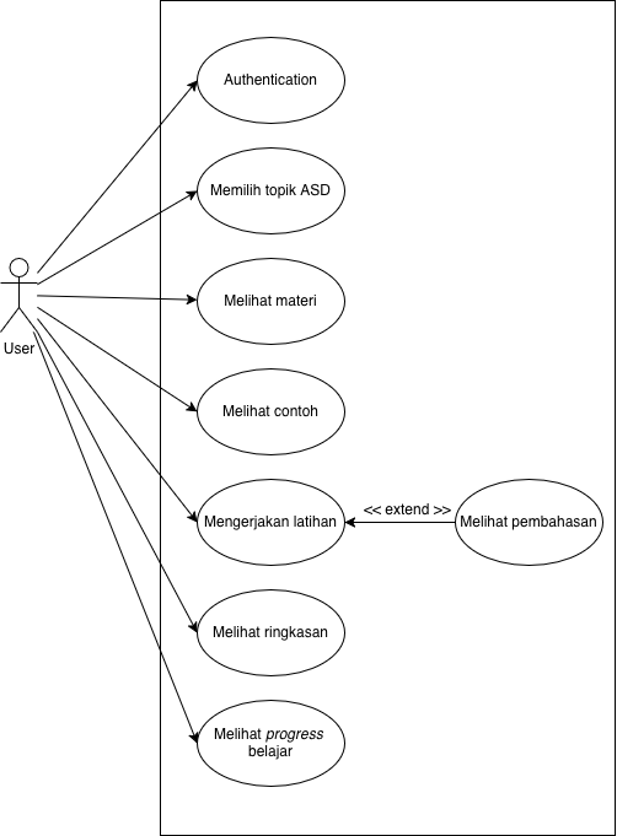
\includegraphics[width=0.75\textwidth]{images/use-case-diagram.png}
    \caption{Diagram \textit{Use Case} Sistem Teman Belajar ASD}
    \label{fig:use-case}
\end{figure}

Penjelasan mengenai diagram di atas dan keterkaitannya dengan kebutuhan fungsional dapat dilihat pada Tabel \ref{tab:use-case}.

\begin{longtable}{|p{1.2cm}|p{1.5cm}|p{2.8cm}|p{5.5cm}|p{1.8cm}|}
\caption{Deskripsi \textit{Use Case} Sistem Pembelajaran ASD}
\label{tab:use-case}\\
\hline
\textbf{ID} & \textbf{Aktor} & \textbf{Use Case} & \textbf{Deskripsi} & \textbf{Functional Requirements} \\
\hline
\endfirsthead

\caption[]{Deskripsi \textit{Use Case} Sistem Pembelajaran ASD (lanjutan)}\\
\hline
\textbf{ID} & \textbf{Aktor} & \textbf{Use Case} & \textbf{Deskripsi} & \textbf{Functional Requirements} \\
\hline
\endhead

\hline
\multicolumn{5}{r}{\textit{Bersambung ke halaman berikutnya}}\\
\endfoot

\hline
\endlastfoot

UC-01 & User & Authentication &
User melakukan \textit{login} dengan memasukkan kredensial berupa \textit{email} dan \textit{password} untuk mengakses sistem pembelajaran. &
FR-01 \\
\hline

UC-02 & User & Memilih topik ASD &
User memilih topik pembelajaran ASD yang ingin dipelajari sebagai langkah awal dalam alur belajar. &
FR-02 \\
\hline

UC-03 & User & Melihat materi &
User menerima penjelasan konsep ASD yang dihasilkan sistem secara terstruktur sesuai topik yang dipilih. &
FR-03 \\
\hline

UC-04 & User & Melihat contoh &
User melihat contoh implementasi atau ilustrasi dari konsep ASD untuk membantu pemahaman. &
FR-04 \\
\hline

UC-05 & User & Mengerjakan latihan &
User mengerjakan soal latihan yang diberikan sistem untuk menguji pemahaman terhadap materi. &
FR-05 \\
\hline

UC-06 & User & Melihat pembahasan &
User melihat pembahasan dari latihan yang telah dikerjakan sebagai bentuk umpan balik dari sistem. Relasi \textit{extend} dari UC-05 menunjukkan bahwa pembahasan hanya tersedia setelah \textit{user} mengerjakan latihan. &
FR-06 \\
\hline

UC-07 & User & Melihat ringkasan &
User melihat rangkuman materi untuk memperkuat pemahaman terhadap konsep yang telah dipelajari. &
FR-07 \\
\hline

UC-08 & User & Melihat \textit{progress} belajar &
User dapat melihat progres pembelajaran yang menunjukkan sejauh mana materi telah dipelajari. &
FR-08 \\
\hline

\end{longtable}

Tabel \ref{tab:use-case} menunjukkan bahwa terdapat satu aktor yaitu \textit{user} yang dapat menjalankan berbagai aktivitas untuk memenuhi kebutuhan fungsional sistem. Proses pembelajaran dimulai dari \textit{user} melakukan autentikasi (UC-01), kemudian memilih topik ASD yang ingin dipelajari (UC-02).

Selanjutnya, \textit{user} akan memasuki alur pembelajaran terstruktur dengan melihat materi (UC-03) yang berisi penjelasan konsep yang dihasilkan sistem. Untuk memperdalam pemahaman, \textit{user} dapat melihat contoh implementasi (UC-04) sebelum mengerjakan latihan yang diberikan (UC-05).

Setelah menyelesaikan latihan, \textit{user} dapat melihat pembahasan (UC-06) sebagai bentuk umpan balik dari sistem. Relasi \textit{extend} antara UC-05 dan UC-06 menunjukkan bahwa pembahasan hanya muncul setelah \textit{user} mengerjakan latihan. Selain itu, \textit{user} juga dapat melihat ringkasan materi (UC-07) untuk memperkuat pemahaman, serta memantau progres belajar melalui fitur \textit{progress} (UC-08).

Dengan demikian, seluruh \textit{use case} yang dirancang telah mencerminkan alur \textit{guided learning} yang mendukung pembelajaran ASD secara terstruktur dan interaktif, serta memenuhi kebutuhan fungsional sistem.


\subsection{Sequence Diagram}

\textit{Sequence diagram} menggambarkan urutan interaksi antar komponen sistem, \textit{User}, \textit{Frontend}, \textit{Backend}, \textit{Database}, dan OpenAI API, dalam menyelesaikan setiap fungsionalitas. Diagram berikut disusun berdasarkan alur \textit{guided learning} yang telah dirancang, mulai dari autentikasi hingga pemantauan progres belajar.

\begin{figure}[H]
    \centering
    \textbf{FT-01 Login}\\[6pt]
    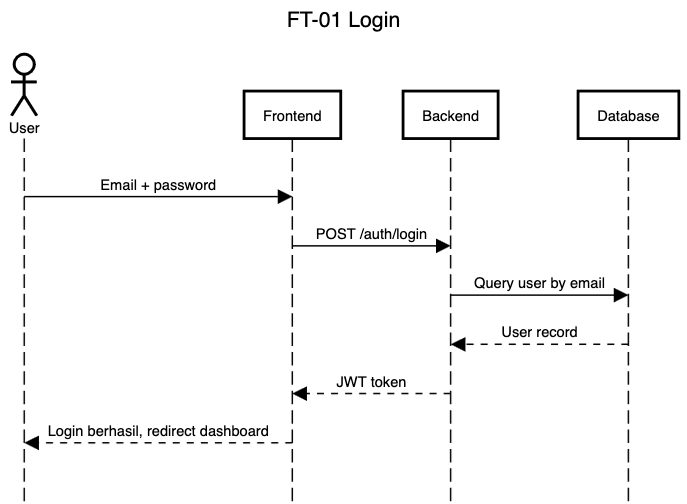
\includegraphics[width=0.9\textwidth]{images/FT-01-Login.png}
    \caption{\textit{Sequence Diagram} FT-01 Login}
    \label{fig:sd-login}
\end{figure}

Diagram pada Gambar \ref{fig:sd-login} menggambarkan alur autentikasi pengguna. \textit{User} memasukkan \textit{email} dan \textit{password} pada \textit{frontend}, yang kemudian mengirimkan permintaan \texttt{POST /auth/login} ke \textit{backend}. \textit{Backend} melakukan \textit{query} data pengguna ke \textit{database} berdasarkan \textit{email} yang diberikan. Jika data ditemukan dan kredensial valid, \textit{backend} mengembalikan JWT \textit{token} ke \textit{frontend}, yang selanjutnya menyimpan \textit{token} tersebut dan mengarahkan \textit{user} ke halaman \textit{dashboard}.

\begin{figure}[H]
    \centering
    \textbf{FT-02 Logout}\\[6pt]
    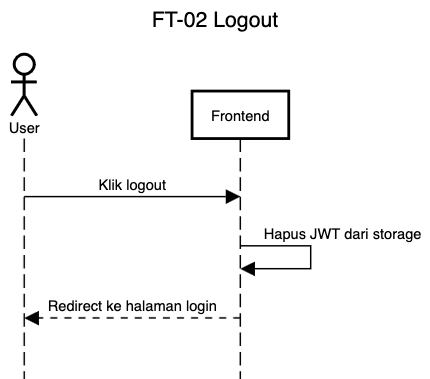
\includegraphics[width=0.55\textwidth]{images/FT-02-Logout.png}
    \caption{\textit{Sequence Diagram} FT-02 Logout}
    \label{fig:sd-logout}
\end{figure}

Diagram pada Gambar \ref{fig:sd-logout} menggambarkan alur keluar dari sistem. Ketika \textit{user} mengeklik tombol \textit{logout}, \textit{frontend} langsung menghapus JWT \textit{token} dari \textit{storage} lokal tanpa perlu melakukan panggilan ke \textit{backend}. Setelah \textit{token} dihapus, \textit{frontend} mengarahkan \textit{user} kembali ke halaman \textit{login}.

\begin{figure}[H]
    \centering
    \textbf{FT-03 Pilih Topik ASD + FT-11 \textit{Guided Learning Flow}}\\[6pt]
    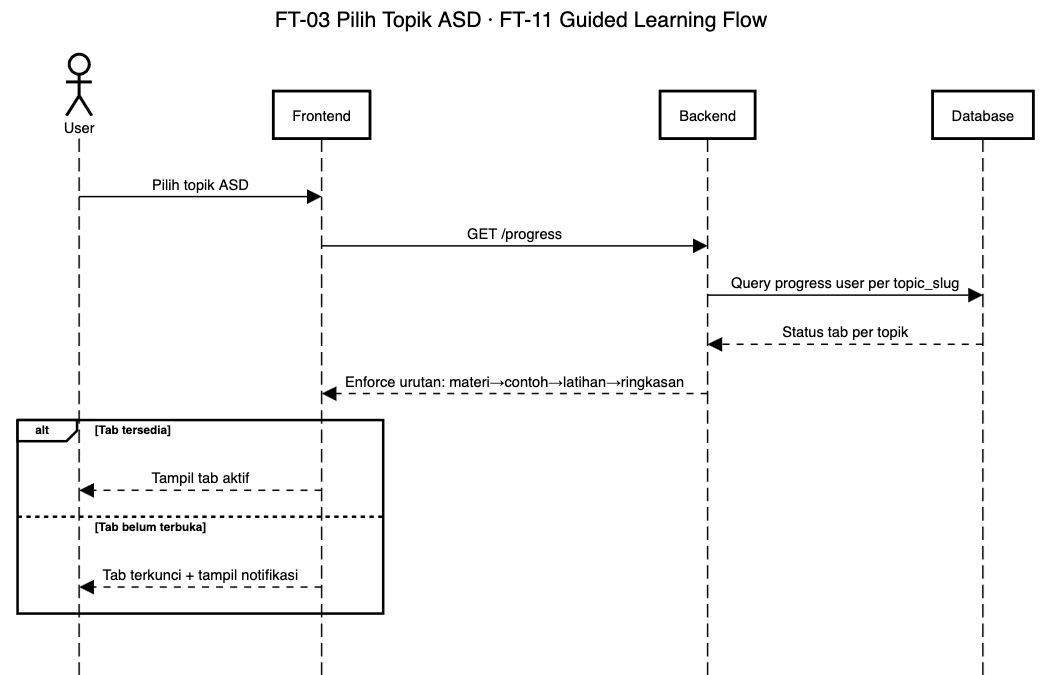
\includegraphics[width=0.9\textwidth]{images/FT-03-Pilih-Topik-ASD-FT-11-Guided-Learning-Flow.png}
    \caption{\textit{Sequence Diagram} FT-03 Pilih Topik ASD dan FT-11 \textit{Guided Learning Flow}}
    \label{fig:sd-pilih-topik}
\end{figure}

Diagram pada Gambar \ref{fig:sd-pilih-topik} menggambarkan alur pemilihan topik ASD sekaligus penegakan urutan \textit{guided learning}. Setelah \textit{user} memilih topik, \textit{frontend} meminta data progres melalui \texttt{GET /progress}. \textit{Backend} mengambil status tab tiap topik dari \textit{database}, lalu menegakkan urutan pembelajaran: materi $\rightarrow$ contoh $\rightarrow$ latihan $\rightarrow$ ringkasan. Jika tab yang ingin diakses sudah tersedia, sistem menampilkan tab tersebut; jika belum terbuka, sistem menguncinya dan menampilkan notifikasi kepada \textit{user}.

\begin{figure}[H]
    \centering
    \textbf{FT-04 Tampilkan Materi + FT-10 \textit{Generate} LLM + FT-14 Adaptasi Konten}\\[6pt]
    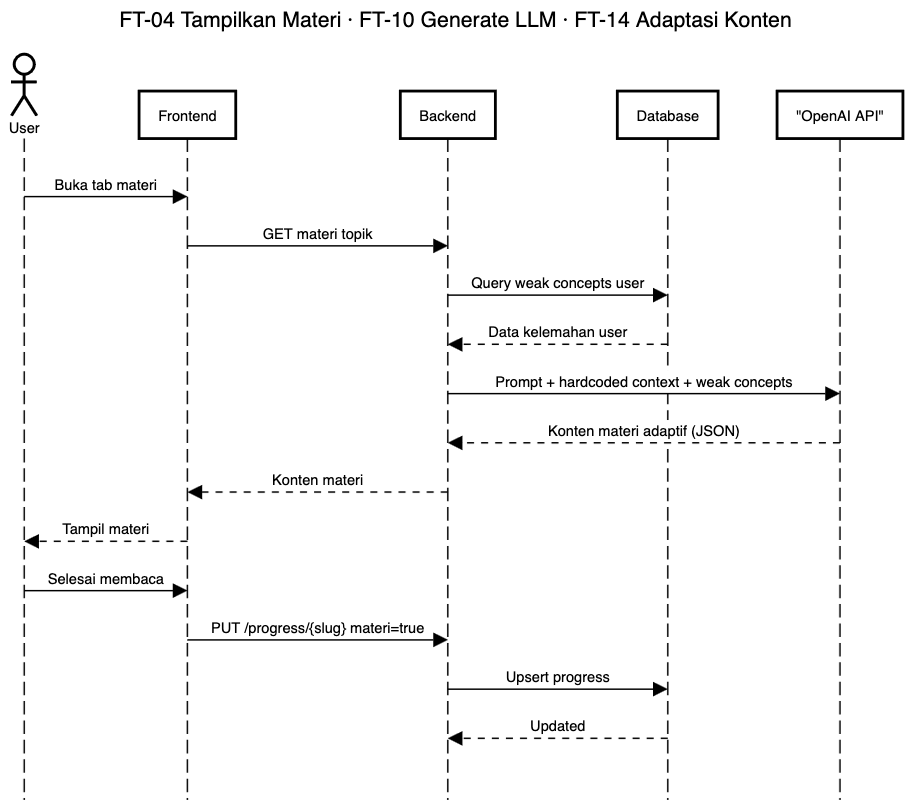
\includegraphics[width=0.9\textwidth]{images/FT-04-Tampilkan-Materi-FT-10-Generate-LLM-FT-14-Adaptasi-Konten.png}
    \caption{\textit{Sequence Diagram} FT-04 Tampilkan Materi, FT-10 \textit{Generate} LLM, dan FT-14 Adaptasi Konten}
    \label{fig:sd-materi}
\end{figure}

Diagram pada Gambar \ref{fig:sd-materi} menggambarkan alur penampilan materi yang dihasilkan LLM secara adaptif. Ketika \textit{user} membuka tab materi, \textit{frontend} mengirim permintaan ke \textit{backend}. \textit{Backend} terlebih dahulu mengambil data kelemahan konsep \textit{user} (\textit{weak concepts}) dari \textit{database}, kemudian menyusun \textit{prompt} yang menggabungkan konteks materi (\textit{hardcoded context}) dan data kelemahan tersebut sebelum dikirim ke OpenAI API. Respons berupa konten materi adaptif dalam format JSON dikembalikan ke \textit{frontend} dan ditampilkan kepada \textit{user}. Setelah \textit{user} selesai membaca, \textit{frontend} memperbarui progres melalui \texttt{PUT /progress/\{slug\}} dengan status \texttt{materi=true}.

\begin{figure}[H]
    \centering
    \textbf{FT-05 Tampilkan Contoh + FT-10 \textit{Generate} LLM + FT-14 Adaptasi Konten}\\[6pt]
    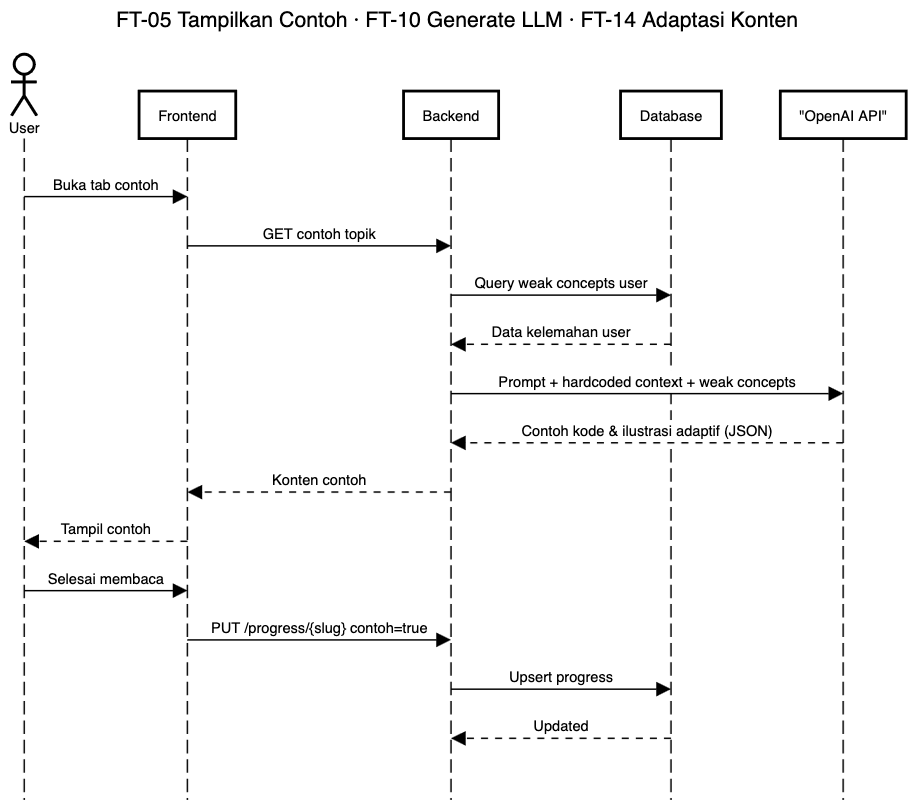
\includegraphics[width=0.9\textwidth]{images/FT-05-Tampilkan-Contoh-FT-10-Generate-LLM-FT-14-Adaptasi-Konten.png}
    \caption{\textit{Sequence Diagram} FT-05 Tampilkan Contoh, FT-10 \textit{Generate} LLM, dan FT-14 Adaptasi Konten}
    \label{fig:sd-contoh}
\end{figure}

Diagram pada Gambar \ref{fig:sd-contoh} menggambarkan alur penampilan contoh implementasi yang bersifat adaptif. Alur ini serupa dengan FT-04, namun keluaran yang dihasilkan OpenAI API berupa contoh kode dan ilustrasi langkah demi langkah yang disesuaikan dengan kelemahan konsep \textit{user}. Setelah \textit{user} selesai mempelajari contoh, progres diperbarui dengan status \texttt{contoh=true} sehingga tab latihan dapat dibuka.

\begin{figure}[H]
    \centering
    \textbf{FT-06 Latihan Soal + FT-10 \textit{Generate} LLM + FT-13 \textit{Adaptive Engine} + FT-14 Adaptasi Konten}\\[6pt]
    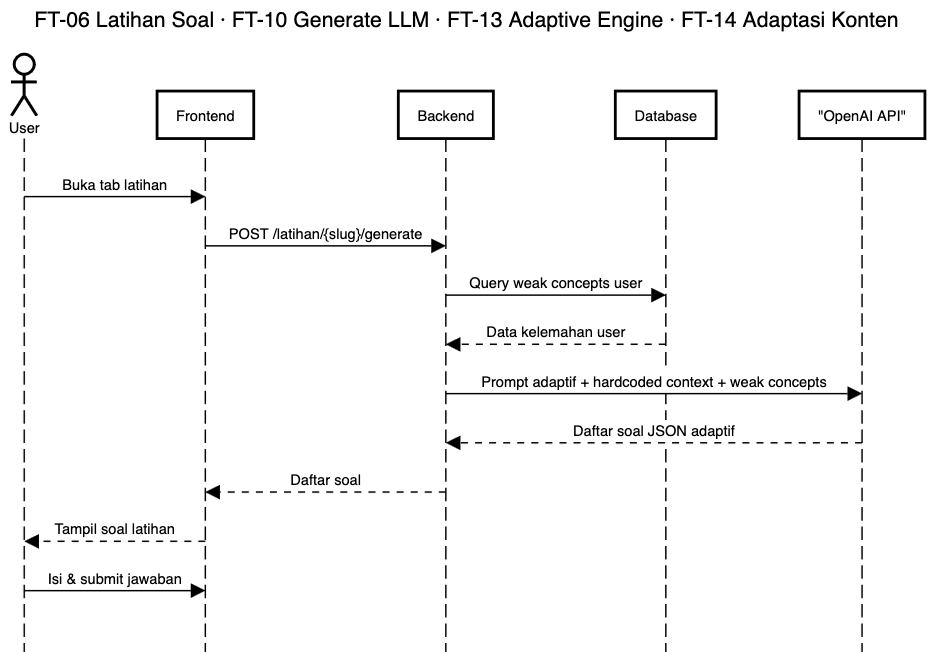
\includegraphics[width=0.9\textwidth]{images/FT-06-Latihan-Soal-FT-10-Generate-LLM-FT-13-Adaptive-Engine-FT-14-Adaptasi-Konten.png}
    \caption{\textit{Sequence Diagram} FT-06 Latihan Soal, FT-10 \textit{Generate} LLM, FT-13 \textit{Adaptive Engine}, dan FT-14 Adaptasi Konten}
    \label{fig:sd-latihan}
\end{figure}

Diagram pada Gambar \ref{fig:sd-latihan} menggambarkan alur pembuatan dan penyajian latihan soal secara adaptif. \textit{Frontend} mengirim permintaan \texttt{POST /latihan/\{slug\}/generate} ke \textit{backend}. \textit{Backend} mengambil data \textit{weak concepts} dari \textit{database} dan menyusun \textit{prompt} adaptif yang memprioritaskan konsep-konsep yang masih lemah bagi \textit{user}. OpenAI API menghasilkan daftar soal dalam format JSON yang kemudian ditampilkan kepada \textit{user}. \textit{User} mengisi jawaban dan melakukan \textit{submit} untuk dievaluasi pada tahap berikutnya.

\begin{figure}[H]
    \centering
    \textbf{FT-07 Pembahasan Latihan + FT-12 \textit{Feedback} Jawaban + FT-13 \textit{Adaptive Engine}}\\[6pt]
    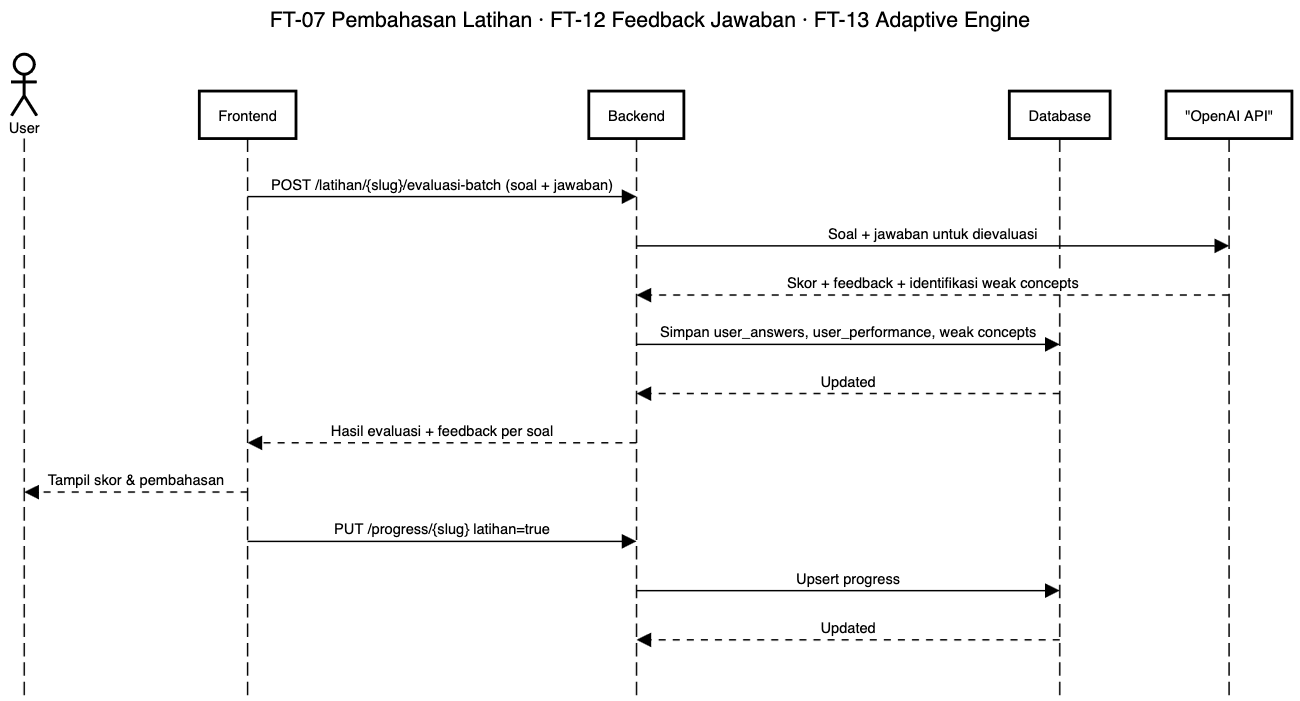
\includegraphics[width=0.9\textwidth]{images/FT-07-Pembahasan-Latihan-FT-12-Feedback-Jawaban-FT-13-Adaptive-Engine.png}
    \caption{\textit{Sequence Diagram} FT-07 Pembahasan Latihan, FT-12 \textit{Feedback} Jawaban, dan FT-13 \textit{Adaptive Engine}}
    \label{fig:sd-pembahasan}
\end{figure}

Diagram pada Gambar \ref{fig:sd-pembahasan} menggambarkan alur evaluasi jawaban dan pembaruan model adaptif. Setelah \textit{user} mengirim jawaban, \textit{frontend} meneruskan seluruh pasangan soal dan jawaban ke \textit{backend} melalui \texttt{POST /latihan/\{slug\}/evaluasi-batch}. \textit{Backend} mengirimkan data tersebut ke OpenAI API untuk dievaluasi, dan API mengembalikan skor, \textit{feedback} per soal, serta identifikasi \textit{weak concepts} baru. \textit{Backend} menyimpan hasil evaluasi — termasuk \texttt{user\_answers}, \texttt{user\_performance}, dan \textit{weak concepts} — ke \textit{database} untuk digunakan sebagai dasar adaptasi pada sesi berikutnya. \textit{Frontend} kemudian menampilkan skor dan pembahasan kepada \textit{user}, dan memperbarui progres dengan status \texttt{latihan=true}.

\begin{figure}[H]
    \centering
    \textbf{FT-08 Ringkasan Materi}\\[6pt]
    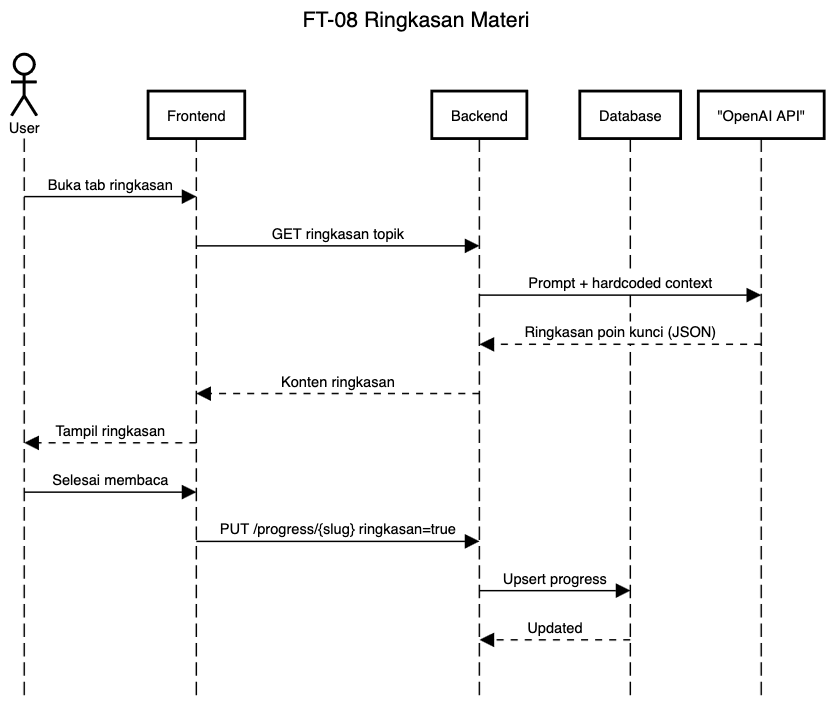
\includegraphics[width=0.9\textwidth]{images/FT-08-Ringkasan-Materi.png}
    \caption{\textit{Sequence Diagram} FT-08 Ringkasan Materi}
    \label{fig:sd-ringkasan}
\end{figure}

Diagram pada Gambar \ref{fig:sd-ringkasan} menggambarkan alur penampilan ringkasan materi di akhir sesi belajar. \textit{Frontend} mengirim permintaan \texttt{GET} ringkasan ke \textit{backend}, yang kemudian meneruskan \textit{prompt} beserta konteks materi ke OpenAI API. API menghasilkan ringkasan poin-poin kunci dalam format JSON. Setelah \textit{user} selesai membaca ringkasan, progres diperbarui dengan status \texttt{ringkasan=true}, menandakan bahwa \textit{user} telah menyelesaikan seluruh tahapan pembelajaran untuk topik tersebut.

\begin{figure}[H]
    \centering
    \textbf{FT-09 Progres Belajar + FT-13 \textit{Adaptive Engine}}\\[6pt]
    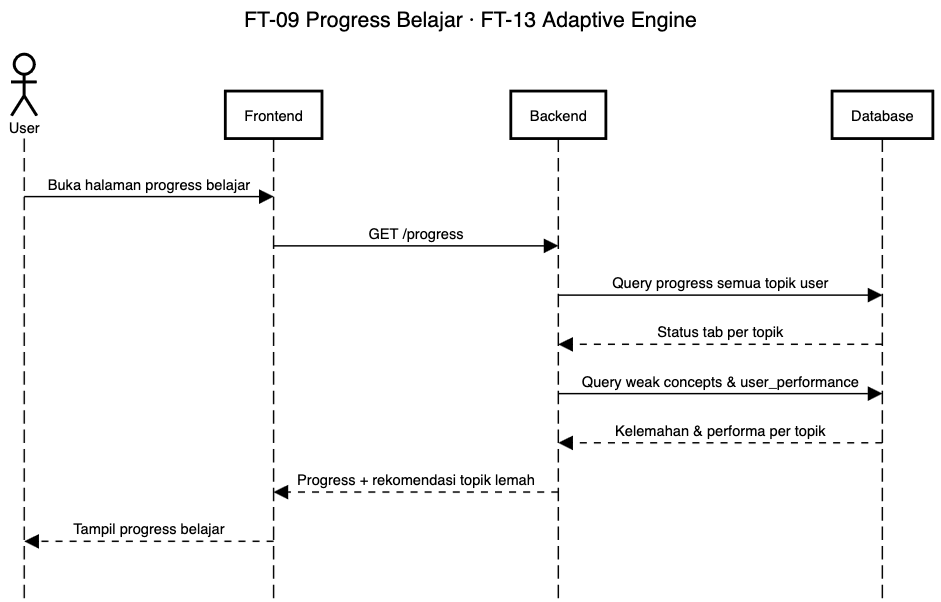
\includegraphics[width=0.9\textwidth]{images/FT-09-Progress-Belajar-FT-13-Adaptive-Engine.png}
    \caption{\textit{Sequence Diagram} FT-09 Progres Belajar dan FT-13 \textit{Adaptive Engine}}
    \label{fig:sd-progress}
\end{figure}

Diagram pada Gambar \ref{fig:sd-progress} menggambarkan alur penampilan halaman progres belajar yang terintegrasi dengan \textit{adaptive engine}. \textit{Frontend} meminta data melalui \texttt{GET /progress}, dan \textit{backend} melakukan dua \textit{query} ke \textit{database}: pertama untuk mengambil status tab seluruh topik, dan kedua untuk mengambil data \textit{weak concepts} serta performa \textit{user} per topik. \textit{Backend} menggabungkan kedua data tersebut dan mengembalikan informasi progres lengkap beserta rekomendasi topik yang perlu diperkuat. \textit{Frontend} menampilkan seluruh informasi tersebut kepada \textit{user} dalam satu halaman yang komprehensif.


\section{Perancangan \textit{Database}}

\subsection{Spesifikasi \textit{Platform Database}}

PostgreSQL dipilih sebagai sistem manajemen \textit{database} karena bersifat \textit{open source}, mendukung tipe data relasional yang kaya, serta memiliki ekosistem yang matang untuk pengembangan aplikasi web. Akses ke \textit{database} dilakukan melalui SQLAlchemy sebagai ORM (\textit{Object-Relational Mapper}) dengan \textit{driver} psycopg3, sehingga interaksi antara \textit{backend} Python dan \textit{database} dapat dilakukan secara efisien dan aman. Tabel \ref{tab:spek-db} menyajikan spesifikasi \textit{platform database} yang digunakan.

\begin{table}[H]
    \centering
    \caption{Spesifikasi \textit{Platform Database}}
    \label{tab:spek-db}
    \begin{tabular}{|p{4cm}|p{8cm}|}
    \hline
    \textbf{Aspek} & \textbf{Spesifikasi} \\
    \hline
    \textit{Database Engine} & PostgreSQL \\
    \hline
    \textit{Driver} & psycopg (psycopg3) \\
    \hline
    ORM & SQLAlchemy \\
    \hline
    Nama \textit{Database} & \texttt{asd\_learning\_db} \\
    \hline
    Port & 5432 (default) \\
    \hline
    \end{tabular}
\end{table}

\subsection{Desain Skema \textit{Database}}
\section{Perancangan \textit{Website}}
\subsection{Perancangan API}
\subsection{Perancangan Antarmuka}
Will be attached later
\subsection{Spesifikasi \textit{Hosting}}

% ==========================================
% BAB V IMPLEMENTASI
% ==========================================
\cleardoublepage
\chapter{IMPLEMENTASI WEBSITE PEMBELAJARAN ALGORITMA DAN STRUKTUR DATA BERBASIS \textit{GUIDED LEARNING}}
\label{chap:implementasi}

Bab ini membahas proses implementasi sistem Teman Belajar ASD berdasarkan hasil perancangan yang telah diuraikan pada Bab IV. Implementasi dilakukan secara bertahap, dimulai dari penyiapan lingkungan pengembangan, pembangunan komponen \textit{frontend} dengan Next.js, hingga pengembangan \textit{backend} berbasis FastAPI beserta integrasi OpenAI API sebagai mesin generasi konten adaptif. Seluruh hasil implementasi mengacu pada kebutuhan fungsional dan nonfungsional yang telah ditetapkan.

\section{Lingkungan Implementasi}

Pada pengembangan sistem Teman Belajar ASD dibutuhkan perangkat baik sisi perangkat keras maupun perangkat lunak untuk mendukung proses implementasi. Penjelasan lingkungan implementasi pada sisi perangkat keras yang digunakan dapat dilihat pada Tabel \ref{tab:impl-hardware}.

\begin{table}[H]
    \centering
    \caption{Lingkungan Implementasi Perangkat Keras}
    \label{tab:impl-hardware}
    \begin{tabular}{|p{4.5cm}|p{8cm}|}
    \hline
    \textbf{Spesifikasi} & \textbf{Detail} \\
    \hline
    Perangkat & Laptop MacBook Pro \\
    \hline
    Prosesor & Apple Silicon M1 \\
    \hline
    RAM & 16 GB \\
    \hline
    Penyimpanan Internal & SSD 512 GB \\
    \hline
    \end{tabular}
\end{table}

Selain lingkungan perangkat keras, implementasi sistem ini membutuhkan dukungan perangkat lunak yang terpasang pada perangkat keras. Penjelasan lingkungan implementasi pada sisi perangkat lunak yang digunakan dapat dilihat pada Tabel \ref{tab:impl-software}.

\begin{table}[H]
    \centering
    \caption{Lingkungan Implementasi Perangkat Lunak}
    \label{tab:impl-software}
    \begin{tabular}{|p{4.5cm}|p{8cm}|}
    \hline
    \textbf{Spesifikasi} & \textbf{Detail} \\
    \hline
    Sistem Operasi & macOS Sequoia 15 \\
    \hline
    \textit{Text Editor} & Visual Studio Code \\
    \hline
    Bahasa Pemrograman & Python 3.11, JavaScript (Node.js 20) \\
    \hline
    \textit{Frontend Framework} & Next.js 16, React 19, Tailwind CSS 4 \\
    \hline
    \textit{Backend Framework} & FastAPI, SQLAlchemy, Pydantic \\
    \hline
    \textit{Containerization} & Docker \\
    \hline
    \textit{Repository} & GitHub \\
    \hline
    \textit{Cloud Platform} & Google Cloud Platform (Cloud Run, Artifact Registry) \\
    \hline
    CI/CD & GitHub Actions \\
    \hline
    \end{tabular}
\end{table}

Dengan terpenuhinya kebutuhan lingkungan implementasi yang sesuai, implementasi sistem Teman Belajar ASD diharapkan dapat berjalan dengan lancar.

\section{Implementasi \textit{Frontend}}

\section{Implementasi \textit{Backend}}

% ==========================================
% BAB VI EVALUASI
% ==========================================
\cleardoublepage
\chapter{EVALUASI}
\label{chap:evaluasi}

\section{Metode Evaluasi}

Evaluasi Aplikasi Pembelajaran ASD dilakukan untuk memastikan bahwa sistem yang dikembangkan telah memenuhi seluruh kebutuhan fungsional yang ditetapkan, menghasilkan konten pembelajaran yang berkualitas, serta dapat digunakan dengan mudah oleh mahasiswa sebagai pengguna. Evaluasi terdiri atas dua bagian utama, yaitu pengujian \textit{black box} untuk memverifikasi fungsionalitas sistem dan pengujian kegunaan (\textit{usability testing}) untuk menilai pengalaman pengguna secara keseluruhan.

\subsection{Pengujian \textit{Black Box}}

\textit{Black Box Testing} merupakan metode pengujian perangkat lunak yang mengevaluasi fungsi dan perilaku sistem dari sisi eksternal tanpa melihat struktur internal atau kode program, sehingga pengujian dilakukan dengan memberikan berbagai \textit{input} dan memeriksa apakah \textit{output} telah sesuai dengan spesifikasi yang ditentukan \cite{Pressman2015SWE}. Pada pengujian ini digunakan teknik \textit{Equivalence Partitioning}, yaitu metode yang membagi domain \textit{input} ke dalam beberapa kelas ekivalen sehingga hanya satu nilai dari setiap kelas yang perlu diuji karena dianggap mewakili seluruh anggota kelas tersebut \cite{Myers2011ArtOfSoftwareTesting}.

Pengujian \textit{black box} dilakukan terhadap seluruh fitur fungsional Aplikasi Pembelajaran ASD berdasarkan kebutuhan fungsional yang telah ditetapkan. Setiap fitur diuji dengan mendefinisikan skenario uji, data masukan, keluaran yang diharapkan, dan status kelulusan. Rangkuman cakupan pengujian \textit{black box} dapat dilihat pada Tabel \ref{tab:blackbox} berikut.

\begin{longtable}{|L{0.9cm}|L{2.3cm}|L{4.4cm}|L{4.4cm}|}
\caption{Cakupan Pengujian \textit{Black Box}}
\label{tab:blackbox}\\
\hline
\textbf{ID} & \textbf{Fitur} & \textbf{Skenario Uji} & \textbf{Indikator Keberhasilan} \\
\hline
\endfirsthead

\caption[]{Cakupan Pengujian \textit{Black Box} (lanjutan)}\\
\hline
\textbf{ID} & \textbf{Fitur} & \textbf{Skenario Uji} & \textbf{Indikator Keberhasilan} \\
\hline
\endhead

\hline
\multicolumn{4}{r}{\textit{Bersambung ke halaman berikutnya}}\\
\endfoot

\hline
\endlastfoot

FT-01 & Pilih Topik ASD &
Pengguna memilih salah satu dari sepuluh topik yang tersedia &
Sistem menampilkan halaman topik dengan tab sesuai status \textit{guided flow} pengguna \\
\hline

FT-02 & Tampilkan Materi &
Pengguna membuka tab materi pada topik yang dipilih &
Konten materi statis berhasil dirender dan ditampilkan sesuai topik, progres diperbarui setelah selesai dibaca \\
\hline

FT-03 & Tampilkan Contoh &
Pengguna membuka tab contoh setelah menyelesaikan tab materi &
Konten contoh berhasil dihasilkan dan ditampilkan, tab terkunci jika materi belum selesai \\
\hline

FT-04 & Latihan Soal &
Pengguna membuka tab latihan dan menerima soal yang di-\textit{generate} &
Soal latihan berhasil di-\textit{generate} oleh LLM dan ditampilkan kepada pengguna \\
\hline

FT-05 & Pembahasan Latihan &
Pengguna mengumpulkan jawaban latihan &
Sistem mengembalikan skor, \textit{feedback} per soal, dan pembahasan yang relevan \\
\hline

FT-06 & Ringkasan Materi &
Pengguna membuka tab ringkasan setelah menyelesaikan latihan &
Konten ringkasan statis berhasil dirender dan ditampilkan, topik ditandai selesai \\
\hline

FT-07 & Progres Belajar &
Pengguna membuka halaman progres belajar &
Sistem menampilkan status penyelesaian seluruh topik beserta indikator kelemahan konsep \\
\hline

FT-08 & \textit{Generate} Konten LLM &
Sistem mengirim \textit{prompt} ke OpenAI API untuk menghasilkan materi, contoh, dan soal &
OpenAI API mengembalikan konten dalam format JSON yang valid sesuai topik \\
\hline

FT-09 & \textit{Guided Learning Flow} &
Pengguna mencoba mengakses tab yang belum terbuka &
Sistem mengunci tab yang belum tersedia dan menampilkan notifikasi untuk menyelesaikan tahap sebelumnya \\
\hline

FT-10 & \textit{Feedback} Jawaban &
Pengguna mengumpulkan jawaban latihan &
Sistem menampilkan \textit{feedback} spesifik per soal beserta skor yang akurat \\
\hline

FT-11 & \textit{Adaptive Learning Engine} &
Pengguna menyelesaikan latihan dengan hasil tertentu &
Sistem menyimpan \textit{weak concepts} dan menggunakannya pada \textit{generate} soal berikutnya \\
\hline

FT-12 & Adaptasi Konten Pembelajaran &
Pengguna dengan riwayat \textit{weak concepts} membuka materi/contoh/latihan &
Konten yang dihasilkan lebih menekankan konsep yang teridentifikasi sebagai kelemahan pengguna \\
\hline

FT-13 & Evaluasi Soal Sendiri &
Pengguna memasukkan soal dan jawaban dari sumber eksternal pada panel Soal Sendiri. Skenario uji meliputi soal berisi teks, soal diunggah dari file \texttt{.txt}, dan kolom jawaban dikosongkan &
Sistem mengembalikan hasil evaluasi berisi skor, nilai, komentar, bagian benar/salah, dan rekomendasi belajar. Soal tanpa jawaban mendapat nilai "Belum Dijawab" \\
\hline

FT-14 & Chat Asisten Materi &
Pengguna mengirim pertanyaan melalui \textit{widget chat} pada halaman topik aktif, skenario uji meliputi pertanyaan relevan dengan topik dan pertanyaan lanjutan yang mengacu pada jawaban sebelumnya &
Sistem mengembalikan balasan kontekstual yang relevan dengan materi topik, pertanyaan lanjutan dijawab dengan mempertimbangkan riwayat percakapan \\
\hline

\end{longtable}


\subsection{Pengujian Kegunaan (\textit{Usability Testing})}

Selain pengujian fungsional, dilakukan pengujian kegunaan untuk menilai sejauh mana aplikasi dapat digunakan oleh mahasiswa dengan mudah, efisien, dan memuaskan. Pengujian kegunaan dilakukan melalui dua pendekatan, yaitu \textit{task-based usability test} dan pengisian kuesioner \textit{System Usability Scale} (SUS).

\subsubsection{\textit{Task-Based Usability Test}}

\textit{Task-based usability test} dilakukan dengan meminta responden menyelesaikan serangkaian tugas yang mencerminkan alur penggunaan aplikasi secara nyata. Responden diminta untuk menyelesaikan tugas-tugas berikut secara berurutan tanpa bantuan dari peneliti:

\begin{enumerate}
    \item Memilih salah satu topik ASD dari halaman \textit{dashboard}.
    \item Membaca konten materi dan menandai tab materi sebagai selesai.
    \item Membuka tab contoh dan membaca contoh implementasi yang ditampilkan.
    \item Mengerjakan latihan soal dan mengumpulkan seluruh jawaban.
    \item Membaca pembahasan dan skor yang diberikan sistem.
    \item Membuka tab ringkasan dan menyelesaikan alur belajar satu topik.
    \item Mengakses halaman progres belajar dan melihat status penyelesaian topik.
\end{enumerate}

Selama pengujian, peneliti mengamati dan mencatat waktu penyelesaian setiap tugas, kesalahan yang dilakukan, serta hambatan yang ditemui. Indikator keberhasilan \textit{task-based usability test} adalah seluruh tugas dapat diselesaikan oleh responden dengan waktu yang wajar tanpa adanya kebingungan yang signifikan dalam mengikuti alur \textit{guided learning}.

\subsubsection{\textit{System Usability Scale} (SUS)}

\textit{System Usability Scale} (SUS) merupakan instrumen pengukuran kegunaan yang dikembangkan oleh John Brooke (1996) dan telah banyak digunakan dalam evaluasi sistem interaktif. SUS terdiri atas 10 pernyataan dengan skala Likert 1–5, di mana skor akhir dinormalisasi ke rentang 0–100. Interpretasi skor SUS mengacu pada ketentuan yang dapat dilihat pada Tabel \ref{tab:sus}.

\begin{table}[H]
\centering
\caption{Interpretasi Skor SUS}
\label{tab:sus}
\begin{tabular}{|L{3cm}|L{3cm}|L{6cm}|}
\hline
\textbf{Rentang Skor} & \textbf{Kategori} & \textbf{Keterangan} \\
\hline
$> 80{,}3$ & \textit{Excellent} & Aplikasi sangat mudah digunakan \\
\hline
$68 - 80{,}3$ & \textit{Good} & Aplikasi mudah digunakan \\
\hline
$51 - 68$ & \textit{OK} & Aplikasi cukup dapat digunakan \\
\hline
$< 51$ & \textit{Poor} & Aplikasi sulit digunakan dan perlu perbaikan signifikan \\
\hline
\end{tabular}
\end{table}

Kuesioner SUS disebarkan kepada responden melalui Google Form setelah responden menyelesaikan \textit{task-based usability test}. Target responden adalah mahasiswa yang sedang atau telah menempuh mata kuliah Algoritma dan Struktur Data. Indikator keberhasilan pengujian kegunaan adalah perolehan skor SUS minimal 68 yang menunjukkan bahwa aplikasi berada pada kategori \textit{Good} dan layak digunakan sebagai media pembelajaran.

\subsubsection{Responden}

Responden pengujian kegunaan merupakan mahasiswa yang sedang atau telah menempuh mata kuliah Algoritma dan Struktur Data. Kriteria responden ditetapkan sebagai berikut:

\begin{enumerate}
    \item Mahasiswa aktif yang sedang atau telah menempuh mata kuliah Algoritma dan Struktur Data.
    \item Memiliki pengalaman menggunakan perangkat komputer atau \textit{smartphone} untuk keperluan akademik.
    \item Bersedia mengikuti seluruh tahapan pengujian secara mandiri.
\end{enumerate}

Pengujian dilakukan terhadap minimal 5 responden sesuai dengan panduan Nielsen (1993) yang menyatakan bahwa 5 pengguna sudah cukup untuk mengidentifikasi sebagian besar permasalahan kegunaan dalam sebuah antarmuka.

\subsection{Evaluasi Kualitas Konten LLM}

Selain pengujian fungsional dan kegunaan, dilakukan evaluasi terhadap kualitas konten yang dihasilkan oleh LLM untuk menjawab rumusan masalah kedua, yaitu sejauh mana LLM mampu menghasilkan konten yang relevan, akurat, dan konsisten dengan kurikulum ASD. Evaluasi ini difokuskan pada dua jenis konten yang dihasilkan secara dinamis oleh sistem: soal latihan dan evaluasi jawaban pengguna.

\subsubsection{Metodologi}

Evaluasi kualitas konten dilakukan dengan metode \textit{expert-based content validation}, yaitu membandingkan keluaran LLM terhadap jawaban referensi yang telah divalidasi terlebih dahulu berdasarkan materi kurikulum ASD. Proses evaluasi dilakukan dalam tiga tahap:

\begin{enumerate}
    \item \textbf{Penyusunan kisi-kisi soal referensi.} Disiapkan soal-soal uji beserta jawaban referensi yang benar berdasarkan sumber kurikulum (buku teks ASD dan modul kuliah). Soal mencakup tiga topik representatif yang mewakili tingkat kesulitan berbeda: \textit{Linked List} (dasar), \textit{Tree} (menengah), dan \textit{Graph} (lanjutan), masing-masing terdiri atas 5 soal sehingga total terdapat 15 soal referensi.

    \item \textbf{Pengujian pada sistem.} Setiap soal referensi dimasukkan ke dalam fitur Soal Sendiri (\textit{evaluasi soal mandiri}) pada aplikasi bersama jawaban referensinya. Sistem menghasilkan hasil evaluasi berupa skor, komentar, dan umpan balik melalui LLM.

    \item \textbf{Penilaian kesesuaian.} Keluaran LLM dinilai secara manual menggunakan rubrik tiga kriteria sebagaimana tercantum pada Tabel \ref{tab:rubrik-llm}. Setiap kriteria diberi bobot dan skor 1–3 (tidak sesuai / sebagian sesuai / sesuai), kemudian dikonversi ke persentase kesesuaian.
\end{enumerate}

\begin{table}[H]
\centering
\caption{Rubrik Evaluasi Kualitas Konten LLM}
\label{tab:rubrik-llm}
\begin{tabular}{|L{0.5cm}|L{3.5cm}|L{1.2cm}|L{7cm}|}
\hline
\textbf{No} & \textbf{Kriteria} & \textbf{Bobot} & \textbf{Deskripsi} \\
\hline
1 & Kebenaran Konseptual & 40\% & Penjelasan atau penilaian LLM secara konseptual benar sesuai prinsip ASD yang berlaku \\
\hline
2 & Kesesuaian Kurikulum & 30\% & Konten merujuk pada terminologi, notasi, dan cakupan topik yang sesuai dengan kurikulum ASD yang diajarkan \\
\hline
3 & Kejelasan dan Tidak Menyesatkan & 30\% & Penjelasan disampaikan dengan jelas, tidak ambigu, dan tidak mengandung informasi yang dapat menimbulkan miskonsepsi \\
\hline
\end{tabular}
\end{table}

\subsubsection{Indikator Keberhasilan}

Indikator keberhasilan evaluasi kualitas konten LLM adalah perolehan rata-rata persentase kesesuaian konten minimal 70\% pada seluruh kriteria. Nilai ambang ini dipilih berdasarkan pertimbangan bahwa konten dengan tingkat kesesuaian di atas 70\% dianggap layak digunakan sebagai referensi pembelajaran pendukung tanpa menimbulkan miskonsepsi yang signifikan.


\section{Hasil Evaluasi}

Bagian ini menyajikan hasil dari tiga tahap evaluasi yang telah dilakukan terhadap aplikasi Teman Belajar ASD, yaitu pengujian \textit{black box} untuk memverifikasi pemenuhan kebutuhan fungsional, pengujian kegunaan untuk menilai kemudahan penggunaan aplikasi oleh mahasiswa, serta evaluasi kualitas konten LLM untuk mengukur akurasi dan relevansi keluaran model terhadap kurikulum.

\subsection{Hasil Pengujian \textit{Black Box}}

Pengujian \textit{black box} dilakukan terhadap 14 fitur fungsional aplikasi dengan total 18 skenario uji menggunakan teknik \textit{Equivalence Partitioning}. Setiap skenario diuji dengan data masukan yang representatif dari masing-masing kelas ekivalen. Hasil pengujian disajikan pada Tabel \ref{tab:hasil-blackbox} berikut.

\begin{longtable}{|L{0.8cm}|L{1.8cm}|L{2.2cm}|L{2.5cm}|L{2.5cm}|L{1.2cm}|}
\caption{Hasil Pengujian \textit{Black Box}}
\label{tab:hasil-blackbox}\\
\hline
\textbf{ID} & \textbf{Skenario Uji} & \textbf{Data Masukan} & \textbf{Keluaran yang Diharapkan} & \textbf{Keluaran Aktual} & \textbf{Status} \\
\hline
\endfirsthead

\caption[]{Hasil Pengujian \textit{Black Box} (lanjutan)}\\
\hline
\textbf{ID} & \textbf{Skenario Uji} & \textbf{Data Masukan} & \textbf{Keluaran yang Diharapkan} & \textbf{Keluaran Aktual} & \textbf{Status} \\
\hline
\endhead

\hline
\multicolumn{6}{r}{\textit{Bersambung ke halaman berikutnya}}\\
\endfoot

\hline
\endlastfoot

FT-01 & Memilih topik ASD &
Pengguna mengklik salah satu dari sepuluh kartu topik pada halaman topik &
Sistem menampilkan halaman pembelajaran topik dengan tab sesuai status \textit{guided flow} pengguna &
Halaman topik berhasil dimuat dengan tab yang sesuai status pengguna &
Lulus \\
\hline

FT-02 & Men\-ampilkan materi &
Pengguna membuka tab materi pada topik yang dipilih &
Konten materi statis berhasil dirender dan ditampilkan, progres tab materi diperbarui setelah selesai dibaca &
Materi berhasil ditampilkan dan progres diperbarui setelah pengguna menyelesaikan tab &
Lulus \\
\hline

FT-03a & Membuka tab contoh setelah materi selesai &
Pengguna mengklik tab contoh setelah menandai materi sebagai selesai &
Tab contoh terbuka dan konten contoh beserta kode berhasil ditampilkan &
Tab contoh berhasil terbuka dan konten ditampilkan &
Lulus \\
\hline

FT-03b & Membuka tab contoh sebelum materi selesai &
Pengguna mencoba mengklik tab contoh tanpa menyelesaikan materi &
Tab terkunci dan sistem menampilkan notifikasi untuk menyelesaikan materi terlebih dahulu &
Tab terkunci dan notifikasi ditampilkan sesuai yang diharapkan &
Lulus \\
\hline

FT-04 & \textit{Generate} soal latihan &
Pengguna membuka tab latihan setelah menyelesaikan tab contoh &
LLM menghasilkan 5 soal latihan yang relevan dengan topik yang sedang dipelajari &
5 soal latihan berhasil di-\textit{generate} dan ditampilkan kepada pengguna &
Lulus \\
\hline

FT-05 & Meng\-umpulkan jawaban latihan &
Pengguna menjawab seluruh soal dan menekan tombol kumpulkan &
Sistem mengembalikan skor keseluruhan, \textit{feedback} per soal, dan konsep yang perlu diperbaiki &
Skor, \textit{feedback} per soal, dan konsep lemah berhasil ditampilkan &
Lulus \\
\hline

FT-06 & Membuka tab ringkasan &
Pengguna membuka tab ringkasan setelah menyelesaikan latihan &
Konten ringkasan statis berhasil dirender dan ditampilkan, topik ditandai sebagai selesai 100\% &
Ringkasan berhasil ditampilkan dan status topik diperbarui menjadi selesai &
Lulus \\
\hline

FT-07 & Melihat progres belajar &
Pengguna mengakses halaman progres &
Sistem menampilkan status penyelesaian seluruh topik, \textit{streak} belajar, dan rata-rata progres &
Halaman progres berhasil dimuat dengan data lengkap sesuai riwayat pengguna &
Lulus \\
\hline

FT-08 & \textit{Generate} konten LLM &
Sistem mengirim \textit{prompt} berstruktur ke OpenAI API &
OpenAI API mengembalikan konten dalam format JSON yang valid dan sesuai topik &
Respons JSON valid diterima dan berhasil di-\textit{parse} untuk ditampilkan ke pengguna &
Lulus \\
\hline

FT-09 & Akses tab yang terkunci &
Pengguna mencoba mengakses tab yang belum tersedia dalam alur \textit{guided learning} &
Sistem mengunci tab dan menampilkan notifikasi untuk menyelesaikan tahap sebelumnya &
Tab terkunci dan notifikasi muncul sesuai yang diharapkan &
Lulus \\
\hline

FT-10 & \textit{Feedback} per soal &
Pengguna mengumpul\-kan jawaban latihan yang beragam (benar, salah, sebagian benar) &
Sistem menampilkan \textit{feedback} spesifik untuk setiap soal beserta penjelasan jawaban yang benar &
\textit{Feedback} spesifik per soal berhasil ditampilkan dengan penjelasan yang relevan &
Lulus \\
\hline

FT-11 & \textit{Adaptive learning engine} &
Pengguna menyelesaikan latihan dengan beberapa konsep yang belum dikuasai &
Sistem menyimpan daftar \textit{weak concepts} dan meneruskannya sebagai parameter pada \textit{generate} soal berikutnya &
\textit{Weak concepts} berhasil disimpan dan digunakan sebagai konteks pada \textit{generate} soal sesi berikutnya &
Lulus \\
\hline

FT-12 & Adaptasi konten ber\-dasarkan kelemahan &
Pengguna dengan riwayat \textit{weak concepts} membuka fitur \textit{generate} soal baru &
Soal yang dihasilkan lebih menekankan konsep yang sebelumnya teridentifikasi sebagai kelemahan pengguna &
Soal yang dihasilkan mencakup konsep-konsep lemah pengguna sesuai riwayat sebelumnya &
Lulus \\
\hline

FT-13a & Evaluasi soal sendiri dengan teks jawaban &
Pengguna memasukkan soal dan jawaban pada panel Soal Sendiri lalu menekan tombol evaluasi &
Sistem mengembalikan skor, nilai, komentar, bagian benar, bagian perlu diperbaiki, dan rekomendasi belajar &
Hasil evaluasi berhasil ditampilkan lengkap sesuai yang diharapkan &
Lulus \\
\hline

FT-13b & Evaluasi soal sendiri tanpa jawaban &
Pengguna memasukkan soal tanpa mengisi kolom jawaban &
Sistem mengembalikan nilai "Belum Dijawab" dengan skor 0 &
Sistem menampilkan nilai "Belum Dijawab" sesuai yang diharapkan &
Lulus \\
\hline

FT-14a & Chat asisten dengan pertanyaan relevan &
Pengguna mengirim pertanyaan seputar materi topik aktif melalui \textit{widget chat} &
Sistem mengembalikan balasan kontekstual yang relevan dengan materi topik tersebut &
Balasan berhasil ditampilkan dan relevan dengan konteks materi &
Lulus \\
\hline

FT-14b & Chat asisten dengan pertanyaan lanjutan &
Pengguna mengirim pertanyaan lanjutan yang mengacu pada jawaban sebelumnya dalam satu sesi &
Sistem menjawab dengan mempertimbangkan riwayat percakapan sehingga konteks tetap terjaga &
Balasan mempertimbangkan riwayat percakapan sesuai yang diharapkan &
Lulus \\
\hline

\end{longtable}

Berdasarkan hasil pengujian pada Tabel \ref{tab:hasil-blackbox}, seluruh 18 skenario uji dari 14 fitur fungsional dinyatakan \textbf{lulus}. Hasil ini menunjukkan bahwa aplikasi Teman Belajar ASD telah memenuhi seluruh kebutuhan fungsional yang ditetapkan pada Tabel \ref{tab:kebutuhan-fungsional}, mulai dari alur \textit{guided learning}, integrasi LLM, hingga mekanisme pembelajaran adaptif.

\subsection{Hasil Pengujian Kegunaan}

Pengujian kegunaan dilakukan terhadap 5 responden mahasiswa yang sedang atau telah menempuh mata kuliah Algoritma dan Struktur Data, sesuai kriteria yang telah ditetapkan pada bagian sebelumnya. Profil responden disajikan pada Tabel \ref{tab:profil-responden}.

\begin{table}[H]
\centering
\caption{Profil Responden Pengujian Kegunaan}
\label{tab:profil-responden}
\begin{tabular}{|L{1cm}|L{3.6cm}|L{4cm}|L{1.6cm}|L{1.2cm}|}
\hline
\textbf{Kode} & \textbf{Nama} & \textbf{Asal Institusi} & \textbf{Angkatan} & \textbf{Umur} \\
\hline
R1 & Muhammad Zufar Dafy & Institut Teknologi Nasional & 2022 & 22 \\
\hline
R2 & Amira Ghina Nurfansepta & Universitas Brawijaya & 2021 & 22 \\
\hline
R3 & Muhammad Faiz Fahri & Universitas Padjadjaran & 2022 & 21 \\
\hline
R4 & Thea & Institut Teknologi Bandung & 2022 & 21 \\
\hline
R5 & Vieri & Institut Teknologi Bandung & 2021 & 24 \\
\hline
\end{tabular}
\end{table}

Seluruh responden merupakan mahasiswa yang sudah pernah menempuh mata kuliah Algoritma dan Struktur Data dan baru pertama kali menggunakan aplikasi Teman Belajar ASD.

\subsubsection{Hasil \textit{Task-Based Usability Test}}

Kelima responden diminta menyelesaikan tujuh tugas (T1-T7) pada topik \textit{Linked List} secara mandiri tanpa bantuan peneliti, sambil diamati waktu penyelesaian dan hambatan yang dialami. Rekapitulasi hasil observasi disajikan pada Tabel \ref{tab:hasil-usability-task}.

\begin{table}[H]
\centering
\caption{Rekapitulasi Hasil \textit{Task-Based Usability Test}}
\label{tab:hasil-usability-task}
\begin{tabular}{|L{3.6cm}|L{2.2cm}|L{2.6cm}|L{2.6cm}|}
\hline
\textbf{Tugas} & \textbf{Jumlah Selesai} & \textbf{Tingkat Keberhasilan} & \textbf{Rata-rata Waktu (detik)} \\
\hline
T1 - Pilih Topik & 5/5 & 100\% & 10,2 \\
\hline
T2 - Materi & 5/5 & 100\% & 100,6 \\
\hline
T3 - Contoh & 5/5 & 100\% & 53,0 \\
\hline
T4 - Latihan & 5/5 & 100\% & 206,2 \\
\hline
T5 - Pembahasan & 5/5 & 100\% & 35,6 \\
\hline
T6 - Ringkasan & 5/5 & 100\% & 30,2 \\
\hline
T7 - Progres & 5/5 & 100\% & 12,4 \\
\hline
\textbf{Rata-rata Keseluruhan} & \textbf{5/5} & \textbf{100\%} & \textbf{64,0} \\
\hline
\end{tabular}
\end{table}

Berdasarkan Tabel \ref{tab:hasil-usability-task}, seluruh responden berhasil menyelesaikan ketujuh tugas dengan tingkat keberhasilan 100\% tanpa ada yang menyerah di tengah pengujian. Tugas T4 (Latihan) memiliki rata-rata waktu penyelesaian paling lama (206,2 detik) karena mencakup waktu tunggu proses \textit{generate} soal oleh LLM serta waktu pengerjaan dan pembacaan evaluasi, sedangkan T1 (Pilih Topik) dan T7 (Progres) paling cepat diselesaikan (di bawah 15 detik) karena hanya melibatkan satu kali navigasi.

Meskipun seluruh tugas formal tercatat tanpa hambatan yang menghentikan penyelesaian, sesi \textit{think-aloud} dan wawancara pasca-tugas mengungkap beberapa catatan kegunaan yang bersifat minor:
\begin{itemize}
    \item Waktu tunggu \textit{generate} soal oleh LLM dirasakan cukup lama oleh beberapa responden (R1, R2, R5), meskipun dipahami sebagai konsekuensi dari pemrosesan AI.
    \item Label tab "Contoh" sempat menimbulkan sedikit kebingungan awal karena dikira berupa deskripsi materi, bukan soal contoh beserta pembahasannya (R3).
    \item Kotak jawaban pengguna dan kotak \textit{feedback} "jawaban tidak lengkap" pada fitur latihan menggunakan warna abu-abu yang serupa sehingga kurang mudah dibedakan (R4).
    \item Validasi/penilaian jawaban oleh AI pada satu kasus dirasa terlalu ketat oleh salah satu responden (R5), yang berpendapat evaluasi seharusnya bisa dilakukan manusia untuk kasus tertentu.
    \item Ukuran teks pada navigasi dirasa relatif kecil (R1).
    \item Sebagian responden mengharapkan tambahan visualisasi/ilustrasi grafis untuk materi struktur data, terutama \textit{Linked List} (R3, R4).
\end{itemize}

Seluruh catatan tersebut bersifat perbaikan pengalaman pengguna (\textit{enhancement}) dan tidak menghalangi responden menyelesaikan alur \textit{guided learning} secara keseluruhan.

\subsubsection{Hasil \textit{System Usability Scale} (SUS)}

Setelah menyelesaikan \textit{task-based usability test}, kelima responden mengisi kuesioner SUS. Skor tiap responden dihitung sesuai ketentuan standar SUS (butir ganjil: skor jawaban dikurangi 1; butir genap: 5 dikurangi skor jawaban; jumlah seluruh butir dikali 2,5). Hasil perhitungan skor SUS disajikan pada Tabel \ref{tab:hasil-sus}.

\begin{table}[H]
\centering
\caption{Hasil Skor \textit{System Usability Scale} (SUS)}
\label{tab:hasil-sus}
\begin{tabular}{|L{1cm}|L{3.5cm}|L{2.5cm}|L{3cm}|}
\hline
\textbf{Kode} & \textbf{Responden} & \textbf{Skor SUS} & \textbf{Kategori} \\
\hline
R1 & Responden 1 & 87,5 & \textit{Excellent} \\
\hline
R2 & Responden 2 & 97,5 & \textit{Excellent} \\
\hline
R3 & Responden 3 & 85,0 & \textit{Excellent} \\
\hline
R4 & Responden 4 & 95,0 & \textit{Excellent} \\
\hline
R5 & Responden 5 & 100,0 & \textit{Excellent} \\
\hline
\textbf{Rata-rata} & & \textbf{93,0} & \textbf{\textit{Excellent}} \\
\hline
\end{tabular}
\end{table}

Rata-rata skor SUS yang diperoleh adalah 93,0, yang berdasarkan Tabel \ref{tab:sus} berada pada kategori \textit{Excellent} ($> 80{,}3$). Seluruh responden secara individu juga memperoleh skor pada kategori \textit{Excellent}, dengan skor terendah 85,0 (R3) dan skor tertinggi 100,0 (R5). Hasil ini jauh melampaui indikator keberhasilan minimal, yaitu skor SUS $\geq 68$ (kategori \textit{Good}), sehingga dapat disimpulkan bahwa aplikasi Teman Belajar ASD sangat mudah digunakan oleh mahasiswa sebagai media pembelajaran mandiri.

\subsection{Hasil Evaluasi Kualitas Konten LLM}

Evaluasi kualitas konten LLM dilakukan terhadap 15 soal referensi yang terbagi ke dalam tiga topik, yaitu \textit{Linked List}, \textit{Tree}, dan \textit{Graph}, masing-masing 5 soal, menggunakan fitur Soal Sendiri pada aplikasi. Setiap keluaran evaluasi LLM dinilai menggunakan rubrik pada Tabel \ref{tab:rubrik-llm} dengan skor 1–3 untuk tiap kriteria. Hasil penilaian selengkapnya disajikan pada Tabel \ref{tab:hasil-llm}.

\begin{longtable}{|L{0.6cm}|L{1.6cm}|L{1.8cm}|L{1.3cm}|L{1.3cm}|L{1.3cm}|L{1.8cm}|}
\caption{Hasil Penilaian Kualitas Konten LLM}
\label{tab:hasil-llm}\\
\hline
\textbf{No} & \textbf{Kode Soal} & \textbf{Topik} & \textbf{K1} & \textbf{K2} & \textbf{K3} & \textbf{Skor (\%)} \\
\hline
\endfirsthead

\caption[]{Hasil Penilaian Kualitas Konten LLM (lanjutan)}\\
\hline
\textbf{No} & \textbf{Kode Soal} & \textbf{Topik} & \textbf{K1} & \textbf{K2} & \textbf{K3} & \textbf{Skor (\%)} \\
\hline
\endhead

\hline
\multicolumn{7}{r}{\textit{Bersambung ke halaman berikutnya}}\\
\endfoot

\hline
\endlastfoot

1 & LL-01 & Linked List & 3 & 3 & 3 & 100 \\
\hline
2 & LL-02 & Linked List & 3 & 3 & 3 & 100 \\
\hline
3 & LL-03 & Linked List & 3 & 3 & 3 & 100 \\
\hline
4 & LL-04 & Linked List & 3 & 3 & 2 & 90 \\
\hline
5 & LL-05 & Linked List & 3 & 3 & 3 & 100 \\
\hline
6 & TR-01 & Tree & 3 & 3 & 2 & 90 \\
\hline
7 & TR-02 & Tree & 3 & 3 & 3 & 100 \\
\hline
8 & TR-03 & Tree & 3 & 3 & 2 & 90 \\
\hline
9 & TR-04 & Tree & 3 & 3 & 2 & 90 \\
\hline
10 & TR-05 & Tree & 3 & 3 & 3 & 100 \\
\hline
11 & GR-01 & Graph & 3 & 3 & 3 & 100 \\
\hline
12 & GR-02 & Graph & 3 & 3 & 3 & 100 \\
\hline
13 & GR-03 & Graph & 3 & 3 & 3 & 100 \\
\hline
14 & GR-04 & Graph & 3 & 3 & 3 & 100 \\
\hline
15 & GR-05 & Graph & 3 & 3 & 3 & 100 \\
\hline
\textbf{Rata-rata} & & & \textbf{3,00} & \textbf{3,00} & \textbf{2,73} & \textbf{97,33} \\
\hline
\end{longtable}

Rata-rata persentase kesesuaian per kriteria dan keseluruhan dirangkum pada Tabel \ref{tab:ringkasan-llm}.

\begin{table}[H]
\centering
\caption{Ringkasan Rata-rata Persentase Kesesuaian Konten LLM}
\label{tab:ringkasan-llm}
\begin{tabular}{|L{7cm}|L{3cm}|}
\hline
\textbf{Kriteria} & \textbf{Persentase (\%)} \\
\hline
K1 - Kebenaran Konseptual & 100,00 \\
\hline
K2 - Kesesuaian Kurikulum & 100,00 \\
\hline
K3 - Kejelasan dan Tidak Menyesatkan & 91,11 \\
\hline
\textbf{Rata-rata Keseluruhan} & \textbf{97,33} \\
\hline
\end{tabular}
\end{table}

Ditinjau per topik, rata-rata persentase kesesuaian \textit{Graph} adalah 100\%, \textit{Linked List} 98\%, dan \textit{Tree} 94\%. Seluruh 15 soal referensi memperoleh skor K1 dan K2 penuh (3/3), yang berarti LLM tidak pernah memberikan penilaian yang secara konseptual salah maupun di luar cakupan kurikulum ASD pada seluruh kasus uji.

Penurunan skor hanya terjadi pada kriteria K3 (Kejelasan dan Tidak Menyesatkan) pada 4 dari 15 soal, yaitu LL-04, TR-01, TR-03, dan TR-04, dengan pola kesalahan yang serupa: LLM meminta elaborasi atau contoh tambahan yang sebenarnya berada di luar cakupan jawaban referensi (dan setara dengan tingkat kedalaman jawaban mahasiswa yang dinilai), sehingga \textit{feedback} yang diberikan terkesan lebih ketat/mendalam dibandingkan standar referensi, bukan karena mengandung kesalahan konsep atau miskonsepsi. Pola ini paling banyak ditemukan pada topik \textit{Tree} (3 dari 5 soal), sementara topik \textit{Graph} tidak menunjukkan kasus serupa sama sekali (skor sempurna pada seluruh soal).

Berdasarkan hasil tersebut, rata-rata persentase kesesuaian keseluruhan sebesar 97,33\% jauh melampaui indikator keberhasilan minimal 70\%, sehingga evaluasi kualitas konten LLM dinyatakan \textbf{lulus}. Konten yang dihasilkan oleh LLM, baik dalam bentuk soal latihan maupun evaluasi jawaban pengguna, terbukti relevan, akurat, dan konsisten dengan kurikulum ASD, dengan satu catatan bahwa tingkat "kekritisan" evaluasi LLM perlu dikalibrasi ulang agar tidak melebihi standar kedalaman yang diharapkan dari mahasiswa.

\section{Pembahasan Hasil Evaluasi}

Bagian ini membahas keterkaitan antar hasil dari ketiga tahap evaluasi yang telah dilakukan, yaitu pengujian \textit{black box}, pengujian kegunaan, dan evaluasi kualitas konten LLM, guna menjawab kedua rumusan masalah penelitian ini secara menyeluruh.

Hasil pengujian \textit{black box} menunjukkan bahwa seluruh 18 skenario uji dari 14 fitur fungsional dinyatakan lulus (Tabel \ref{tab:hasil-blackbox}), yang berarti seluruh kebutuhan fungsional yang ditetapkan pada Bab III, mulai dari alur \textit{guided learning}, mekanisme penguncian tab, integrasi LLM untuk \textit{generate} konten, hingga \textit{adaptive learning engine} berdasarkan \textit{weak concepts}, telah berjalan sebagaimana mestinya dari sisi fungsional. Namun demikian, pengujian \textit{black box} hanya memverifikasi kebenaran fungsional (apakah sistem menghasilkan keluaran sesuai spesifikasi) dan tidak menilai kualitas isi maupun pengalaman penggunaan keluaran tersebut, sehingga diperlukan dua evaluasi lanjutan yang saling melengkapi.

Pengujian kegunaan menunjukkan bahwa seluruh responden (5 dari 5) berhasil menyelesaikan seluruh tugas dengan tingkat keberhasilan 100\%, dan skor SUS rata-rata sebesar 93,0 berada pada kategori \textit{Excellent}, jauh di atas indikator keberhasilan minimal 68 (kategori \textit{Good}). Hal ini mengonfirmasi bahwa alur \textit{guided learning} yang telah diverifikasi lulus pada pengujian \textit{black box} juga dapat diikuti dengan mudah, efisien, dan memuaskan oleh mahasiswa dalam praktiknya. Meskipun demikian, wawancara pasca-tugas mengungkap sejumlah catatan perbaikan yang tidak tertangkap oleh pengujian \textit{black box} maupun tercermin pada skor SUS, seperti kebutuhan visualisasi tambahan pada materi struktur data, waktu tunggu \textit{generate} konten oleh LLM yang dirasa cukup lama, serta persepsi bahwa validasi jawaban oleh AI pada beberapa kasus terlalu ketat.

Evaluasi kualitas konten LLM menunjukkan rata-rata persentase kesesuaian keseluruhan sebesar 97,33\%, jauh melampaui \textit{threshold} 70\% yang ditetapkan sebagai indikator keberhasilan, dengan skor sempurna pada kriteria Kebenaran Konseptual (K1) dan Kesesuaian Kurikulum (K2). Temuan ini menjawab rumusan masalah kedua penelitian, yaitu bahwa LLM mampu menghasilkan konten pembelajaran (soal latihan dan evaluasi jawaban) yang relevan, akurat, dan konsisten dengan kurikulum ASD tanpa menimbulkan miskonsepsi yang signifikan. Penurunan skor yang teramati pada kriteria Kejelasan dan Tidak Menyesatkan (K3), khususnya pada topik \textit{Tree}, konsisten dengan pola yang sama, yaitu LLM cenderung mengevaluasi lebih ketat/mendalam dibandingkan standar jawaban referensi.

Keterkaitan yang menarik ditemukan antara hasil pengujian kegunaan dan evaluasi kualitas konten LLM: keduanya secara independen mengidentifikasi isu yang sama, yaitu kecenderungan LLM untuk melakukan validasi/evaluasi jawaban secara lebih ketat dari yang diharapkan pengguna maupun standar referensi (disebutkan langsung oleh salah satu responden pengujian kegunaan, dan teridentifikasi pada 4 dari 15 soal pada evaluasi kualitas konten). Konvergensi temuan dari dua metode evaluasi yang berbeda ini memperkuat validitas temuan tersebut dan menunjukkan bahwa kalibrasi tingkat "kekritisan" \textit{prompt} evaluasi LLM merupakan area perbaikan prioritas untuk pengembangan aplikasi selanjutnya, di luar aspek fungsional dan kebenaran konseptual yang sudah terbukti baik.

Secara keseluruhan, ketiga hasil evaluasi saling melengkapi dan menunjukkan bahwa aplikasi Teman Belajar ASD telah memenuhi seluruh kebutuhan fungsional (\textit{black box}), mudah dan nyaman digunakan oleh mahasiswa (\textit{usability}), serta menghasilkan konten pembelajaran dinamis yang akurat dan sesuai kurikulum (kualitas konten LLM). Evaluasi ini memiliki sejumlah keterbatasan yang perlu diperhatikan dalam menginterpretasikan hasil. Pertama, pengujian kegunaan hanya dilakukan pada satu topik (\textit{Linked List}) sehingga belum merepresentasikan pengalaman pengguna pada topik-topik lain dengan tingkat kompleksitas berbeda. Kedua, jumlah responden pengujian kegunaan (5 orang) memenuhi ambang minimal menurut Nielsen (1993) untuk mengidentifikasi sebagian besar masalah kegunaan, namun tetap tergolong kecil untuk generalisasi statistik yang kuat. Ketiga, evaluasi kualitas konten LLM dilakukan oleh satu evaluator (peneliti sendiri) terhadap 15 soal pada 3 dari 10 topik kurikulum, sehingga meskipun rubrik penilaian telah terstruktur, penilaian tetap mengandung unsur subjektivitas dan belum mencakup \textit{inter-rater reliability}. Cakupan topik yang dievaluasi juga belum merepresentasikan seluruh materi ASD yang diajarkan pada aplikasi.


% ==========================================
% BAB VII PENUTUP
% ==========================================
\cleardoublepage
\chapter{PENUTUP}
\label{chap:penutup}

\section{Kesimpulan}

% TODO: isi setelah Bab VI (Evaluasi) selesai.
% Kesimpulan menjawab langsung dua rumusan masalah di Bab I.

Berdasarkan hasil perancangan, implementasi, dan evaluasi yang telah dilakukan, dapat ditarik kesimpulan sebagai berikut.

\begin{enumerate}
    \item % Jawaban rumusan masalah 1:
    % Bagaimana merancang dan mengembangkan aplikasi pembelajaran ASD berbasis web
    % dengan alur guided learning yang terstruktur?
    [TODO]

    \item % Jawaban rumusan masalah 2:
    % Bagaimana memanfaatkan LLM sebagai teman belajar digital yang relevan,
    % akurat, dan konsisten dengan kurikulum?
    [TODO]
\end{enumerate}

\section{Saran}

% TODO: isi berdasarkan keterbatasan yang ditemukan selama pengembangan dan evaluasi.
% Saran ditujukan untuk pengembang atau peneliti selanjutnya.

Terdapat beberapa saran untuk pengembangan sistem Teman Belajar ASD lebih lanjut.

\begin{enumerate}
    \item [TODO]

    \item [TODO]

    \item [TODO]
\end{enumerate}




% ==========================================
% DAFTAR PUSTAKA
% ==========================================
\cleardoublepage
\printbibliography[title={DAFTAR PUSTAKA}]

% ==========================================
% LAMPIRAN (optional)
% ==========================================
\appendix

% Uncomment baris di bawah ini jika ada lampiran
\begin{appendices}
  %\makeatletter 
  %\renewcommand{\thechapter}{\@Alph\c@chapter} 
  %\makeatother
\cleardoublepage
\chapter{KODE PROGRAM}
\label{chap:lampiran-a}
Pada umumnya, kode program tidak perlu disertakan di dalam laporan tugas akhir karena kode program biasanya sangat panjang dan sudah disimpan dalam bentuk berkas-berkas elektronik terpisah di repositori daring. Namun, bagian kode program singkat yang penting untuk memahami implementasi sistem disertakan berikut ini.

\section{Kode Program \textit{Frontend}}

\begin{lstlisting}[style=javascriptstyle, caption={Implementasi Alur \textit{Login} dan Penyimpanan Sesi}, label={lst:login}]
const handleSubmit = async (e) => {
  e.preventDefault();
  setLoading(true);
  try {
    const data = await loginUser(form.email, form.password);
    saveSession(data);
    await loadProgressFromDb(data.token);
    router.push('/dashboard');
  } catch (err) {
    setError(err.message);
  } finally {
    setLoading(false);
  }
};

// auth.js
export function saveSession(data) {
  localStorage.setItem('token', data.token);
  localStorage.setItem('user', JSON.stringify(data.user));
}
\end{lstlisting}

\begin{lstlisting}[style=javascriptstyle, caption={Fungsi \texttt{buildInsights} untuk Rekomendasi Topik}, label={lst:beranda-insights}]
function buildInsights(rows) {
  const list = [];
  rows.forEach(({ topic, d, secs }) => {
    if (secs === 0) return;
    if (secs === 3) {
      const missing = SECTIONS.find((s) => !d[s]);
      list.push({ priority: 1, topic,
        message: `Hampir selesai di ${topic.shortTitle} — tinggal ${SECTION_LABELS[missing]}.`,
        cta: 'Selesaikan' });
    } else if (d.materi && d.contoh && !d.latihan) {
      list.push({ priority: 2, topic,
        message: `Sudah baca materi ${topic.shortTitle}, tapi belum mencoba latihan.`,
        cta: 'Coba latihan' });
    } else if (d.materi && !d.contoh) {
      list.push({ priority: 3, topic,
        message: `Pelajari contoh soal ${topic.shortTitle} untuk memperkuat pemahaman.`,
        cta: 'Lihat contoh' });
    }
  });
  return list.sort((a, b) => a.priority - b.priority).slice(0, 3);
}
\end{lstlisting}

\begin{lstlisting}[style=javascriptstyle, caption={Perhitungan Progres Topik dari \texttt{localStorage}}, label={lst:topik-progress}]
function calcProgress(key) {
  try {
    const d = JSON.parse(localStorage.getItem(key)) ?? {};
    return ['materi', 'contoh', 'latihan', 'ringkasan']
      .filter((s) => d[s]).length * 25;
  } catch { return 0; }
}

// Inisialisasi saat komponen mount
useEffect(() => {
  setPengantarProgress(calcProgress('asd_progress_pengantar'));
  setAdtSederhanaProgress(calcProgress('asd_progress_adt_sederhana'));
  // ... topik lainnya
}, []);
\end{lstlisting}

\begin{lstlisting}[style=javascriptstyle, caption={Fungsi Penyimpanan Progres Sesi ke \texttt{localStorage} dan \textit{Backend}}, label={lst:materi-progress}]
function saveProgress(updates) {
  const data = { ...readProgress(), ...updates };
  localStorage.setItem(PROGRESS_KEY, JSON.stringify(data));
  syncTopicProgress(TOPIC_SLUG, data);
}

const handleComplete = (tab) => {
  const key = TAB_KEYS[tab];          // 'materi' | 'contoh' | 'latihan' | 'ringkasan'
  if (!key || completed[key]) return;
  saveProgress({ [key]: true });
  completedRef.current = { ...completedRef.current, [key]: true };
  forceUpdate((n) => n + 1);
};
\end{lstlisting}

\begin{lstlisting}[style=javascriptstyle, caption={Mekanisme \textit{Toggle} Hint dan Pembahasan pada Halaman Contoh}, label={lst:contoh-toggle}]
const [showHint, setShowHint]       = useState(false);
const [showJawaban, setShowJawaban] = useState(false);

// Tombol Hint
<button onClick={() => setShowHint(!showHint)}>
  {showHint ? "v" : ">"} Hint
</button>
{showHint && <div>...petunjuk pendekatan...</div>}

// Tombol Pembahasan
<button onClick={() => setShowJawaban(!showJawaban)}>
  {showJawaban ? "v" : ">"} Lihat Pembahasan
</button>
{showJawaban && <div>...algoritma, notasi, kode C, trace...</div>}
\end{lstlisting}

\begin{lstlisting}[style=javascriptstyle, caption={Alur \textit{Generate} Soal Adaptif dan Evaluasi per Soal}, label={lst:latihan-ai}]
const generateSoal = useCallback(async (kelemahan = []) => {
  setFase("loading");
  const res = await fetch("/api/latihan/generate", {
    method: "POST",
    body: JSON.stringify({ jumlah: 5, kelemahan }),
  });
  const data = await res.json();
  setSoalList(data.soal);
  setFase("latihan");
}, []);

const evaluasiSoal = async () => {
  const res = await fetch("/api/latihan/evaluasi", {
    method: "POST",
    body: JSON.stringify({ soal, jawaban: jawaban[soal.id] }),
  });
  const data = await res.json();
  setFeedbackMap((prev) => ({ ...prev, [soal.id]: data }));
};

// Saat generate baru, kirim konsep lemah dari sesi sebelumnya
const handleGenerateBaru = () => {
  const kelemahan = [
    ...new Set(Object.values(feedbackMap).flatMap((f) => f.konsep_lemah ?? [])),
  ];
  generateSoal(kelemahan);
};
\end{lstlisting}

\begin{lstlisting}[style=javascriptstyle, caption={Fungsi Perhitungan \textit{Streak} Belajar Harian}, label={lst:progress-streak}]
function updateStreak() {
  const today = new Date().toISOString().split('T')[0];
  const lastVisit = localStorage.getItem('asd_last_visit');
  let streak = parseInt(localStorage.getItem('asd_streak') ?? '0', 10);
  if (!lastVisit) {
    localStorage.setItem('asd_last_visit', today);
    localStorage.setItem('asd_streak', '1');
    return 1;
  }
  if (lastVisit === today) return streak || 1;
  const diff = Math.round(
    (new Date(today) - new Date(lastVisit)) / 86400000
  );
  streak = diff === 1 ? streak + 1 : 1;
  localStorage.setItem('asd_last_visit', today);
  localStorage.setItem('asd_streak', String(streak));
  return streak;
}
\end{lstlisting}

\begin{lstlisting}[style=javascriptstyle, caption={Fungsi \texttt{refreshSession} dan Alur Penyimpanan Perubahan Profil}, label={lst:pengaturan-profile}]
const refreshSession = (updatedUser) => {
  const s = getSession();
  const newUser = { ...s.user, ...updatedUser };
  saveSession({ token: s.token, user: newUser });   // perbarui localStorage
  setSession((prev) => ({ ...prev, user: newUser }));
};

const saveName = async () => {
  if (!nameDraft.trim())
    return setStatus({ field: 'name', error: 'Nama tidak boleh kosong.' });
  setLoading(true);
  try {
    const updated = await updateProfile(session.token, { name: nameDraft.trim() });
    refreshSession(updated);
    setEditing(null);
  } catch (err) {
    setStatus({ field: 'name', error: err.message });
  } finally { setLoading(false); }
};
\end{lstlisting}

\section{Kode Program \textit{Backend}}

\begin{lstlisting}[style=javascriptstyle, caption={Implementasi \textit{Password Hashing} dan \textit{Dependency} Autentikasi}, label={lst:backend-auth}]
# security.py
def hash_password(password: str) -> str:
    salt = secrets.token_hex(PBKDF2_SALT_BYTES)   # 16 byte acak
    h = hashlib.pbkdf2_hmac("sha256", password.encode(),
                             salt.encode(), 100_000).hex()
    return f"pbkdf2_sha256$100000${salt}${h}"

# routes.py
def get_current_user(
    authorization: str = Header(...),
    db: Session = Depends(get_db),
) -> User:
    token = authorization.removeprefix("Bearer ")
    payload = decode_access_token(token, settings.secret_key)
    user_id = int(payload["sub"])
    user = db.execute(
        select(User).where(User.user_id == user_id)
    ).scalar_one_or_none()
    if user is None:
        raise HTTPException(status_code=404, detail="Pengguna tidak ditemukan.")
    return user
\end{lstlisting}

\begin{lstlisting}[style=javascriptstyle, caption={Implementasi \textit{Upsert} Progres Belajar per Topik}, label={lst:backend-progress}]
@router.put("/progress/{topic_slug}", response_model=ProgressResponse)
async def upsert_progress(
    topic_slug: str,
    payload: ProgressUpdateRequest,
    current_user: User = Depends(get_current_user),
    db: Session = Depends(get_db),
) -> ProgressResponse:
    row = db.execute(
        select(Progress).where(
            Progress.user_id == current_user.user_id,
            Progress.topic_slug == topic_slug,
        )
    ).scalar_one_or_none()

    if row is None:                          # belum ada — buat baru
        row = Progress(user_id=current_user.user_id, topic_slug=topic_slug)
        db.add(row)

    row.materi    = payload.materi           # perbarui status 4 sesi
    row.contoh    = payload.contoh
    row.latihan   = payload.latihan
    row.ringkasan = payload.ringkasan
    row.last_accessed = datetime.now(timezone.utc)
    db.commit()
    db.refresh(row)
    return ProgressResponse.model_validate(row)
\end{lstlisting}

\begin{lstlisting}[style=javascriptstyle, caption={Implementasi \textit{Endpoint} Generate dan Evaluasi Soal Adaptif}, label={lst:backend-ai}]
@router.post("/latihan/{topic_slug}/generate")
async def generate_latihan(
    topic_slug: str, payload: GenerateSoalRequest,
) -> dict:
    result = await generate_soal(
        topic_slug=topic_slug,
        jumlah=payload.jumlah,
        kelemahan=payload.kelemahan,      # konsep lemah dari sesi sebelumnya
        tipe_paksa=payload.tipe_paksa,
        topik_referensi=payload.topik_referensi,
    )
    return result

@router.post("/latihan/{topic_slug}/evaluasi")
async def evaluasi_latihan(
    topic_slug: str, payload: EvaluasiSoalRequest,
) -> dict:
    # model mengembalikan: skor, nilai, metrik, komentar, konsep_lemah
    return await evaluasi_soal(
        topic_slug=topic_slug,
        soal=payload.soal,
        jawaban=payload.jawaban,
    )
\end{lstlisting}

\cleardoublepage
\chapter{TRANSKRIP WAWANCARA PENGUJIAN KEGUNAAN}
\label{chap:lampiran-b}

Bagian ini memuat transkrip verbatim sesi \textit{task-based usability test} dan wawancara \textit{debriefing} terhadap kelima responden pengujian kegunaan sebagaimana dibahas pada Subbab \ref{chap:evaluasi}. Kode responden (R1-R5) dan profil masing-masing mengikuti Tabel \ref{tab:profil-responden}. Beberapa kata pengisi (\textit{filler words}) dan pengulangan lisan dipertahankan apa adanya untuk menjaga keaslian data.

\section{Transkrip Wawancara Responden 1 (Muhammad Zufar Dafy)}

\subsubsection*{1. Pendahuluan \& Persiapan}

\textbf{Farah:} Halo, terima kasih sudah bersedia meluangkan waktu Anda. Nama saya Farah Aulia, Anda bisa memanggil saya Farah. Saat ini saya sedang menguji sebuah aplikasi, yaitu teman belajar algoritma dan struktur data sebagai bagian dari tugas akhir saya. Nah, yang perlu digarisbawahi di sini yang kita akan uji adalah aplikasinya, bukan kamu. Jadi kalau nanti ada bagian yang membingungkan atau sulit ditemukan, itu adalah masukan bagi saya, jadi bukan kesalahan kamu. Kemudian sesi ini akan berlangsung kurang lebih sekitar 30 menit, terdiri dari kamu mengerjakan beberapa tugas di aplikasi, lalu mengisi kuesioner singkat. Selama mengerjakan tugas, saya meminta kamu untuk berpikir keras atau \textit{think aloud}. Jadi coba ucapkan apa yang kamu pikirkan atau cari saat menggunakan aplikasi. Misalnya, "Saya cari tombol ini di sini karena biasanya ada di pojok kanan atas," atau "Saya bingung nih, harus klik yang mana." Enggak perlu dijawab dengan benar, saya cuma perlu tahu apa yang kamu pikirkan. Saya akan mengamati dan mencatat, tapi saya tidak akan membantu selama pengerjaan tugas. Itu memang dari bagian dari pengujian. Kalau kamu benar-benar \textit{stuck}, kamu boleh bilang "Saya menyerah" dan kita lanjut ke tugas berikutnya. Sebelum itu, apakah ada pertanyaan untuk memulai?

\textbf{Zufar:} Oke, cukup ya, Mbak.

\textbf{Farah:} Oke, terima kasih. Baik karena saya rasa tidak ada pertanyaan, kita bisa masuk ke sesi pengujian. Saya izin untuk mengambil HP saya terlebih dahulu. Oke. Selanjutnya coba kamu \textit{share screen} ke \textit{link} yang sudah saya berikan sebelumnya terkait \textit{website} saya.

\bigskip

\subsubsection*{2. Sesi Pengujian Aplikasi (Usability Testing)}

\textbf{Zufar:} Kayak gini, Mbak?

\textbf{Farah:} Bentar ya, Mas. Sepertinya nge-\textit{lag}. Oke, ya benar seperti itu, Mas. Nah, untuk tugas pertama, silakan daftar terlebih dahulu.

\textbf{Zufar:} Ini biasanya buat tombol daftar tuh pasti di bawah tombol \textit{login} ya masuk umumnya. Di sini jelas, terus... nama lengkap...

\textbf{Farah:} Oke, baik. Terima kasih. Jadi saya izin menjelaskan, ini adalah halaman utama ketika Anda selesai melakukan pendaftaran. Berikutnya, coba lakukan untuk mencari topik \textit{linked list} di \textit{website} ini. Saya mulai dari sekarang.

\textbf{Zufar:} Cari topik ya... Oke, ini buat navigasinya biasanya di atas ya emang paling gampang dilihat juga. Oke. Udah, udah dapet topiknya.

\textbf{Farah:} Oh iya, silakan masuk ke \textit{linked list} ya.

\textbf{Zufar:} Gimana, Mbak?

\textbf{Farah:} \textit{Linked list}, \textit{linked list}.

\textbf{Zufar:} Oh, \textit{list} linear itu.

\textbf{Farah:} Oke, baik. Setelah itu, coba baca halaman materi yang ditampilkan lalu tandai sebagai selesai.

\textbf{Zufar:} Ini saya langsung ceritain baca aja dulu deh. Oke buat tombol selesainya di sini ya, kelihatan kok Mbak.

\textbf{Farah:} Oke, terima kasih. Berikutnya masuk ke contoh dan baca bagian contohnya. Setelah itu tekan tombol selesai apabila sudah. Selanjutnya kita masuk ke latihan. Di sini latihan ada soal dari AI dan soal sendiri. Jadi soal dari AI ini, AI akan men-\textit{generate} soal dan akan menampilkan kepada Anda, dan dia akan mengevaluasi secara otomatis jawaban Anda. Nah, itu mungkin bisa dikerjakan dan berikan... dan kemudian baca evaluasi yang diberikan. Bisa kerjakan soal satu aja terlebih dahulu.

\textbf{Zufar:} Ini kalau lihat ke belakang lagi bisa nggak ya, Mas? \textit{(Melihat layar)}

\textbf{Farah:} Jawab ngawur aja nggak apa-apa, aku tidak menilai kamu bisa atau tidak. Sebisa kamu aja.

\textbf{Zufar:} Oke, ini misal saya jawab... pasti kurang paham gitu nah.

\textbf{Farah:} Hahaha, gila kamu ngasih kurang paham. Bisa-bisa ya ngasih kurang paham. Mending kamu ngawur dulu kayak misal nih, "Jelaskan perbedaan antara \textit{list} linear biasa..." kalau \textit{list} linear biasa mungkin kayak pointernya cuman satu, kalau \textit{double linked list} dia bisa ke belakang ke depan gitu.

\textbf{Zufar:} Biasa pointernya satu, sedangkan \textit{double list} pointernya dua. Untuk...

\textbf{Farah:} Aduh aku harus ngedit video ini anjir gara-gara omongan kita hahaha.

\textbf{Zufar:} \textit{Double linked list} lebih diuntungkan ketika... diperlukan perbandingan antar \textit{value} dalam \textit{list} dan perlu komputasi cepat. Terus gimana nih? Nilai soal ini ya Mbak?

\textbf{Farah:} Iya. Iya benar.

\textbf{Zufar:} Jawaban saya betul atau tidak. Wah nilainya 55. "Penjelasan lebih mendalam tentang perbedaan kedua struktur..." Oh...

\textbf{Farah:} Oke, setelah itu coba tekan tandai selesai dan masuk ke... Setelah itu tekan tandai selesai dan coba Anda buka \textit{tab} ringkasan dan selesaikan alur belajar untuk topik \textit{list} linear ini.

\textbf{Zufar:} Oke, berarti ini beresin dulu atau langsung ringkasan aja?

\textbf{Farah:} Ringkasan aja. Dan tandai selesai. Oke, baik, terima kasih. Oke terakhir, coba akses halaman progres belajar dan cek status penyelesaian topik \textit{linked list}.

\textbf{Zufar:} Oke ini buatnya tadi kan kita pindah... pindah menu lagi ya berarti kita ke navigasi atas, progres. Ini ya, jelas. Terus tadi apa ya Mbak?

\textbf{Farah:} \textit{Link list}. \textit{List} linear.

\textbf{Zufar:} Linear ya. Tadi udah ya ditandain.

\textbf{Farah:} Ya, kita sudah melihat bahwa \textit{list} linear telah selesai dipelajari. Oke saya rasa itu adalah semua tugas sudah selesai.

\bigskip

\subsubsection*{3. Sesi Kuesioner (SUS) \& Debriefing}

\textbf{Farah:} Sekarang saya akan kirimkan \textit{link} Google Form berisi 10 pernyataan singkat tentang pengalamanmu menggunakan aplikasi ini. Isi berdasarkan kesan pertamamu, nggak perlu dipikir terlalu lama, dan mohon diisi dulu sebelum kita ngobrol supaya jawabannya murni dari pengalamanmu sendiri, bukan hasil diskusi kita. Itu tadi \textit{link}-nya sudah saya kirim di WhatsApp yang Google Form tadi, silakan diisi.

\textbf{Zufar:} Ini udah saya buka ya \textit{link}-nya. Ini saya perlu ngeluarin pikiran saya juga ya saat ngisi ya?

\textbf{Farah:} Ah tidak perlu, tidak perlu. Silakan isi sesuai pengalaman Anda.

\textit{(Jeda saat Zufar mengisi kuesioner)}

\textbf{Farah:} Oke, baik, terima kasih setelah mengisi kuesioner SUS-nya. Oke, selanjutnya kita masuk ke \textit{debriefing}. Secara umum bagaimana kesan kamu memakai aplikasi ini?

\textbf{Zufar:} Buat aplikasi ini cukup jelas ya buat tujuan aplikasinya apa gitu. Jadi secara UI itu berarti udah menggambarkan banget lah ya si aplikasi ini tentang apa. Terus \textit{user friendly} juga, ini udah mengikuti standar juga menurut saya, maksudnya udah seperti aplikasi pada umumnya ya jadi pembiasaannya nggak terlalu banyak gitu. Kita udah langsung familiar gitu ya. Seperti itu. Terus mungkin cukup kaget ya sama fiturnya, soalnya bagus gitu Mbak.

\textbf{Farah:} Oh makasih, makasih Mas. Oke lanjut, apa menurutmu bagian yang paling membingungkan atau susah digunakan? Dan apa sarannya?

\textbf{Zufar:} Susah digunakan ya? Menurut saya sih udah cukup \textit{user friendly} semua sih ya Mbak, udah jelas semua gitu. Enggak ada yang apa ya, yang menyulitkan gitu ya Mbak. Gitu sih.

\textbf{Farah:} Kalau ada hal yang ingin diubah atau diperbaiki apa ya?

\textbf{Zufar:} Mungkin saya boleh liat lagi ya?

\textbf{Farah:} Boleh Mas, boleh, dieksplor lagi boleh Mas, saya tunggu juga boleh Mas.

\textbf{Zufar:} Paling menurut saya sebenarnya udah untuk peletakan lokasi udah bagus banget ya Mbak. Paling ini aja sih Mbak, \textit{font}-nya ya paling. Biasanya kalau seingat saya tuh biasanya lebih gede gitu loh, gitu biar lebih gampang dipencet gitu.

\textbf{Farah:} Oh oke Mas, makasih, sangat membantu untuk \textit{feedback}-nya. Oke, mungkin \textit{last question}. Tadi soal \textit{font}, mungkin ada lagi yang lain?

\textbf{Zufar:} Enggak ya, \textit{font} ini aja bagian navigasinya aja sih Mbak yang kurang gede gitu menurut saya.

\textbf{Farah:} Oke. Untuk yang fitur yang paling disuka apa Mas?

\textbf{Zufar:} Yang tadi AI sih Mbak. Soal AI sih menurut saya. Ini saya boleh lihat lagi ya sini. Soalnya tadi si bahasanya kan berdasarkan jawaban saya ya Mbak. Jadi soalnya kalau kita ngerjain, maksudnya kan sebenarnya latihan-latihan soal gini udah biasa ya Mbak, udah banyak gitu. Cuman kan pasti pembahasannya tuh ngikutin dari berdasarkan soalnya gitu. Sedangkan ini karena ada AI-nya jadi berdasarkan jawaban kita gitu sih pembahasannya.

\textbf{Farah:} Oke, mantap. Oke terima kasih Mas. Saya rasa untuk pengujiannya cukup sampai sini. Ini sangat berarti untuk menyelesaikan tugas akhir saya. Selamat malam Mas.

\textbf{Zufar:} Ya, selamat malam juga Mbak.

\section{Transkrip Wawancara Responden 2 (Amira Ghina Nurfansepta)}

\subsubsection*{1. Pendahuluan \& Persiapan}

\textbf{Farah:} Halo, terima kasih sudah bersedia meluangkan waktu Anda. Perkenalkan nama saya Farah Aulia. Biasa dipanggil Farah. Saya dari Institut Teknologi Bandung semester 8. Saat ini saya sedang melakukan pengujian untuk tugas akhir saya terkait aplikasi yang bernama Teman Belajar Algoritma Struktur Data. Nah, yang penting untuk digarisbawahi, yang sedang diuji adalah aplikasinya bukan kamu. Jadi, kalau nanti ada bagian yang membingungkan atau sulit ditemukan, itu justru masukan yang saya butuhkan, bukan kesalahan. Sesi ini akan berlangsung sekitar 15 sampai 30 menit, terdiri dari kamu mengerjakan beberapa tugas di aplikasi lalu mengisi kuesioner singkat. Kemudian selanjutnya saya akan mengamati dan mencatat tapi saya tidak akan membantu selama pengerjaan tugas. Kalau kamu benar-benar \textit{stuck}, boleh bilang "saya menyerah" dan kita lanjut ke tugas berikutnya. Sebelum kita mulai, apakah ada pertanyaan?

\textbf{Amira:} Tidak ada.

\textbf{Farah:} Oke bagus. Nah, selanjutnya ee silakan buka \textit{website} yang saya kirim di \textit{chat} dan silakan \textit{share screen}.

\textbf{Amira:} Oke. Eh... \textit{share screen}. Hem...

\textbf{Farah:} Bentar ya.

\textbf{Amira:} Aman. Silakan boleh e... mengambil waktu tidak masalah. Ya, ini karena ada setingan... Nah.

\textit{(Amira berhasil membagikan layarnya)}

\textbf{Amira:} Baik, apakah sudah terlihat layar saya?

\textbf{Farah:} Iya, sudah terlihat. Nah, sebelum masuk ke aplikasi, Anda bisa melakukan pendaftaran akun terlebih dahulu. Silakan lakukan pendaftaran.

\textbf{Amira:} Baik.

\textit{(Amira mulai mengisi form pendaftaran)}

\textbf{Amira:} Untuk email-nya, sesuai dengan email saya atau?

\textbf{Farah:} E terserah, boleh email bebas karena daftar dan masuk tidak termasuk dalam kriteria pengujian.

\textbf{Amira:} Baik.

\bigskip

\subsubsection*{2. Sesi Pengujian Aplikasi (Usability Testing)}

\textbf{Farah:} Oke, baik. Ini adalah halaman eee pertama yang Anda bisa akses dari Teman Belajar Algoritma dan Struktur Data. Nah, kali ini kita coba mulai Anda membuka eeee bagian topik dan pilih eeee \textit{list} linear untuk dipelajari.

\textbf{Amira:} Yang ini?

\textbf{Farah:} Eee \textit{list} linear.

\textbf{Amira:} \textit{List} linear. Oh \textit{sorry, sorry}, yang ini.

\textbf{Farah:} Iya. Nah, ee bagaimana pendapat Anda terkait navigasi ke halaman topik?

\textbf{Amira:} Sudah cukup baik, karena terdapat di sebelah atas ini, jadi kita bisa melihatnya dengan mudah, menu-menu apa saja yang ada. Dan se... ketika memilih topik, kita tinggal mem... melihat topik apa aja yang ada, kita \textit{scrolling}. Lalu kita pencet \textit{mulai} dan kita langsung masuk ke dalam materi dari topik-topik yang ada.

\textbf{Farah:} Oke, baik. Terima kasih atas ee tanggapannya. Nah, sekarang lakukan tugas untuk menyelesaikan materi. Jadi, baca seluruh materi dan tekan tombol eee selesaikan materi yang ada.

\textit{(Amira membaca materi dan menekan tombol)}

\textbf{Farah:} Oke, baik, terima kasih. Nah, berikutnya masuk ke halaman contoh dan baca contoh, serta selesaikan eee contoh tersebut.

\textit{(Amira membaca contoh dan menekan tombol)}

\textbf{Farah:} Oke. Sebelum kita lanjut ke latihan, apakah ada tanggapan terkait materi dan contoh yang ada?

\textbf{Amira:} Menurut saya sudah sangat baik, ya, karena ini, saya cukup suka karena berwarna, tidak hitam-putih saja di sini. Ada warna-warna yang bisa memanjakan mata saya.

\textbf{Farah:} Oke, baik. Terima kasih. Selanjutnya masuk ke halaman latihan. Nah, latihan ini adalah soal yang di-\textit{generate} oleh AI berdasarkan materi yang telah Anda pelajari. Jadi, membutuhkan waktu untuk men-\textit{generate}-nya. Silakan coba kerjakan satu soal saja dan eee baca hasil evaluasi yang diberikan oleh AI. Eee Anda boleh e... menjawab setahu Anda, tidak perlu benar.

\textbf{Amira:} Baik.

\textit{(Amira mengerjakan soal latihan)}

\textbf{Amira:} Langsung dinilai, soal?

\textbf{Farah:} Iya, boleh.

\textit{(Amira membaca hasil evaluasi)}

\textbf{Farah:} Oke, baik. Di sini Anda bisa melihat nilainya dan rincian penilaian yang telah dievaluasi oleh AI. Silakan baca evaluasinya dan berikan pendapat Anda terkait latihan dan evaluasi yang diberikan oleh AI ini.

\textbf{Amira:} Ya, di sini saya memang tidak menjawab dengan... lengkap, karena saya hanya menjelaskan perbedaan antara \textit{list} biasa dan \textit{double linked list}. Sementara soalnya itu, soal yang diberikan terdapat... saya disuruh untuk eee menyertakan kelebihan dan kekurangan dari masing-masing eee tipe data ini... struktur data tersebut. Jadi, ya memang jawaban saya belum lengkap, dan eee di sini terdapat eeee apa yang perlu saya tambahkan, apa yang kurang dari jawaban saya, dan ya, ini sudah benar, sih.

\textbf{Farah:} Oke, baik. Eee coba tandai selesai untuk bagian latihan dan silakan beralih ke ringkasan dan selesaikan bagian ringkasan.

\textit{(Amira menekan tombol dan beralih ke halaman ringkasan)}

\textbf{Farah:} Oke, baik. Jadi, eee bagaimana tanggapan Anda terkait bagian ringkasan?

\textbf{Amira:} Ya, sekali lagi saya suka apabila terdapat banyak warna, karena saya orangnya visual. Jadi, saya suka apabila warna-warna dan juga ini eee dikelompokkan berdasarkan topik-topik atau materi-materi yang eee sudah jelas seperti ini. Struktur berkait, representasi, variasi \textit{list} linear, \textit{stack, queue}, dan lain-lainnya.

\textbf{Farah:} Oke, terima kasih. Selanjutnya lakukan \textit{task} untuk melihat progres belajar Anda. Jadi, silakan Anda navigasi ke halaman progres dan lihat penyelesaian Anda terkait \textit{list} linear.

\textit{(Amira membuka halaman progres belajar)}

\textbf{Farah:} Oke. Nah, bisa Anda lihat bahwa progres telah selesai 100\% karena Anda telah menyelesaikan materi, latihan, contoh, dan ringkasan. Oke. Karena semua \textit{task} sudah berhasil Anda selesaikan dengan baik, selanjutnya kita masuk ke kuesioner. Jadi, sudah saya kirimkan kuesioner Google Form-nya ada di WhatsApp. Silakan isi tanpa saya mengetahui eee isi Anda. Jadi, silakan Anda \textit{stop share screen} sekarang.

\textbf{Amira:} Baik, saya isi sekarang ya.

\textbf{Farah:} Iya, terima kasih.

\bigskip

\subsubsection*{3. Sesi Kuesioner (SUS) \& Debriefing}

\textit{(Jeda saat Amira mengisi kuesioner)}

\textbf{Amira:} Baik, sudah saya \textit{submit} ya, untuk kuesionernya.

\textbf{Farah:} E baik, terima kasih banyak. Nah, berikutnya kita masuk ke sesi eee tambahan. Jadi eee saya ingin bertanya terkait pertanyaan-pertanyaan umum. Bagaimana kesan Anda terkait aplikasi ini?

\textbf{Amira:} Menurut saya, kesan saya, uh, menggunakan aplikasi ini... karena menurut saya Algoritma dan Struktur Data itu merupakan mata kuliah yang cukup sulit, ya, karena pada saat saya berkuliah dulu, eee cukup banyak teman-teman saya, dan juga saya sendiri merasa kesulitan dalam eee mengerjakan dan mempelajari, dan juga memahami materi-materi yang eee diberikan. Dengan adanya eee aplikasi ini atau \textit{website} ini, saya rasa se... eeee semakin mudah bagi saya untuk memahaminya.

\textbf{Farah:} Oke, baik. Eee terima kasih atas kesannya. Selanjutnya ee saya ingin bertanya, \textit{part} mana yang menurut Anda paling membingungkan?

\textbf{Amira:} Membingungkan... saya rasa nggak ada ya, karena semuanya sudah sangat jelas di situ. Jadi eee menurut saya se... sudah sangat mudah untuk dinavigasi, karena di situ sudah ada keterangan yang lengkap, jadi ya bagi saya tadi saya tidak mengalami kebingungan sama sekali, sih, dalam mengoperasikan eee aplikasinya.

\textbf{Farah:} Mmm, \textit{I see}. Oke, berikutnya eee apa bagian yang menurutmu paling membantu atau paling kamu suka?

\textbf{Amira:} Bagian yang paling membantu bagi saya yaitu ketika AI memberikan saya pertanyaan atas materi yang ada. Sehingga saya bisa me... lakukan, atau menguji diri saya, apakah saya sudah benar-benar memahami materinya, dan ketika saya memberikan jawaban eee di situ juga saya mendapatkan eeee evaluasi atau apakah jawaban saya ini sudah cukup benar atau belum. Jadi dari situ saya bisa me... apa ya... membuat saya semakin yakin lah, dalam belajar Algoritma dan Struktur Data ini.

\textbf{Farah:} Oke, baik. Terima kasih atas eee hal yang paling membantu. Selanjutnya ini pertanyaan terakhir, kalau ada satu hal yang di... kalau ada hal yang bisa diubah dari aplikasi ini, itu apa?

\textbf{Amira:} Mmm... apa ya... Menurut saya eee... tapi ini tidak eee... besar, ya, tapi mungkin dalam waktu apa... dalam menunggu soal untuk di-\textit{generate} AI, tapi memang saya sadari untuk \textit{generate} AI... apa, AI butuh waktu untuk men-\textit{generate} soal, tapi ya memang... ya itu. Jadi saya sebagai \textit{user}, menunggu, gitu.

\textbf{Farah:} Oh, saya mengerti. Oke, baik. Eee saya kira cukup untuk pengujian kali ini. Eee sudah... saya berterima kasih telah membantu saya dalam mengerjakan tugas akhir saya, semoga saya cepat lulus. Terima kasih.

\textbf{Amira:} Sama-sama.

\section{Transkrip Wawancara Responden 3 (Muhammad Faiz Fahri)}

\subsubsection*{Sesi Pembukaan (Pengantar \& Instruksi)}

\textbf{Farah:} Halo, perkenalkan nama saya Farah. Terima kasih sudah bersedia meluangkan waktu. Kita sedang menguji sebuah aplikasi bernama teman belajar algoritma dan struktur data. Nah, ini adalah bagian dari tugas akhir saya. Yang penting untuk digarisbawahi, yang sedang diuji itu adalah aplikasinya, bukan Anda. Jadi jika Anda mengalami kesulitan, tidak masalah, justru itu menjadi masukan untuk saya. Penelitian ini akan berjalan selama 15 sampai 30 menit. Selama mengerjakan, silakan kerjakan sesuai dengan instruksi saya. Saya akan mengamati dan mencatat, tapi saya tidak akan membantu. Jadi ketika Anda mengalami kesulitan, Anda bisa bilang saja. Apakah ada pertanyaan?

\textbf{Faiz:} Sudah jelas.

\subsubsection*{Sesi Pengujian Aplikasi (Task)}

\textbf{Farah:} Oke, baik, terima kasih. Selanjutnya kita bisa \textit{share screen} dan Anda bisa menggunakan aplikasi ini. Untuk tes pertama, silakan daftar akun terlebih dahulu.

\textbf{Faiz:} Baik. Daftar akun... \textit{[Faiz melakukan proses pendaftaran]}

\textbf{Farah:} Oke, baik. Jadi tadi untuk halaman \textit{login} dan daftar itu tidak termasuk ke dalam kriteria dalam penelitian ini. Jadi \textit{email} yang diverifikasi itu tidak benar sepenuhnya tidak masalah. Oke, tes berikutnya adalah, silakan masuk ke halaman topik dan pilih topik \textit{List Linear}.

\textbf{Faiz:} Oke. \textit{List Linear}. Iya.

\textbf{Farah:} \textit{List Linear}, oke. Silakan mulai belajar. Setelah Anda masuk ke halaman tersebut, silakan baca materinya dan tandai selesai. Tidak perlu dibaca semua, tidak masalah.

\textbf{Faiz:} \textit{[Membuka materi]} Oke, tandai selesai.

\textbf{Farah:} Iya. Apakah Anda mengalami kesulitan ketika melakukan ini?

\textbf{Faiz:} Tidak, ini di sebelah kiri sudah ada panduannya juga kan, mau... ini sedang di \textit{section} mana dan enggak ada banyak lagi.

\textbf{Farah:} Oke, baik, terima kasih. Selanjutnya silakan buka bagian contoh dan baca contoh, kemudian tandai selesai apabila sudah.

\textbf{Faiz:} Oke. \textit{[Membuka bagian contoh]} Oh, ini pembahasannya. Iya. Oke.

\textbf{Farah:} Oke, apakah Anda mengalami kesulitan atau ada masukan terkait fitur ini?

\textbf{Faiz:} Ini contoh, ya? Iya, contoh. Tadi bingung aja sih pas masuk contoh, ini enggak ngeh ini langsung soalnya. Ternyata ini langsung soal dan ini juga langsung ada pembahasannya juga.

\textbf{Farah:} Iya. Apakah ada masukan atau kendala, atau menurut Anda sudah oke?

\textbf{Faiz:} Kalau bisa ada penanda yang lebih jelas kalau misalkan ini udah langsung contoh. Ini kan kecil gini ya soalnya. Oh, \textit{I see}.

\textbf{Farah:} Oke, baik, terima kasih atas masukannya. Selanjutnya masuk ke bagian latihan dan coba kerjakan latihan yang ada. Soal ini berasal dari AI, jadi AI akan men-\textit{generate} soal ini. Anda bisa melakukan ganti soal.

\textbf{Faiz:} Ganti soal?

\textbf{Farah:} Iya. Dan AI akan men-\textit{generate} soal baru untuk Anda. Kemudian silakan kerjakan soal sesuai dengan apa yang Anda pahami, tidak perlu benar. Nanti baca evaluasi yang diberikan oleh AI.

\textbf{Faiz:} Oke. Kepanjangan ya, ganti soal aja. \textit{[Melakukan ganti soal dan mengerjakan]} Jelasin... Ini dinilai, kan?

\textbf{Farah:} Oke. Ini langsung dinilai dengan AI, ya.

\textbf{Faiz:} Oke. \textit{[Membaca hasil evaluasi]} Langsung sudah benar, oke. Tidak masalah. Jawaban sangat minim, oke.

\textbf{Farah:} Silakan dibaca dan tandai selesai apabila sudah, dan tolong berikan \textit{feedback} terkait evaluasi dan soal yang diberikan oleh AI, apakah ini membantu atau tidak.

\textbf{Faiz:} \textit{[Membaca evaluasi]} Tandai selesai.

\textbf{Farah:} Iya. Oke, jadi bagaimana pendapat Anda terkait fitur ini?

\textbf{Faiz:} Menurut saya ini sangat bagus untuk latihan soal dan mendalami \textit{knowledge} tentang apa yang sedang dipelajari, ya. Karena ini langsung dicelupin langsung dan kita disuruh kasih pemahaman kita sendiri tentang apa yang udah kita pelajari. Dan kalau misalkan salah, langsung dikoreksi, ya. Dan ini juga udah oke banget sih karena langsung di-\textit{point out} juga apa yang harus... bagian mana yang harus kita \textit{improve} dari jawaban kita gitu.

\textbf{Farah:} Oke, baik. Terima kasih atas \textit{feedback}-nya. Selanjutnya bagian ringkasan. Silakan baca bagian ringkasan dan tandai selesai apabila sudah.

\textbf{Faiz:} \textit{[Membuka bagian ringkasan]} Oke, baik.

\textbf{Farah:} Apa pendapat Anda terkait fitur ini?

\textbf{Faiz:} Menurut saya ringkasannya ini udah oke. Cuma mungkin ini kan langsung mendalam banget, ya. Mungkin bisa lebih apa... dari mendasar dulu. Dan di sini saya juga tidak melihat ada visualisasi. Menurut saya untuk materi ini akan lebih mudah dipahami jika ada visualisasi. Tapi di sini yang saya lihat hanya teks dan banyak istilah-istilah asing yang mungkin orang awam tidak ketahui gitu.

\textbf{Farah:} Oh, mengerti. Iya. Terima kasih atas masukannya. Selanjutnya beralih ke halaman progres dan lihat progres belajar Anda terkait \textit{List Linear}.

\textbf{Faiz:} 10\%. Progres. Oke.

\textbf{Farah:} Oke, bisa Anda lihat bahwa progres Anda telah 100\%, berarti Anda telah menyelesaikan materi \textit{List Linear}. Untuk pengujian seluruh \textit{task}-nya sudah bisa berhasil Anda selesaikan. Selanjutnya adalah pengisian formulir. Jadi saya akan kirimkan formulir kepada Anda dan Anda bisa isi terlebih dahulu.

\textbf{Faiz:} \textit{[Mengisi formulir evaluasi]} Oke, baik.

\textbf{Farah:} Terima kasih untuk pengisian form-nya.

\subsubsection*{Sesi Wawancara (Post-Test) \& Penutup}

\textbf{Farah:} Selanjutnya, ini adalah pertanyaan tambahan. Jadi saya ingin bertanya lebih lanjut. Secara umum, bagaimana kesan Anda menggunakan aplikasi ini?

\textbf{Faiz:} Kesan saya, ini aplikasi menarik, ya. Ini aplikasi teman belajar untuk belajar algoritma dan struktur data, khususnya untuk mahasiswa-mahasiswa informatika yang dapet mata kuliah ini. Menurut saya ini aplikasi yang bakalan bisa membantu mahasiswa-mahasiswa tersebut. Khususnya dari bagian \textit{engagement}, ya. Itu karena langsung ada bagian pertanyaannya yang bisa langsung menguji mahasiswa tersebut dan bisa langsung membantu mahasiswa tersebut kurangnya di bagian mana gitu.

\textbf{Farah:} Oke, baik, terima kasih. Selanjutnya, untuk hal-hal yang perlu diperbaiki dari aplikasi ini, apa saja, ya?

\textbf{Faiz:} Pertama menurut saya di bagian visualisasi, ya. Saya rasa untuk materi struktur data khususnya itu akan lebih mudah dipahami jika ada banyak visualisasi, khususnya tadi di \textit{linked list}, ya. Tadi saya kurang melihat visualisasinya.

\textbf{Farah:} Oke. Apa bagian yang menurut Anda paling menarik atau yang paling Anda suka?

\textbf{Faiz:} Menurut saya yang paling menarik di fitur AI-nya, ya. Tadi misalkan kita kurang puas dengan pertanyaannya, atau jika merasa pertanyaannya kegampangan nih, kita bisa langsung ganti soal ke soal yang menurut kita \textit{challenging} gitu. Di bagian yang tidak sukanya, menurut saya di bagian penjelasan, sih, ya. Di bagian penjelasan itu menurut saya udah langsung terlalu mendalam secara bahasa, dan sebenarnya secara visual itu tidak ada masalah. Cuman masalah di kontennya aja, itu belum dari dasar, ya. Berarti harusnya benar.

\textbf{Farah:} Oke, baik. Pertanyaan terakhir, kalau ada yang bisa diubah dari aplikasi ini, apa yang bisa diubah?

\textbf{Faiz:} Menurut saya pertama, adakan fitur \textit{night mode}.

\textbf{Farah:} Oke.

\textbf{Faiz:} Dan yang kedua, saya akan tambahkan visualisasi aja sih.

\textbf{Farah:} Oke, baik. Terima kasih banyak sudah membantu saya dalam mengerjakan tugas akhir ini. Semoga saya bisa lulus tepat waktu.

\textbf{Faiz:} Amin. Amin.

\textbf{Farah:} Terima kasih banyak, Faiz. Selamat malam.

\textbf{Faiz:} Oke, selamat malam.

\section{Transkrip Wawancara Responden 4 (Thea)}

\subsubsection*{1. Pendahuluan \& Persiapan}

\textbf{Farah:} Halo, selamat malam! Perkenalkan nama saya Farah. Terima kasih sudah bersedia meluangkan waktu Anda. Saya sedang menguji sebuah aplikasi bernama teman belajar algoritma dan struktur data. Ini adalah bagian dari tugas akhir saya. Yang penting untuk digarisbawahi, yang sedang diuji adalah aplikasinya, bukan kamu. Jadi kalau nanti ada bagian yang membingungkan atau sulit ditemukan, itu justru menjadi masukan bagi saya, dan bukan kesalahan Anda. Nah, saat mengerjakan, saya akan mengamati dan mencatat, tapi saya tidak akan membantu selama pengerjaan. Itu menjadi bagian dari pengujian. Kalau kamu benar-benar \textit{stuck}, kamu boleh bilang untuk menyerah dan kita akan lanjut ke tugas berikutnya. Apakah ada pertanyaan sebelum kita mulai?

\textbf{Thea:} Aman-aman. Nggak ada.

\textbf{Farah:} Oke. Baik, terima kasih. E silakan buka \textit{website} yang saya kirim di WhatsApp sebelumnya dan silakan lakukan \textit{share screen} untuk \textit{website} tersebut.

\textbf{Thea:} Udah buka.

\textbf{Farah:} E silakan \textit{share screen}.

\textbf{Thea:} Oh iya ya. Udah. Udah keliatan nggak?

\textbf{Farah:} Oke, sudah terlihat. E silakan lakukan pendaftaran terlebih dahulu.

\bigskip

\subsubsection*{2. Sesi Pengujian Aplikasi (Usability Testing)}

\textit{(Thea mencoba mendaftar/login)}

\textbf{Thea:} Loh, ini kenapa Far?

\textbf{Farah:} Emm... Coba kata sandinya.

\textbf{Thea:} Oke, oke, oke.

\textbf{Farah:} Oke, baik tidak masalah. Jadi sebenarnya daftar dan \textit{login} itu tidak tidak termasuk dalam pengujian saya, jadi e itu tidak termasuk ke dalam e pengujian untuk itu. Nah, mari kita mulai untuk pengujiannya. Tugas pertama yang perlu Anda lakukan adalah buka halaman topik dan pilih \textit{list} linear, kemudian pelajari topik tersebut.

\textit{(Thea membuka topik dan membaca)}

\textbf{Farah:} Oke, tandai selesai. He eh. Apakah ada masukan terkait materi e \textit{list} ini?

\textbf{Thea:} E... bentar aku liat sambil liat-liat lagi.

\textbf{Farah:} Boleh.

\textbf{Thea:} Dari aku aman aja sih. Bentar bentar, aku mau tanya, aku mau tanya. Ringkasan empat alternatif tuh dia maksudnya emang ringkasan gitu atau gimana?

\textbf{Farah:} Oke, baik. Untuk ringkasan empat alternatif itu adalah e alternatif dari implementasi \textit{list}, jadi bisa secara implisit, eksplisit, atau e dan lainnya. Itu bentuk \textit{list} aja sih. Jadi bukan ringkasan dari e ringkasan semuanya.

\textbf{Thea:} Oh, oalah. Oke oke oke. Aman aja sih kalau aku.

\textbf{Farah:} Oke baik. Selanjutnya e silakan buka halaman contoh dan pelajari contoh, kemudian tandai selesai apabila sudah.

\textit{(Thea membuka halaman contoh)}

\textbf{Thea:} Udah.

\textbf{Farah:} Apakah ada masukan atau \textit{feedback} terkait dengan bagian contoh?

\textbf{Thea:} Mmm... Sebenarnya nggak ada sih, aman-aman aja sih kalau aku.

\textbf{Farah:} Oke baik, terima kasih. Berikutnya lanjut ke halaman latihan, kerjakan satu soal latihan. Jadi ini menunggu karena soalnya ada e di-\textit{generate} oleh AI. Kerjakan satu soal dan baca evaluasinya, kemudian tandai selesai apabila sudah. Anda tidak perlu e jawaban yang benar, masukkan jawaban yang e Anda tahu saja tidak masalah.

\textbf{Thea:} "Jelaskan definisi ADT." Tidak perlu benar, tidak masalah. Oh, oke oke oke. Ya ya, saya mau benar juga nggak apa-apa.

\textbf{Farah:} \textit{(Tertawa)}

\textbf{Thea:} Nyontek sini aja, oh nggak bisa ya. Bisa.

\textit{(Thea mengerjakan soal latihan)}

\textbf{Thea:} Udah. Ini \textit{next} aja.

\textbf{Farah:} Ingat tolong berikan \textit{feedback} dari soal yang telah Anda kerjakan, apakah Anda setuju dengan evaluasi yang diberikan.

\textbf{Thea:} Ini kenapa belum dijawab?

\textbf{Farah:} Oh, itu karena AI mengevaluasi bahwa jawabannya kurang tepat.

\textbf{Thea:} Oh. Kayaknya kalau aku tampilannya aja sih, kan ini jawaban aku ya, kotakannya kan abu, tapi yang bawahnya tuh jawabannya dia, "jawaban tidak lengkap", itu kotakannya juga abu. Kayak... mungkin dibedain gitu.

\textbf{Farah:} Oh, benar. Terima kasih atas masukannya, Thea. Oke, baik. Apakah ada masukan yang lainnya?

\textbf{Thea:} E... Oh ini tuh di-\textit{generate} AI-nya atau gimana ya?

\textbf{Farah:} Iya.

\textbf{Thea:} Oh kalau bisa dia suruh ngambilnya yang dari ini sih, nama-nama \textit{tab}-nya ini.

\textbf{Farah:} Oke, terima kasih, menarik. Oke, silakan tandai selesai apabila tidak ada \textit{feedback} lagi. Selanjutnya silakan baca e bagian ringkasan dan selesaikan bagian ringkasan apabila dirasa sudah cukup.

\textit{(Thea membuka bagian ringkasan)}

\textbf{Thea:} Udah.

\textbf{Farah:} Oke. E apakah ada masukan terkait bagian ringkasan?

\textbf{Thea:} E... nggak ada sih. Cuman aku bingungnya tuh kayak... kenapa ringkasan tuh baru bisa diakses setelah latihan gitu. Eh, iya nggak sih?

\textbf{Farah:} Iya, iya.

\textbf{Thea:} Aku mikirnya kenapa nggak setelah baca materi gitu juga ada ringkasannya gitu.

\textbf{Farah:} Oke. Terima kasih atas masukannya. Jadi sebenarnya e ini sengaja dibuat untuk e alurnya seperti itu, jadi dari materi, contoh, latihan, kemudian ringkasan. Jadi e peserta bisa me-\textit{review} semua yang telah dia pelajari dan dia kerjakan di ringkasan. Tapi mungkin menjadi masukan untuk ringkasannya dipindah setelah e bagian materi atau contoh.

\textbf{Thea:} Oke oke.

\textbf{Farah:} Oke. Selanjutnya \textit{task} berikutnya silakan buka halaman progres dan lihat progres belajar Anda untuk bagian \textit{list}.

\textit{(Thea melihat halaman progres)}

\textbf{Thea:} Oke.

\textbf{Farah:} Oke. E sudah. Saya rasa untuk tugasnya sudah selesai sampai sini. Selanjutnya kita masuk ke halaman e pengisian \textit{form}. Jadi Anda bisa \textit{stop share screen} dan isi \textit{form} yang telah saya kirimkan di WhatsApp.

\bigskip

\subsubsection*{3. Sesi Kuesioner (SUS) \& Debriefing}

\textbf{Thea:} Oke. Yang SUS ini kan ya?

\textbf{Farah:} Iya. Itu hanya ada 10 soal.

\textit{(Jeda saat Thea mengisi kuesioner SUS)}

\textbf{Thea:} Udah.

\textbf{Farah:} Oke baik e terima kasih. Ini ada tiga pertanyaan tambahan saja e untuk menutup sesi ini. Nah, e pertanyaan pertama, bagaimana kesan keseluruhan Anda terkait aplikasi ini?

\textbf{Thea:} E kesan keseluruhan ngebantu sih. Soalnya ini kan dari sini kita bisa ngelihat berbagai jenis topik yang ada, terus ada materinya itu udah terstruktur gitu secara langsung. Terus sama kayak mungkin yang paling bantu tuh apa, latihan itu ya. Soalnya kan dia pakai AI. Nah itu latihannya tuh bisa macam-macam gitu, nggak bakal bisa beda gitu. Jadi bakal bantu untuk belajar.

\textbf{Farah:} Baik, terima kasih. Kemudian untuk e apa fitur atau e \textit{task} yang paling menarik untuk Anda?

\textbf{Thea:} E latihan.

\textbf{Farah:} Oke. Apabila ada yang bisa diubah dari aplikasi ini, apa yang bisa diubah?

\textbf{Thea:} E kayaknya tambahin gambar aja sih biar kayak lebih menarik gitu, atau mungkin bisa ada kayak animasi kayak untuk menunjukkan proses insersinya dalam \textit{list} misalnya gitu, atau kayak proses \textit{delete}. Tapi kalau pakai ini juga udah jelas sih sebenarnya.

\textbf{Farah:} Oke baik. E saya rasa cukup sekian e pengujian dari saya. Terima kasih sudah membantu dalam pengujian tugas akhir saya. Semoga saya bisa lulus tepat waktu. Selamat malam, Thea.

\textbf{Thea:} Amin.

\section{Transkrip Wawancara Responden 5 (Vieri)}

\textit{Catatan: beberapa baris percakapan informal yang tidak relevan dengan hasil pengujian telah dihilangkan dari transkrip berikut, ditandai dengan keterangan dalam tanda kurung siku.}

\subsubsection*{1. Pendahuluan \& Persiapan}

\textbf{Farah:} Selamat malam, terima kasih sudah bersedia meluangkan waktu. Perkenalkan, nama saya Farah Aulia. Saya sedang menguji sebuah aplikasi bernama Teman Belajar Algoritma dan Struktur Data, sebagai bagian dari tugas akhir saya. Nah, yang penting untuk digarisbawahi, yang sedang diuji adalah aplikasinya bukan kamu. Jadi kalau nanti ada bagian yang membingungkan atau sulit ditemukan, itu menjadi masukan yang saya butuhkan, bukan kesalahan kamu. Sesi ini akan berlangsung selama 10 sampai 20 menit tergantung situasinya. Kamu nanti akan diperintahkan untuk mengerjakan beberapa tugas di aplikasi ini lalu mengisi kuesioner singkat. Nah, selama mengerjakan tugas, saya akan mengamati dan mencatat, tapi saya tidak akan membantu selama pengerjaan tugas. Itu memang bagian dari pengujian. Kalau kamu benar-benar \textit{stuck}, boleh bilang "saya menyerah" dan kita lanjut ke tugas berikutnya. Ada pertanyaan sebelum kita mulai?

\textbf{Vieri:} Cukup.

\textbf{Farah:} Oke, mantap. Nah, selanjutnya silakan \textit{share screen} ke halaman \textit{website} yang sudah saya kirimkan di \textit{chat}.

\textbf{Vieri:} Oke terus.

\textbf{Farah:} Terima kasih, sudah terlihat. Sekarang silakan lakukan pendaftaran di halaman \textit{website} tersebut.

\textit{(Vieri melakukan pendaftaran)}

\textbf{Farah:} Oke baik. Halaman \textit{login} dan daftar tidak termasuk ke dalam pengujian dari \textit{task} ini. Selanjutnya kita akan fokus ke \textit{task} yang pertama, yaitu navigasi ke halaman topik dan pilih topik \textit{list} linear untuk dipelajari.

\bigskip

\subsubsection*{2. Sesi Pengujian Aplikasi (Usability Testing)}

\textbf{Vieri:} Kenapa ya harus \textit{list} linear?

\textbf{Farah:} \textit{List} linear adalah salah satu contoh topik yang sengaja saya pilih untuk demonstrasi pada pengujian ini.

\textbf{Vieri:} Mmm. Enggak boleh milih ya?

\textbf{Farah:} Ya, silakan pilih \textit{list} linear dan mulai untuk belajar. Oke, baik. Selanjutnya masuk ke materi dan baca materinya, kemudian tandai selesai setelah materi selesai dibaca.

\textbf{Vieri:} Ini aku boleh nanya enggak?

\textbf{Farah:} Apa? Silakan, silakan boleh bertanya.

\textbf{Vieri:} Saya lagi males baca soalnya.

\textbf{Farah:} Materi tidak termasuk ke dalam penilaian, jadi silakan baca sekilas tidak masalah.

\textbf{Vieri:} Aduh. Susahnya ternyata belajar ASD tuh. \textit{Double linked list}. Mmm, terus nama \textit{next}. Hm. Ini apaan ya \textit{stack} ya. Bisa tolong jelasin enggak kenapa ada ini, \textit{stack} dengan bentuk struktur berkait?

\textbf{Farah:} Baik, terima kasih atas pertanyaannya. Jadi ada bertanya tentang \textit{stack} dengan \textit{list} linear ya? Nah, itu nanti jadi \textit{stack} yang diimplementasikan dengan \textit{list} linear. Jadi kita bisa tahu elemen teratasnya dengan bentuk \textit{list} linear. Apa yang Anda kurang paham?

\textbf{Vieri:} Oh, jadi ini sebenarnya \textit{stack}. Cuman \textit{value} dari \textit{stack}-nya tuh \textit{list} linear gitu ya?

\textbf{Farah:} Sepertinya seperti itu.

\textbf{Vieri:} Ada \textit{queue} juga. Oh. Aneh nih ada \textit{priority queue} pakai \textit{list} linear, susah dong. Oke ya udahlah tandai selesai. Terus.

\textbf{Farah:} Oke baik. Bagaimana pendapat Anda terhadap materi ini?

\textbf{Vieri:} Ya kalau pendapat saya sih... sebenarnya kalau tentang apa sih \textit{list} linear itu enggak perlu sampai jelasin yang \textit{queue} terus \textit{stack} sama \textit{priority queue} itu ya. Itu mungkin bisa dijelasin di materi lain yang lebih spesifik. Kayak contohnya yang materi-materi \textit{stack}, \textit{queue}, sama \textit{priority queue} itu bisa kamu jelasin ke materi yang LIFO sama FIFO.

\textbf{Farah:} Baik, terima kasih atas tanggapannya. Lanjut ke fitur berikutnya, silakan akses halaman contoh dan baca contohnya. Kemudian tandai selesai ketika sudah.

\textbf{Vieri:} Mmm. Oke. Udah. Halo bro.

\textbf{Farah:} Oke nah. Tandai selesai ketika sudah. Nah, bagaimana pendapat Anda terkait fitur contoh ini?

\textbf{Vieri:} Oke contohnya cukup jelas. He eh. Oke cukup jelas. Enggak ada masalah contohnya.

\textbf{Farah:} Baik selanjutnya, akses halaman latihan dan kerjakan salah satu soal yang ada di situ. Dan baca evaluasinya, tandai selesai ketika sudah.

\textbf{Vieri:} Kok lama ya? Ada \textit{bug} kah? Kayaknya boleh pakai AI enggak?

\textbf{Farah:} Silakan dikerjakan sesuai pemahaman Anda. Tidak perlu benar.

\textbf{Vieri:} Bentar ya saya mikir dulu. Ini kalau saya enggak tahu gimana?

\textbf{Farah:} Enggak apa-apa, tidak perlu benar.

\textbf{Vieri:} Enggak apa-apa ya. Udah. Terus. Halo.

\textbf{Farah:} Oke, silakan nilai soal ini dan baca hasil evaluasinya.

\textbf{Vieri:} Boleh saya lihat untuk nilainya? 60.

\textbf{Farah:} Oke silakan baca hasil evaluasi yang diberikan, apakah sesuai dan apakah mudah dipahami dan silakan berikan masukan apabila kurang.

\textbf{Vieri:} Mmm mungkin ini sih. Apa? Enggak enggak menyinggung kompleksitas tapi kenapa ada kompleksitasnya.

\textbf{Farah:} Baik, terima kasih jadi Anda... menjawab bahwa hasil evaluasi yang diberikan kurang tepat atau bagaimana?

\textbf{Vieri:} Ya kurang tepat untuk penilaiannya.

\textbf{Farah:} Oke, baik. Apakah ada hal yang lain?

\textbf{Vieri:} Udah cukup.

\textbf{Farah:} Oke selanjutnya silakan tandai selesai dan masuk ke halaman ringkasan dan baca ringkasannya. Kemudian tandai selesai apabila sudah.

\textbf{Vieri:} He eh. Udah.

\textbf{Farah:} Oke, apakah ada masukan atau \textit{feedback} terkait fitur ini?

\textbf{Vieri:} Cukup.

\textbf{Farah:} Oke, setelah itu tugas yang terakhir, silakan masuk ke halaman progres dan lihat progres belajar Anda terkait \textit{list} linear.

\textbf{Vieri:} Hm. Mana? Lihat progres belajar Anda terkait \textit{list} linear. Oke.

\textbf{Farah:} Baik Anda telah menyelesaikan \textit{list} linear 100\% materi. Untuk pengujian dari \textit{task} yang perlu Anda kerjakan telah selesai.

\bigskip

\subsubsection*{3. Sesi Kuesioner (SUS) \& Debriefing}

\textbf{Farah:} Selanjutnya kita masuk ke pengisian kuesioner. Silakan akses \textit{link} kuesioner yang saya kirim di \textit{chat}, Anda tidak perlu \textit{share screen} untuk mengisinya. Setelah selesai, tolong beritahu saya.

\textbf{Vieri:} Sensitif banget nanya-nanya. Bentar ya saya mikir dulu. Ini kalau saya enggak tahu gimana?

\textbf{Farah:} Enggak apa-apa, tidak perlu benar.

\textit{[Beberapa baris percakapan informal yang tidak relevan dengan hasil pengujian dihilangkan.]}

\textbf{Farah:} Silakan isi sesuai dengan apa yang Anda yakini.

\textbf{Farah:} Oke, baik. Selanjutnya silakan tutup \textit{share screen}-nya dan kita akan mulai di sesi terakhir yaitu sesi tambahan. Bagaimana kesan Anda keseluruhan terhadap aplikasi ini?

\textbf{Vieri:} Oke sih.

\textbf{Farah:} Halo. Bagaimana kesan Anda terhadap aplikasi ini secara keseluruhan?

\textbf{Vieri:} Oke cuman soalnya ini aja, validasinya agak jelek aja sih menurutku. Sama kadang materinya yang tadi tuh enggak ini, enggak terlalu relevan tapi dimasukin. Sama ini sih mungkin bisa tambahin perbanyak contohnya aja tiap-tiap sub-materi dikasih contoh masing-masing, kayak \textit{single linked list} itu dikasih contohnya, \textit{double linked list} dikasih contohnya. Tadi contohnya satu doang.

\textbf{Farah:} Baik, terima kasih. Jadi menurut Anda apa hal yang paling Anda sukai dari aplikasi ini?

\textbf{Vieri:} \textit{Generate} soalnya.

\textbf{Farah:} Apa yang menurut Anda paling membingungkan?

\textbf{Vieri:} Validasi soalnya.

\textbf{Farah:} Kalau ada yang bisa diubah dari aplikasi ini, apa yang bisa diubah?

\textbf{Vieri:} Mungkin contohnya sama validasinya lebih oke lah. Enggak terlalu \textit{strict}. Validasinya bisa diganti manusia aja.

\textbf{Farah:} Oh baik, terima kasih. Saya rasa cukup sekian pengujian kali ini. Anda telah membantu saya mengerjakan tugas akhir saya, semoga tugas akhir saya selesai dengan baik dan bisa lulus tepat waktu.

\textbf{Vieri:} Amin.

\textbf{Farah:} Oke baik saya akhiri selamat malam. Hm.

\end{appendices}
\backmatter

\end{document}
 
